% =====================================================================
%  Anatomía de un LLM — Fase 0 — Módulo 0.7
%  Vectores y funciones de varias variables
%  Compilar: latexmk -r ../latexmkrc P07-varias-variables.tex
% =====================================================================
\documentclass[11pt,a4paper,twoside,openany]{book}
\usepackage{../estilo-apuntes}

\newcommand{\ApuntesCurso}{Anatomía de un LLM}
\newcommand{\ApuntesModulo}{Módulo 0.7}

% Anclas de hiperenlace únicas por tema para los enunciados
\makeatletter
\@for\nombre:=definicion,teorema,proposicion,lema,corolario,ejemplo,observacion\do{%
  \expandafter\xdef\csname theH\nombre\endcsname{\noexpand\thechapter.\noexpand\arabic{definicion}}}
\makeatother

\newcommand{\vu}{\mathbf{u}}
\newcommand{\vv}{\mathbf{v}}
\newcommand{\vw}{\mathbf{w}}
\newcommand{\vn}{\mathbf{n}}
\newcommand{\vx}{\mathbf{x}}
\newcommand{\va}{\mathbf{a}}
\newcommand{\vb}{\mathbf{b}}
\newcommand{\vr}{\mathbf{r}}
\newcommand{\vi}{\mathbf{i}}
\newcommand{\vj}{\mathbf{j}}
\newcommand{\vk}{\mathbf{k}}
\newcommand{\vcero}{\mathbf{0}}
\newcommand{\Z}{\mathbb{Z}}
\newcommand{\proj}{\operatorname{proj}}
\newcommand{\Dom}{\operatorname{Dom}}
\newcommand{\dA}{\,dA}
\newcommand{\pd}[2]{\frac{\partial #1}{\partial #2}}

\hypersetup{pdftitle={Módulo 0.7. Vectores y funciones de varias variables},pdfauthor={Anatomía de un LLM}}

\begin{document}
\frontmatter
% ------------------------------------------------------------------ Portada
\begin{titlepage}
\centering
\vspace*{2.5cm}
{\large\scshape Anatomía de un LLM}\par
\vspace{0.4cm}
{\normalsize Fundamentos matemáticos de los modelos de lenguaje}\par
\vspace{2.2cm}
\rule{\textwidth}{0.8pt}\par\vspace{0.5cm}
{\small\scshape Fase 0 \textperiodcentered\ Preliminares matemáticos}\par\vspace{0.3cm}
{\Huge\bfseries Módulo 0.7\par}\vspace{0.3cm}
{\LARGE Vectores y funciones de varias variables\par}
\vspace{0.5cm}\rule{\textwidth}{0.4pt}\par
\vspace{1.6cm}
{\large Apuntes del curso}\par
\vfill
{\small Edición de octubre de 2026}\par
\end{titlepage}

% ------------------------------------------------------- Presentación
\chapter*{Presentación del módulo}
\addcontentsline{toc}{chapter}{Presentación del módulo}
\markboth{Presentación del módulo}{}

Un modelo de lenguaje es, a efectos de cálculo, una función de muchísimas variables: recibe vectores (los \emph{embeddings} de los tokens), los compara mediante productos escalares y devuelve una pérdida que depende de millones de parámetros. Entrenarlo consiste en moverse en la dirección opuesta al gradiente de esa pérdida. Este módulo construye, en dimensión dos y tres, donde todo puede dibujarse y calcularse a mano, las herramientas que después se usan en dimensión arbitraria: vectores y producto escalar, rectas, planos y sistemas lineales, funciones de varias variables, derivadas parciales y gradiente, extremos con y sin restricciones, e integrales dobles. El nivel de partida es el de bachillerato; la presentación sigue el curso 18.02 del MIT y los libros de texto universitarios de cálculo en varias variables.

\section*{Objetivos}
Al finalizar el módulo, el estudiante debe ser capaz de:
\begin{enumerate}[label=\arabic*.]
  \item operar con vectores de $\R^2$ y $\R^3$, calcular normas, ángulos, proyecciones y productos vectoriales, y demostrar las desigualdades de Cauchy--Schwarz y triangular;
  \item escribir las ecuaciones de rectas y planos, resolver por eliminación gaussiana sistemas lineales de tamaño $2\times2$ y $3\times3$, e interpretar el determinante como un área o un volumen;
  \item describir funciones de varias variables mediante sus curvas de nivel y estudiar límites y continuidad elementales;
  \item calcular derivadas parciales, gradientes, derivadas direccionales y planos tangentes, y aplicar la regla de la cadena;
  \item hallar y clasificar extremos libres con el criterio del hessiano y extremos condicionados con multiplicadores de Lagrange;
  \item calcular integrales dobles sobre rectángulos y regiones elementales, cambiar el orden de integración, pasar a coordenadas polares y obtener la integral gaussiana.
\end{enumerate}

\section*{Requisitos previos}
Matemáticas de bachillerato: geometría analítica del plano, trigonometría, derivadas e integrales de funciones de una variable. Se usan las técnicas de demostración del módulo~0.1, las desigualdades del módulo~0.3 y la trigonometría del módulo~0.4. El cálculo de una variable (límites, derivadas, integrales y la regla de la cadena) se da por conocido al nivel de los módulos de cálculo de esta fase.

\section*{Organización}
\begin{center}\small
\begin{tabular}{@{}cll@{}}
\toprule
Tema & Contenido & Fuentes principales \\
\midrule
1 & Vectores en el plano y en el espacio & \cite{mit1802}, \cite{openstax3}, \cite{strangcalc} \\
2 & Rectas, planos, sistemas lineales y determinantes & \cite{mit1802}, \cite{openstax3}, \cite{strangla} \\
3 & Funciones de varias variables, límites y continuidad & \cite{openstax3}, \cite{apostol2}, \cite{marsden} \\
4 & Derivadas parciales, gradiente y regla de la cadena & \cite{mit1802}, \cite{openstax3}, \cite{apostol2} \\
5 & Extremos libres y condicionados & \cite{mit1802}, \cite{openstax3}, \cite{apostol2}, \cite{marsden} \\
6 & Integrales dobles y la integral gaussiana & \cite{mit1802}, \cite{openstax3}, \cite{strangcalc} \\
\bottomrule
\end{tabular}
\end{center}

Cada tema termina con una lista de lecturas y con ejercicios graduados en tres niveles: $\star$ comprensión, $\star\star$ cálculo y $\star\star\star$ demostración. Los ejercicios marcados con \emph{Fuente} están adaptados de cursos y libros de texto universitarios; el enunciado se ha redactado de nuevo y, en algunos casos, se han cambiado los datos para que puedan resolverse a mano. Las soluciones completas, paso a paso, están en el \cref{ap:soluciones}.

\section*{Sobre las fuentes}
El texto es de redacción propia. El orden de los temas y la mayoría de los ejercicios adaptados proceden del curso 18.02SC \emph{Multivariable Calculus} del MIT~\cite{mit1802} (unidades~1 a~3, sus \emph{problem sets} y sus problemas suplementarios, que se citan por su sección: 1A, 1B, \dots, 3D). Las definiciones y los enunciados siguen los capítulos~2, 4 y~5 de OpenStax \emph{Calculus}, vol.~3~\cite{openstax3}, y los capítulos~11, 13 y~14 del \emph{Calculus} de Strang~\cite{strangcalc}. Las demostraciones de diferenciabilidad, regla de la cadena, criterio del hessiano y multiplicadores de Lagrange siguen, con simplificaciones, los capítulos~8, 9 y~11 del volumen~2 de Apostol~\cite{apostol2} y el texto de Marsden y Tromba~\cite{marsden}. La eliminación gaussiana y los determinantes se presentan solo al nivel elemental de Strang~\cite{strangla}; su desarrollo general corresponde a los módulos~2 y~3 del curso.

\section*{Dónde se usa en el curso}
\begin{center}\small
\begin{tabularx}{\textwidth}{@{}>{\raggedright\arraybackslash}p{5.2cm}>{\raggedright\arraybackslash}X@{}}
\toprule
Concepto de este módulo & Módulos del curso que lo emplean \\
\midrule
Producto escalar, norma, ángulo, Cauchy--Schwarz & M02 (similitud coseno, embeddings), M13 (atención por producto escalar), M06 (desigualdades) \\
Proyección ortogonal & M02, M03 (bases ortonormales, mínimos cuadrados), M08 (regresión lineal) \\
Sistemas lineales, eliminación, determinante & M03 (inversa, determinante, rango), M08 (ecuaciones normales) \\
Funciones de varias variables, curvas de nivel & M04, M07 (superficies de pérdida y su geometría) \\
Derivadas parciales y gradiente & M04 (gradiente), M07 (descenso de gradiente), M08 (gradiente de la entropía cruzada) \\
Regla de la cadena & M04 (jacobiano), M10 (retropropagación y grafos computacionales) \\
Hessiano y clasificación de puntos críticos & M04 (Taylor y puntos críticos), M07 (convexidad, condicionamiento) \\
Multiplicadores de Lagrange & M01 (máxima verosimilitud con la restricción $\sum_i p_i=1$), M06 (máxima entropía) \\
Integrales dobles, coordenadas polares, integral gaussiana & M05 (distribución normal), M06 (entropía diferencial) \\
\bottomrule
\end{tabularx}
\end{center}

\section*{Notación}
\begin{center}
\begin{tabular}{@{}ll@{}}
\toprule
Símbolo & Significado \\
\midrule
$\vu=(u_1,u_2,u_3)$, $\vi,\vj,\vk$ & vector de $\R^3$ y base canónica \\
$\vu\cdot\vv$, $\norm{\vu}$ & producto escalar y norma euclídea \\
$\vu\times\vv$ & producto vectorial \\
$\proj_{\vv}\vu$ & proyección ortogonal de $\vu$ sobre $\vv$ \\
$\det A$, $A^{-1}$ & determinante e inversa de una matriz cuadrada \\
$f_x=\pd fx$, $f_{xy}=\frac{\partial^2 f}{\partial y\,\partial x}$ & derivadas parciales primera y segunda \\
$\nabla f$, $D_{\vu}f$ & gradiente y derivada direccional según el vector unitario $\vu$ \\
$H_f$ & matriz hessiana de $f$ \\
$\iint_R f\dA$ & integral doble sobre la región $R$ \\
$(r,\theta)$ & coordenadas polares: $x=r\cos\theta$, $y=r\sin\theta$ \\
\bottomrule
\end{tabular}
\end{center}

\tableofcontents

\mainmatter
% =====================================================================
\chapter{Vectores en el plano y en el espacio}
\label{tema:1}
% =====================================================================

Un vector es, a la vez, una lista de números y una flecha con longitud y dirección. Este tema relaciona las dos caras: las operaciones se definen con coordenadas y se interpretan geométricamente. El producto escalar permite medir longitudes y ángulos; el producto vectorial, áreas y volúmenes. La presentación sigue las sesiones~1 a~7 de la unidad~1 del curso 18.02SC del MIT~\cite{mit1802}, las secciones 2.1--2.4 de OpenStax~\cite{openstax3} y la sección~11.1 de Strang~\cite{strangcalc}.

\section{Vectores y operaciones}

\begin{definicion}[Vectores de $\R^n$]\label{def:vector}
Para $n=2$ o $n=3$, un \emph{vector} de $\R^n$ es una lista ordenada $\vu=(u_1,\dots,u_n)$ de números reales, sus \emph{componentes}. Para $\vu,\vv\in\R^n$ y $\lambda\in\R$ se definen la \emph{suma} y el \emph{producto por un escalar} componente a componente:
\[
\vu+\vv=(u_1+v_1,\dots,u_n+v_n),\qquad \lambda\vu=(\lambda u_1,\dots,\lambda u_n).
\]
El vector nulo es $\vcero=(0,\dots,0)$ y $-\vu=(-1)\vu$. En $\R^3$ se escribe $\vi=(1,0,0)$, $\vj=(0,1,0)$, $\vk=(0,0,1)$, de modo que $(u_1,u_2,u_3)=u_1\vi+u_2\vj+u_3\vk$.
\end{definicion}

Las propiedades de la suma y del producto por escalares (asociativa, conmutativa, distributivas, neutro y opuesto) se heredan de las de los números reales, porque se opera componente a componente. Un \emph{punto} y un \emph{vector} se escriben igual; la diferencia es de interpretación. Si $P$ y $Q$ son puntos, el vector $\overrightarrow{PQ}=Q-P$ es la flecha que va de $P$ a $Q$; dos flechas con la misma longitud, dirección y sentido representan el mismo vector, aunque partan de puntos distintos.

Geométricamente, $\vu+\vv$ es la diagonal del paralelogramo de lados $\vu$ y $\vv$ (o, equivalentemente, la flecha que se obtiene colocando $\vv$ a continuación de $\vu$), y $\lambda\vu$ es una flecha paralela a $\vu$, $\abs{\lambda}$ veces más larga y con el sentido invertido si $\lambda<0$.

\begin{ejemplo}\label{ej:t1-punto-medio}
Sean $P=(1,3,-1)$ y $Q=(0,1,1)$. Entonces $\overrightarrow{PQ}=(-1,-2,2)$. El punto medio del segmento $PQ$ es $M=P+\tfrac12\overrightarrow{PQ}=\tfrac12(P+Q)=(\tfrac12,2,0)$: el punto medio es la media de los extremos.
\end{ejemplo}

\section{Producto escalar, norma y ángulo}

\begin{definicion}[Producto escalar y norma]\label{def:escalar}
El \emph{producto escalar} de $\vu,\vv\in\R^n$ es el número
\[
\vu\cdot\vv=u_1v_1+\dots+u_nv_n=\sum_{i=1}^{n}u_iv_i .
\]
La \emph{norma} (o longitud) de $\vu$ es $\norm{\vu}=\sqrt{\vu\cdot\vu}=\sqrt{u_1^2+\dots+u_n^2}$, y la \emph{distancia} entre $\vu$ y $\vv$ es $\norm{\vu-\vv}$. Un vector de norma~1 es \emph{unitario}; si $\vu\neq\vcero$, el vector $\vu/\norm{\vu}$ es el unitario en la dirección de $\vu$.
\end{definicion}

En $\R^2$ y $\R^3$ la norma es la longitud de la flecha, por el teorema de Pitágoras (aplicado dos veces en $\R^3$).

\begin{proposicion}[Propiedades del producto escalar]\label{prop:escalar}
Para todos $\vu,\vv,\vw\in\R^n$ y $\lambda\in\R$:
\begin{enumerate}
  \item simetría: $\vu\cdot\vv=\vv\cdot\vu$;
  \item linealidad: $(\vu+\vw)\cdot\vv=\vu\cdot\vv+\vw\cdot\vv$ y $(\lambda\vu)\cdot\vv=\lambda(\vu\cdot\vv)$;
  \item positividad: $\vu\cdot\vu\ge 0$, con igualdad si y solo si $\vu=\vcero$;
  \item $\norm{\lambda\vu}=\abs{\lambda}\,\norm{\vu}$.
\end{enumerate}
\end{proposicion}

\begin{proof}
(i) y (ii) se siguen de las propiedades de los números reales aplicadas a cada sumando: por ejemplo, $\sum(u_i+w_i)v_i=\sum u_iv_i+\sum w_iv_i$. (iii) $\vu\cdot\vu=\sum u_i^2$ es una suma de cuadrados, no negativa, y vale~0 solo si todos los $u_i$ son nulos. (iv) $\norm{\lambda\vu}=\sqrt{\sum\lambda^2u_i^2}=\sqrt{\lambda^2}\sqrt{\sum u_i^2}=\abs{\lambda}\norm{\vu}$.
\end{proof}

Desarrollando con (i) y (ii) se obtiene la identidad, que se usará muchas veces,
\begin{equation}\label{eq:t1-desarrollo}
\norm{\vu\pm\vv}^2=(\vu\pm\vv)\cdot(\vu\pm\vv)=\norm{\vu}^2\pm2\,\vu\cdot\vv+\norm{\vv}^2 .
\end{equation}

\begin{teorema}[Desigualdad de Cauchy--Schwarz]\label{teo:cs}
Para todos $\vu,\vv\in\R^n$, $\abs{\vu\cdot\vv}\le\norm{\vu}\,\norm{\vv}$. La igualdad se da si y solo si uno de los vectores es múltiplo del otro.
\end{teorema}

\begin{proof}
Si $\vv=\vcero$ ambos miembros son nulos y $\vv=0\cdot\vu$. Si $\vv\neq\vcero$, sea $t=(\vu\cdot\vv)/\norm{\vv}^2$. Por la positividad y por~\eqref{eq:t1-desarrollo} con $t\vv$ en lugar de $\vv$,
\[
0\le\norm{\vu-t\vv}^2=\norm{\vu}^2-2t\,\vu\cdot\vv+t^2\norm{\vv}^2=\norm{\vu}^2-\frac{(\vu\cdot\vv)^2}{\norm{\vv}^2}.
\]
Multiplicando por $\norm{\vv}^2>0$, $(\vu\cdot\vv)^2\le\norm{\vu}^2\norm{\vv}^2$, y tomando raíces se obtiene la desigualdad. La igualdad equivale a $\norm{\vu-t\vv}=0$, es decir, a $\vu=t\vv$. Recíprocamente, si $\vu=s\vv$, ambos miembros valen $\abs{s}\norm{\vv}^2$.
\end{proof}

\begin{corolario}[Desigualdad triangular]\label{cor:triangular}
Para todos $\vu,\vv\in\R^n$, $\norm{\vu+\vv}\le\norm{\vu}+\norm{\vv}$.
\end{corolario}

\begin{proof}
Por~\eqref{eq:t1-desarrollo} y Cauchy--Schwarz, $\norm{\vu+\vv}^2=\norm{\vu}^2+2\,\vu\cdot\vv+\norm{\vv}^2\le\norm{\vu}^2+2\norm{\vu}\norm{\vv}+\norm{\vv}^2=(\norm{\vu}+\norm{\vv})^2$. Ambos miembros son no negativos, luego se pueden tomar raíces.
\end{proof}

Por Cauchy--Schwarz, si $\vu,\vv\neq\vcero$ el cociente $\vu\cdot\vv/(\norm{\vu}\norm{\vv})$ está en $[-1,1]$, lo que justifica la definición siguiente.

\begin{definicion}[Ángulo y ortogonalidad]\label{def:angulo}
El \emph{ángulo} entre dos vectores no nulos $\vu$ y $\vv$ es el único $\theta\in[0,\pi]$ tal que
\[
\cos\theta=\frac{\vu\cdot\vv}{\norm{\vu}\,\norm{\vv}} .
\]
Dos vectores son \emph{ortogonales} (o perpendiculares), $\vu\perp\vv$, si $\vu\cdot\vv=0$.
\end{definicion}

\begin{proposicion}[El ángulo algebraico es el geométrico]\label{prop:coseno}
Si $\vu,\vv\neq\vcero$ forman, como flechas con origen común, un ángulo geométrico $\theta$, entonces $\vu\cdot\vv=\norm{\vu}\norm{\vv}\cos\theta$.
\end{proposicion}

\begin{proof}
El triángulo de lados $\vu$, $\vv$ y $\vu-\vv$ tiene lados de longitudes $\norm{\vu}$, $\norm{\vv}$ y $\norm{\vu-\vv}$, y el ángulo comprendido entre los dos primeros es $\theta$. El teorema del coseno de la trigonometría plana (módulo~0.4) da $\norm{\vu-\vv}^2=\norm{\vu}^2+\norm{\vv}^2-2\norm{\vu}\norm{\vv}\cos\theta$. Comparando con~\eqref{eq:t1-desarrollo} con el signo menos, $\vu\cdot\vv=\norm{\vu}\norm{\vv}\cos\theta$. Si $\vu$ y $\vv$ son paralelos, el triángulo degenera y la igualdad se comprueba directamente ($\theta=0$ o $\theta=\pi$).
\end{proof}

Así, el signo de $\vu\cdot\vv$ informa del ángulo: positivo si es agudo, nulo si es recto y negativo si es obtuso. Si $\vu\perp\vv$, la identidad~\eqref{eq:t1-desarrollo} se reduce al \emph{teorema de Pitágoras} $\norm{\vu+\vv}^2=\norm{\vu}^2+\norm{\vv}^2$.

\begin{ejemplo}\label{ej:t1-angulo}
Sean $\vu=(1,2,2)$ y $\vv=(2,0,1)$. Entonces $\vu\cdot\vv=2+0+2=4$, $\norm{\vu}=\sqrt{1+4+4}=3$ y $\norm{\vv}=\sqrt5$, de modo que $\cos\theta=4/(3\sqrt5)\approx0{,}5963$ y $\theta\approx53{,}40^\circ$. Cauchy--Schwarz se cumple: $4\le3\sqrt5\approx6{,}708$.
\end{ejemplo}

\section{Proyecciones}

\begin{definicion}[Proyección ortogonal]\label{def:proyeccion}
Sean $\vu,\vv\in\R^n$ con $\vv\neq\vcero$. La \emph{componente escalar} de $\vu$ en la dirección de $\vv$ es $\operatorname{comp}_{\vv}\vu=\vu\cdot\vv/\norm{\vv}$, y la \emph{proyección ortogonal} de $\vu$ sobre $\vv$ es el vector
\[
\proj_{\vv}\vu=\frac{\vu\cdot\vv}{\vv\cdot\vv}\,\vv .
\]
\end{definicion}

\begin{proposicion}[Descomposición ortogonal]\label{prop:descomposicion}
Sea $\vv\neq\vcero$. Todo $\vu$ se escribe de forma única como $\vu=\vu_\parallel+\vu_\perp$ con $\vu_\parallel$ múltiplo de $\vv$ y $\vu_\perp\perp\vv$; además, $\vu_\parallel=\proj_{\vv}\vu$. Entre todos los múltiplos $t\vv$, el más cercano a $\vu$ es $\proj_{\vv}\vu$.
\end{proposicion}

\begin{proof}
Si $\vu=t\vv+\vu_\perp$ con $\vu_\perp\cdot\vv=0$, multiplicando escalarmente por $\vv$ se obtiene $\vu\cdot\vv=t\,\vv\cdot\vv$, luego $t=\vu\cdot\vv/\vv\cdot\vv$ está determinado y $\vu_\parallel=\proj_{\vv}\vu$. Recíprocamente, con ese $t$, el vector $\vu_\perp=\vu-t\vv$ cumple $\vu_\perp\cdot\vv=\vu\cdot\vv-t\,\vv\cdot\vv=0$. Para la última afirmación, para cualquier $s\in\R$ el vector $\vu-s\vv=\vu_\perp+(t-s)\vv$ es suma de dos vectores ortogonales, y por Pitágoras $\norm{\vu-s\vv}^2=\norm{\vu_\perp}^2+(t-s)^2\norm{\vv}^2$, que es mínimo exactamente cuando $s=t$.
\end{proof}

\begin{figure}[ht]
\centering
\begin{tikzpicture}[>={Stealth[length=2mm]},scale=1.1,font=\small]
  \draw[->,thick] (0,0) -- (5,0) node[below right] {$\vv$};
  \draw[->,thick] (0,0) -- (3,2.2) node[above] {$\vu$};
  \draw[->,very thick,gray] (0,0) -- (3,0) node[below,black] {$\proj_{\vv}\vu$};
  \draw[->,dashed] (3,0) -- (3,2.2) node[midway,right] {$\vu_\perp$};
  \draw (2.8,0) -- (2.8,0.2) -- (3,0.2);
  \draw (0.8,0) arc (0:36:0.8); \node at (1.05,0.3) {$\theta$};
\end{tikzpicture}
\caption{Proyección ortogonal de $\vu$ sobre $\vv$. Su longitud con signo es $\norm{\vu}\cos\theta=\operatorname{comp}_{\vv}\vu$.}
\label{fig:t1-proyeccion}
\end{figure}

\begin{ejemplo}\label{ej:t1-proyeccion}
Con $\vu=(3,4)$ y $\vv=(1,0)$, $\proj_{\vv}\vu=(3,0)$ y $\vu_\perp=(0,4)$: proyectar sobre un eje es quedarse con la coordenada correspondiente. Con $\vv=(1,1)$, en cambio, $\proj_{\vv}\vu=\tfrac{7}{2}(1,1)=(\tfrac72,\tfrac72)$ y $\vu_\perp=(-\tfrac12,\tfrac12)$, que efectivamente cumple $\vu_\perp\cdot\vv=0$.
\end{ejemplo}

\section{Producto vectorial y producto mixto}

\begin{definicion}[Producto vectorial]\label{def:vectorial}
El \emph{producto vectorial} de $\vu,\vv\in\R^3$ es el vector
\[
\vu\times\vv=(u_2v_3-u_3v_2,\ u_3v_1-u_1v_3,\ u_1v_2-u_2v_1)
=\begin{vmatrix}\vi&\vj&\vk\\u_1&u_2&u_3\\v_1&v_2&v_3\end{vmatrix},
\]
donde el determinante es simbólico y se desarrolla por la primera fila (\cref{def:det3}).
\end{definicion}

\begin{proposicion}[Propiedades del producto vectorial]\label{prop:vectorial}
Para todos $\vu,\vv,\vw\in\R^3$ y $\lambda\in\R$:
\begin{enumerate}
  \item anticonmutatividad: $\vv\times\vu=-\vu\times\vv$; en particular, $\vu\times\vu=\vcero$;
  \item linealidad: $(\vu+\vw)\times\vv=\vu\times\vv+\vw\times\vv$ y $(\lambda\vu)\times\vv=\lambda(\vu\times\vv)$;
  \item ortogonalidad: $(\vu\times\vv)\cdot\vu=(\vu\times\vv)\cdot\vv=0$;
  \item $\norm{\vu\times\vv}=\norm{\vu}\norm{\vv}\sin\theta$, donde $\theta$ es el ángulo entre $\vu$ y $\vv$; por tanto, $\norm{\vu\times\vv}$ es el área del paralelogramo de lados $\vu$ y $\vv$;
  \item $\vi\times\vj=\vk$, $\vj\times\vk=\vi$, $\vk\times\vi=\vj$.
\end{enumerate}
\end{proposicion}

\begin{proof}
(i), (ii) y (v) se comprueban directamente con la fórmula. (iii) $(\vu\times\vv)\cdot\vu=(u_2v_3-u_3v_2)u_1+(u_3v_1-u_1v_3)u_2+(u_1v_2-u_2v_1)u_3$; los seis productos se cancelan dos a dos. Lo mismo ocurre con $\vv$. (iv) La identidad de Lagrange $\norm{\vu\times\vv}^2=\norm{\vu}^2\norm{\vv}^2-(\vu\cdot\vv)^2$ (\cref{eje:1-lagrange-id}) y la \cref{prop:coseno} dan $\norm{\vu\times\vv}^2=\norm{\vu}^2\norm{\vv}^2(1-\cos^2\theta)=\norm{\vu}^2\norm{\vv}^2\sin^2\theta$, y $\sin\theta\ge0$ en $[0,\pi]$. El paralelogramo tiene base $\norm{\vu}$ y altura $\norm{\vv}\sin\theta$.
\end{proof}

La dirección de $\vu\times\vv$ es, pues, perpendicular al plano que contienen $\vu$ y $\vv$, y su sentido viene dado por la \emph{regla de la mano derecha}: $(\vu,\vv,\vu\times\vv)$ está orientado como $(\vi,\vj,\vk)$. El producto vectorial no es asociativo: $(\vi\times\vi)\times\vj=\vcero$, mientras que $\vi\times(\vi\times\vj)=\vi\times\vk=-\vj$.

\begin{definicion}[Producto mixto]\label{def:mixto}
El \emph{producto mixto} de $\vu,\vv,\vw\in\R^3$ es el número $\vu\cdot(\vv\times\vw)$.
\end{definicion}

\begin{proposicion}[Volumen]\label{prop:volumen}
$\abs{\vu\cdot(\vv\times\vw)}$ es el volumen del paralelepípedo de aristas $\vu$, $\vv$ y $\vw$ con un vértice común. En particular, el producto mixto es nulo si y solo si los tres vectores están en un mismo plano por el origen.
\end{proposicion}

\begin{proof}
La base es el paralelogramo de lados $\vv$ y $\vw$, de área $\norm{\vv\times\vw}$. La altura es la longitud de la proyección de $\vu$ sobre la dirección normal $\vv\times\vw$, es decir, $\abs{\vu\cdot(\vv\times\vw)}/\norm{\vv\times\vw}$ (\cref{def:proyeccion}). Volumen $=$ base $\times$ altura $=\abs{\vu\cdot(\vv\times\vw)}$. (Si $\vv\times\vw=\vcero$, los tres vectores son coplanarios y ambos miembros son nulos.)
\end{proof}

\begin{ejemplo}\label{ej:t1-volumen}
Para $\vu=(1,0,0)$, $\vv=(1,2,0)$, $\vw=(0,1,3)$: $\vv\times\vw=(2\cdot3-0\cdot1,\ 0\cdot0-1\cdot3,\ 1\cdot1-2\cdot0)=(6,-3,1)$ y $\vu\cdot(\vv\times\vw)=6$. El paralelepípedo tiene volumen~6 y el tetraedro con esas tres aristas, la sexta parte: volumen~1.
\end{ejemplo}

\begin{observacion}[Errores frecuentes]
\begin{enumerate}[label=(\alph*)]
\item El producto escalar es un \emph{número}; el vectorial, un \emph{vector}. Expresiones como $(\vu\cdot\vv)\cdot\vw$ no tienen sentido.
\item En general $\norm{\vu+\vv}\neq\norm{\vu}+\norm{\vv}$; la igualdad exige que $\vu$ y $\vv$ tengan la misma dirección y sentido.
\item De $\vu\cdot\vv=\vu\cdot\vw$ con $\vu\neq\vcero$ no se deduce $\vv=\vw$, sino solo $\vu\perp(\vv-\vw)$: no se puede «dividir por un vector».
\item El orden importa en el producto vectorial: $\vu\times\vv=-\vv\times\vu$.
\item Al aplicar $\arccos$ se obtiene un ángulo en $[0,\pi]$; un coseno negativo indica un ángulo obtuso, no un error.
\end{enumerate}
\end{observacion}

\begin{observacion}[Conexión con el curso]
Los \emph{embeddings} de los tokens son vectores de $\R^d$ con $d$ del orden de miles, y su parecido se mide con la \emph{similitud coseno} $\vu\cdot\vv/(\norm{\vu}\norm{\vv})$, que es exactamente el coseno de la \cref{def:angulo} (módulo~2, temas~1 y~2). El mecanismo de atención compara una consulta $\mathbf{q}$ con cada clave $\mathbf{k}$ mediante el producto escalar $\mathbf{q}\cdot\mathbf{k}/\sqrt d$ (módulo~13, tema~2), y Cauchy--Schwarz acota esa puntuación por $\norm{\mathbf{q}}\norm{\mathbf{k}}/\sqrt d$. Las definiciones de este tema valen sin cambios en $\R^d$; solo el producto vectorial es exclusivo de $\R^3$.
\end{observacion}

\begin{lecturas}
\item MIT 18.02SC~\cite{mit1802}, unidad~1, parte~A, sesiones~1--4 (vectores, producto escalar, longitudes y ángulos, componentes) y~7 (producto vectorial).
\item OpenStax \emph{Calculus}, vol.~3~\cite{openstax3}, §2.1 «Vectors in the Plane», §2.2 «Vectors in Three Dimensions», §2.3 «The Dot Product» y §2.4 «The Cross Product».
\item Strang, \emph{Calculus}~\cite{strangcalc}, §11.1 «Vectors and Dot Products» y §11.3 «Cross Products and Determinants».
\end{lecturas}

\section*{Ejercicios del tema 1}
\addcontentsline{toc}{section}{Ejercicios del tema 1}

\begin{ejercicio}{1}{eje:1-vf}
Razone si son verdaderas o falsas, para vectores de $\R^3$: (a) $\vu\cdot\vv$ es un vector; (b) si $\vu\cdot\vv=0$ y $\vu\neq\vcero$, entonces $\vv=\vcero$; (c) $\norm{\vu+\vv}=\norm{\vu}+\norm{\vv}$ siempre; (d) $\vu\times\vv=\vv\times\vu$; (e) $\vu\times\vv$ es ortogonal a $\vu$ y a $\vv$.
\end{ejercicio}

\begin{ejercicio}{1}{eje:1-cosenos}
Sea $\va\neq\vcero$ un vector de $\R^3$ que forma ángulos $\alpha,\beta,\gamma$ con $\vi$, $\vj$ y $\vk$ (sus \emph{ángulos directores}). (a) Demuestre que $\va/\norm{\va}=(\cos\alpha,\cos\beta,\cos\gamma)$ y deduzca que $\cos^2\alpha+\cos^2\beta+\cos^2\gamma=1$. (b) Calcule los cosenos y los ángulos directores de $-\vi+2\vj+2\vk$.
\fuente{adaptado de MIT 18.02SC~\cite{mit1802}, problemas suplementarios, 1A-8.}
\end{ejercicio}

\begin{ejercicio}{2}{eje:1-operaciones}
Sean $\vu=(2,-1,3)$ y $\vv=(1,4,-2)$. Calcule $\vu+\vv$, $3\vu-2\vv$, $\vu\cdot\vv$, $\norm{\vu}$, $\norm{\vv}$ y la distancia entre $\vu$ y $\vv$. ¿Es agudo, recto u obtuso el ángulo que forman?
\end{ejercicio}

\begin{ejercicio}{2}{eje:1-unitarios}
(a) Halle la norma y el vector unitario en la dirección de $\vi+\vj+\vk$, de $2\vi-\vj+2\vk$ y de $3\vi-6\vj-2\vk$. (b) Un vector de norma~6 tiene la dirección de $(\vi+2\vj-2\vk)/3$ y su origen en $(-2,0,1)$. ¿Dónde está su extremo?
\fuente{adaptado de MIT 18.02SC~\cite{mit1802}, problemas suplementarios, 1A-1 y 1A-3.}
\end{ejercicio}

\begin{ejercicio}{2}{eje:1-angulos}
Calcule el ángulo que forman: (a) $\vi-\vk$ y $4\vi+4\vj-2\vk$; (b) $\vi+\vj+2\vk$ y $2\vi-\vj+\vk$.
\fuente{adaptado de MIT 18.02SC~\cite{mit1802}, problemas suplementarios, 1B-1.}
\end{ejercicio}

\begin{ejercicio}{2}{eje:1-ortogonal-c}
¿Para qué valores de $c$ son los vectores $c\vi+2\vj-\vk$ e $\vi-\vj+2\vk$ (a) ortogonales; (b) tales que formen un ángulo agudo?
\fuente{adaptado de MIT 18.02SC~\cite{mit1802}, problemas suplementarios, 1B-2.}
\end{ejercicio}

\begin{ejercicio}{2}{eje:1-proyeccion}
Sean $\mathbf F=2\vi-2\vj+\vk$ y $\va=3\vi+2\vj-6\vk$. Calcule la componente escalar de $\mathbf F$ en la dirección de $\va$, la proyección $\proj_{\va}\mathbf F$ y la descomposición $\mathbf F=\mathbf F_\parallel+\mathbf F_\perp$ de la \cref{prop:descomposicion}. Compruebe que $\mathbf F_\perp\perp\va$.
\fuente{adaptado de MIT 18.02SC~\cite{mit1802}, problemas suplementarios, 1B-5.}
\end{ejercicio}

\begin{ejercicio}{2}{eje:1-cubo}
Sea un cubo de arista~1 con un vértice $P$ en el origen y aristas sobre los ejes. Calcule el ángulo que forma la diagonal principal que parte de $P$ con (a) una diagonal de cara que parte de $P$; (b) una arista que parte de $P$.
\fuente{adaptado de MIT 18.02SC~\cite{mit1802}, problemas suplementarios, 1B-3.}
\end{ejercicio}

\begin{ejercicio}{2}{eje:1-vectorial}
(a) Calcule $\va\times\vb$ para $\va=\vi-2\vj+\vk$ y $\vb=2\vi-\vj-\vk$, y compruebe que el resultado es ortogonal a ambos. (b) Halle el área del triángulo de vértices $P=(2,0,1)$, $Q=(3,1,0)$ y $R=(-1,1,-1)$.
\fuente{adaptado de MIT 18.02SC~\cite{mit1802}, problemas suplementarios, 1D-1 y 1D-2.}
\end{ejercicio}

\begin{ejercicio}{2}{eje:1-tetraedro}
Halle el volumen del tetraedro de vértices $P=(1,0,1)$, $Q=(-1,1,2)$, $R=(0,0,2)$ y $S=(3,1,-1)$. (Indicación: es la sexta parte del paralelepípedo de aristas $\overrightarrow{PQ}$, $\overrightarrow{PR}$, $\overrightarrow{PS}$.)
\fuente{adaptado de MIT 18.02SC~\cite{mit1802}, problemas suplementarios, 1D-7.}
\end{ejercicio}

\begin{ejercicio}{3}{eje:1-polarizacion}
(a) Demuestre, usando solo las propiedades del producto escalar y no las coordenadas, la \emph{identidad de polarización} $\vu\cdot\vv=\tfrac14\norm{\vu+\vv}^2-\tfrac14\norm{\vu-\vv}^2$. (b) Sean $\vu,\vv$ no nulos y no de sentidos opuestos, y $\hat\vu=\vu/\norm{\vu}$, $\hat\vv=\vv/\norm{\vv}$. Demuestre que $\vw=\hat\vu+\hat\vv$ forma el mismo ángulo con $\vu$ que con $\vv$, de modo que $\vw/\norm{\vw}$ es el vector unitario bisector.
\fuente{adaptado de MIT 18.02SC~\cite{mit1802}, \emph{problem set}~1, parte~II, problema~2.}
\end{ejercicio}

\begin{ejercicio}{3}{eje:1-cs-cuadratica}
Dé una segunda demostración de Cauchy--Schwarz: (a) justifique que $p(t)=\norm{\vu+t\vv}^2\ge0$ para todo $t\in\R$; (b) escriba $p(t)$ como un polinomio de segundo grado en $t$ (con $\vv\neq\vcero$); (c) deduzca la desigualdad del discriminante de $p$. (d) Explique, en términos de $p$, cuándo se da la igualdad.
\fuente{adaptado de MIT 18.02SC~\cite{mit1802}, problemas suplementarios, 1B-15.}
\end{ejercicio}

\begin{ejercicio}{3}{eje:1-rombo}
Usando solo vectores, demuestre que las diagonales de un paralelogramo son perpendiculares si y solo si el paralelogramo es un rombo (sus cuatro lados son iguales).
\fuente{adaptado de MIT 18.02SC~\cite{mit1802}, problemas suplementarios, 1B-11.}
\end{ejercicio}

\begin{ejercicio}{3}{eje:1-semicirculo}
Usando solo vectores, demuestre que todo ángulo inscrito en una semicircunferencia es recto: si $A$ y $B$ son extremos de un diámetro de una circunferencia de centro $O$ y $C$ es otro punto de ella, entonces $\overrightarrow{CA}\perp\overrightarrow{CB}$.
\fuente{adaptado de MIT 18.02SC~\cite{mit1802}, problemas suplementarios, 1B-12.}
\end{ejercicio}

\begin{ejercicio}{3}{eje:1-lagrange-id}
(a) Demuestre la \emph{identidad de Lagrange} $\norm{\vu\times\vv}^2=\norm{\vu}^2\norm{\vv}^2-(\vu\cdot\vv)^2$ para $\vu,\vv\in\R^3$ desarrollando ambos miembros en coordenadas. (b) Deduzca que $\vu\times\vv=\vcero$ si y solo si $\vu$ y $\vv$ son paralelos (uno es múltiplo del otro).
\end{ejercicio}

% =====================================================================
\chapter{Rectas, planos, sistemas lineales y determinantes}
\label{tema:2}
% =====================================================================

Una ecuación lineal en tres incógnitas describe un plano, y resolver un sistema de tres ecuaciones es cortar tres planos. Este tema escribe rectas y planos con vectores, resuelve sistemas pequeños por eliminación gaussiana e interpreta el determinante como un área o un volumen con signo. Todo se limita a tamaños $2\times2$ y $3\times3$: la teoría general (rango, independencia lineal, determinantes de orden $n$) es materia de los módulos~2 y~3 del curso. La presentación sigue las sesiones~5--16 de la unidad~1 de 18.02SC~\cite{mit1802}, la §2.5 de OpenStax~\cite{openstax3}, las secciones~11.2--11.4 de Strang~\cite{strangcalc} y, para la eliminación, el capítulo~2 de su \emph{Introduction to Linear Algebra}~\cite{strangla}.

\section{Rectas y planos}

\begin{definicion}[Recta]\label{def:recta}
La \emph{recta} que pasa por el punto $P_0$ con vector director $\vv\neq\vcero$ es el conjunto de puntos
\[
\vr(t)=P_0+t\,\vv,\qquad t\in\R .
\]
En coordenadas, $x=x_0+tv_1$, $y=y_0+tv_2$, $z=z_0+tv_3$ (\emph{ecuaciones paramétricas}). La recta que pasa por $P$ y $Q$ tiene vector director $\overrightarrow{PQ}$.
\end{definicion}

En el plano $\R^2$ una recta admite además una ecuación \emph{implícita} $ax+by=c$; el vector $(a,b)$ es perpendicular a la recta, porque si $(x_1,y_1)$ y $(x_2,y_2)$ son dos de sus puntos, restando las ecuaciones queda $(a,b)\cdot(x_2-x_1,y_2-y_1)=0$. En el espacio la ecuación implícita de una sola ecuación describe un plano.

\begin{definicion}[Plano]\label{def:plano}
El \emph{plano} que pasa por $P_0=(x_0,y_0,z_0)$ con \emph{vector normal} $\vn=(a,b,c)\neq\vcero$ es el conjunto de los puntos $X=(x,y,z)$ tales que $\vn\cdot(X-P_0)=0$, es decir,
\[
a(x-x_0)+b(y-y_0)+c(z-z_0)=0\quad\Longleftrightarrow\quad ax+by+cz=d,\qquad d=\vn\cdot P_0 .
\]
\end{definicion}

Recíprocamente, toda ecuación $ax+by+cz=d$ con $(a,b,c)\neq\vcero$ es un plano de normal $(a,b,c)$: basta tomar uno de sus puntos como $P_0$. Para el plano que pasa por tres puntos no alineados $P$, $Q$, $R$ se toma como normal $\vn=\overrightarrow{PQ}\times\overrightarrow{PR}$, que es perpendicular a ambos vectores (\cref{prop:vectorial}).

\begin{ejemplo}\label{ej:t2-plano}
El plano que pasa por $(1,0,0)$, $(0,2,0)$ y $(0,0,3)$ tiene normal $(-1,2,0)\times(-1,0,3)=(6,3,2)$ y ecuación $6x+3y+2z=6$, es decir, $\frac x1+\frac y2+\frac z3=1$: los denominadores son los puntos de corte con los ejes.
\end{ejemplo}

\begin{proposicion}[Posición relativa de dos planos]\label{prop:dos-planos}
Sean $\Pi_1:\vn_1\cdot X=d_1$ y $\Pi_2:\vn_2\cdot X=d_2$.
\begin{enumerate}
  \item Si $\vn_1$ y $\vn_2$ son proporcionales, los planos son paralelos: coinciden si las ecuaciones son proporcionales y no tienen puntos comunes en caso contrario.
  \item Si no lo son, se cortan en una recta de vector director $\vn_1\times\vn_2$.
\end{enumerate}
El \emph{ángulo} entre $\Pi_1$ y $\Pi_2$ es el ángulo agudo (o recto) $\varphi$ entre sus normales: $\cos\varphi=\abs{\vn_1\cdot\vn_2}/(\norm{\vn_1}\norm{\vn_2})$.
\end{proposicion}

\begin{proof}[Idea de la demostración]
(i) Si $\vn_2=\lambda\vn_1$, todo punto común cumpliría $d_2=\vn_2\cdot X=\lambda d_1$; si $d_2=\lambda d_1$ las ecuaciones son equivalentes, y si no, son incompatibles. (ii) Una dirección $\vv$ contenida en ambos planos es perpendicular a $\vn_1$ y a $\vn_2$; $\vn_1\times\vn_2\neq\vcero$ tiene esa propiedad, y la existencia de un punto común se obtiene resolviendo el sistema (\cref{sec:t2-gauss}).
\end{proof}

\begin{ejemplo}\label{ej:t2-recta-interseccion}
Los planos $x+y+z=1$ y $x-y=0$ tienen normales $(1,1,1)$ y $(1,-1,0)$, no proporcionales. La recta común tiene dirección $(1,1,1)\times(1,-1,0)=(1,1,-2)$; un punto común es $(0,0,1)$ (con $x=y=0$). Luego la recta es $\vr(t)=(t,\,t,\,1-2t)$; en efecto, $t+t+1-2t=1$ y $t-t=0$.
\end{ejemplo}

Para cortar una recta $\vr(t)=P_0+t\vv$ con un plano $\vn\cdot X=d$ se sustituye $\vr(t)$ en la ecuación del plano y se despeja $t$. Por ejemplo, la recta $(1+t,\,t,\,t)$ y el plano $x+2y+3z=7$ dan $1+6t=7$, $t=1$, y el punto de corte es $(2,1,1)$. Si $\vn\cdot\vv=0$, la recta es paralela al plano: o no lo corta o está contenida en él.

\section{Sistemas lineales y eliminación gaussiana}\label{sec:t2-gauss}

\begin{definicion}[Sistema lineal y matriz]\label{def:sistema}
Un sistema de $m$ ecuaciones lineales con $n$ incógnitas ($m,n\le3$ en este tema) se escribe $A\vx=\vb$, donde $A=(a_{ij})$ es la \emph{matriz de coeficientes}, $\vx$ el vector de incógnitas y $\vb$ el de términos independientes. El producto $A\vx$ es el vector cuya componente $i$ es el producto escalar de la fila $i$ de $A$ por $\vx$. El sistema es \emph{compatible determinado} si tiene una única solución, \emph{compatible indeterminado} si tiene infinitas e \emph{incompatible} si no tiene ninguna.
\end{definicion}

Más en general, el producto de matrices $AB$ (definido cuando el número de columnas de $A$ coincide con el de filas de $B$) tiene como elemento $(i,j)$ el producto escalar de la fila $i$ de $A$ por la columna $j$ de $B$. La matriz identidad $I$ tiene unos en la diagonal y ceros fuera, y cumple $AI=IA=A$.

\begin{definicion}[Operaciones elementales]\label{def:elementales}
Las \emph{operaciones elementales} sobre las ecuaciones de un sistema son: (E1) intercambiar dos ecuaciones; (E2) multiplicar una ecuación por un número no nulo; (E3) sumar a una ecuación un múltiplo de otra.
\end{definicion}

\begin{proposicion}\label{prop:elementales}
Las operaciones elementales no cambian el conjunto de soluciones de un sistema.
\end{proposicion}

\begin{proof}
Basta verlo para (E3), pues (E1) y (E2) son evidentes (para (E2), porque se puede deshacer dividiendo por el mismo número no nulo). Sean $L_1(\vx)=b_1$ y $L_2(\vx)=b_2$ dos ecuaciones y sustitúyase la segunda por $L_2(\vx)+\lambda L_1(\vx)=b_2+\lambda b_1$. Toda solución del sistema original cumple la nueva ecuación, sumando $\lambda$ veces la primera a la segunda. Recíprocamente, la operación se deshace restando $\lambda$ veces la primera ecuación, de modo que toda solución del sistema nuevo lo es del original.
\end{proof}

El \emph{método de Gauss} aplica operaciones elementales hasta llegar a un sistema \emph{escalonado} (cada ecuación tiene al menos una incógnita inicial menos que la anterior) y lo resuelve por \emph{sustitución regresiva}, de abajo arriba. En la práctica se trabaja con la \emph{matriz ampliada} $(A\mid\vb)$.

\begin{ejemplo}\label{ej:t2-gauss}
Se resuelve $x+2y+z=4$, $2x+5y+3z=10$, $-x+y+4z=4$:
\[
\left(\begin{array}{rrr|r}1&2&1&4\\2&5&3&10\\-1&1&4&4\end{array}\right)
\xrightarrow[F_3+F_1]{F_2-2F_1}
\left(\begin{array}{rrr|r}1&2&1&4\\0&1&1&2\\0&3&5&8\end{array}\right)
\xrightarrow{F_3-3F_2}
\left(\begin{array}{rrr|r}1&2&1&4\\0&1&1&2\\0&0&2&2\end{array}\right).
\]
De abajo arriba: $z=1$, $y=2-z=1$, $x=4-2y-z=1$. La solución es única: $(1,1,1)$.
\end{ejemplo}

Si al escalonar aparece una fila $(0\ 0\ 0\mid c)$ con $c\neq0$, el sistema es incompatible; si aparece una fila entera de ceros y quedan menos ecuaciones que incógnitas, las incógnitas que no encabezan ninguna fila son \emph{libres} y el sistema es compatible indeterminado. Geométricamente, en un sistema $3\times3$ cada ecuación es un plano: la solución única corresponde a tres planos con un único punto común; la indeterminación, a planos que comparten una recta (o un plano); la incompatibilidad, a planos sin punto común a los tres.

\section{Determinantes de orden 2 y 3}

\begin{definicion}[Determinantes]\label{def:det3}
\[
\det\begin{pmatrix}a&b\\c&d\end{pmatrix}=\begin{vmatrix}a&b\\c&d\end{vmatrix}=ad-bc,
\qquad
\begin{vmatrix}a_1&a_2&a_3\\b_1&b_2&b_3\\c_1&c_2&c_3\end{vmatrix}
=a_1\begin{vmatrix}b_2&b_3\\c_2&c_3\end{vmatrix}-a_2\begin{vmatrix}b_1&b_3\\c_1&c_3\end{vmatrix}+a_3\begin{vmatrix}b_1&b_2\\c_1&c_2\end{vmatrix}.
\]
\end{definicion}

Comparando con la \cref{def:vectorial}, el determinante $3\times3$ de filas $\va,\vb,\mathbf c$ es exactamente el producto mixto $\va\cdot(\vb\times\mathbf c)$.

\begin{teorema}[Interpretación geométrica]\label{teo:det-area}
\begin{enumerate}
  \item $\abs{ad-bc}$ es el área del paralelogramo de lados $(a,b)$ y $(c,d)$ en $\R^2$.
  \item El valor absoluto del determinante $3\times3$ de filas $\va,\vb,\mathbf c$ es el volumen del paralelepípedo de aristas $\va,\vb,\mathbf c$.
\end{enumerate}
\end{teorema}

\begin{proof}
(i) Se ven los vectores en $\R^3$ como $(a,b,0)$ y $(c,d,0)$. Su producto vectorial es $(b\cdot0-0\cdot d,\ 0\cdot c-a\cdot0,\ ad-bc)=(0,0,ad-bc)$, cuya norma, por la \cref{prop:vectorial}(iv), es el área del paralelogramo. (ii) Es la \cref{prop:volumen}, dado que el determinante es el producto mixto.
\end{proof}

\begin{proposicion}[Propiedades de los determinantes]\label{prop:det-propiedades}
Para matrices $2\times2$ y $3\times3$:
\begin{enumerate}
  \item intercambiar dos filas cambia el signo del determinante; si dos filas son iguales, el determinante es nulo;
  \item multiplicar una fila por $\lambda$ multiplica el determinante por $\lambda$;
  \item sumar a una fila un múltiplo de otra no cambia el determinante;
  \item $\det(A^{\mathsf T})=\det A$ y $\det(AB)=\det A\cdot\det B$.
\end{enumerate}
\end{proposicion}

Para orden~2 todas las propiedades se comprueban con la fórmula (véase el \cref{eje:2-producto-det}); para orden~3 se deducen de las propiedades del producto mixto, y la demostración general, para cualquier orden, se da en el módulo~3 del curso. La propiedad~(iii) dice que la eliminación gaussiana con operaciones (E3) conserva el determinante: el de una matriz escalonada es el producto de los elementos de su diagonal. En el \cref{ej:t2-gauss}, $\det A=1\cdot1\cdot2=2$.

\begin{teorema}[Sistemas $2\times2$ y regla de Cramer]\label{teo:cramer}
El sistema $ax+by=e$, $cx+dy=f$ tiene solución única si y solo si $\Delta=ad-bc\neq0$, y en ese caso
\[
x=\frac{1}{\Delta}\begin{vmatrix}e&b\\f&d\end{vmatrix},\qquad y=\frac{1}{\Delta}\begin{vmatrix}a&e\\c&f\end{vmatrix}.
\]
\end{teorema}

\begin{proof}
Multiplicando la primera ecuación por $d$, la segunda por $b$ y restando, se elimina $y$: $(ad-bc)x=ed-bf$. Análogamente, multiplicando por $c$ y por $a$ y restando, $(ad-bc)y=af-ce$. Si $\Delta\neq0$ estas igualdades determinan $x$ e $y$, y se comprueba por sustitución que son solución. Si $\Delta=0$, las filas $(a,b)$ y $(c,d)$ son proporcionales (el paralelogramo que forman tiene área nula, \cref{teo:det-area}), las dos rectas son paralelas o coincidentes y no hay solución única.
\end{proof}

Lo mismo vale en orden~3: un sistema $3\times3$ tiene solución única si y solo si $\det A\neq0$, es decir, si las tres normales (las filas de $A$) no son coplanarias (\cref{prop:volumen}); la regla de Cramer sustituye la columna $j$ de $A$ por $\vb$ para obtener la incógnita $j$.

\begin{definicion}[Matriz inversa]\label{def:inversa}
Una matriz cuadrada $A$ es \emph{invertible} si existe $A^{-1}$ con $AA^{-1}=A^{-1}A=I$. Entonces el sistema $A\vx=\vb$ tiene la única solución $\vx=A^{-1}\vb$.
\end{definicion}

Para orden~2, si $ad-bc\neq0$,
\begin{equation}\label{eq:t2-inversa}
\begin{pmatrix}a&b\\c&d\end{pmatrix}^{-1}=\frac{1}{ad-bc}\begin{pmatrix}d&-b\\-c&a\end{pmatrix},
\end{equation}
como se comprueba multiplicando. Una matriz es invertible si y solo si su determinante es no nulo.

\begin{observacion}[Errores frecuentes]
\begin{enumerate}[label=(\alph*)]
\item La ecuación $ax+by+cz=d$ en el espacio es un plano, no una recta; una recta del espacio necesita dos ecuaciones implícitas o una paramétrica.
\item En la eliminación, cada fila nueva debe calcularse a partir de las filas del paso \emph{anterior}; mezclar filas ya modificadas en el mismo paso es una fuente habitual de errores.
\item $\det(A+B)\neq\det A+\det B$ y $\det(\lambda A)=\lambda^n\det A$ en orden $n$, no $\lambda\det A$.
\item Un determinante nulo no significa «sin solución»: el sistema puede ser incompatible o tener infinitas soluciones.
\end{enumerate}
\end{observacion}

\begin{observacion}[Conexión con el curso]
Los sistemas lineales vuelven en el módulo~3 (inversa, determinante y rango, tema~2) y, sobre todo, en la regresión lineal del módulo~8, cuyo ajuste por mínimos cuadrados se reduce a resolver las \emph{ecuaciones normales} $X^{\mathsf T}X\mathbf w=X^{\mathsf T}\mathbf y$. El determinante como factor de cambio de área reaparece en el cambio de variables de las integrales dobles (\cref{tema:6}), donde el elemento de área en polares es $r\,dr\,d\theta$.
\end{observacion}

\begin{lecturas}
\item MIT 18.02SC~\cite{mit1802}, unidad~1, parte~A, sesiones~5, 6 y~8 (determinantes, volúmenes, planos), parte~B, sesiones~9--14 (matrices y sistemas) y parte~C, sesiones~15--16 (rectas e intersecciones).
\item OpenStax \emph{Calculus}, vol.~3~\cite{openstax3}, §2.5 «Equations of Lines and Planes in Space».
\item Strang, \emph{Calculus}~\cite{strangcalc}, §11.2 «Planes and Projections» y §11.4 «Matrices and Linear Equations»; Strang, \emph{Introduction to Linear Algebra}~\cite{strangla}, §2.2.
\end{lecturas}

\section*{Ejercicios del tema 2}
\addcontentsline{toc}{section}{Ejercicios del tema 2}

\begin{ejercicio}{1}{eje:2-posicion}
Sin resolver, indique la posición relativa de cada par de planos y, en consecuencia, si el sistema formado por sus dos ecuaciones es compatible determinado, indeterminado o incompatible: (a) $x+2y-z=1$ y $2x+4y-2z=5$; (b) $x+2y-z=1$ y $3x+6y-3z=3$; (c) $x+y=1$ e $y+z=1$.
\end{ejercicio}

\begin{ejercicio}{2}{eje:2-planos}
Halle la ecuación del plano: (a) que pasa por $(2,0,-1)$ y es perpendicular a $\vi+2\vj-2\vk$; (b) que pasa por $(1,0,1)$, $(2,-1,2)$ y $(-1,3,2)$.
\fuente{adaptado de MIT 18.02SC~\cite{mit1802}, problemas suplementarios, 1E-1.}
\end{ejercicio}

\begin{ejercicio}{2}{eje:2-diedro}
Calcule el ángulo que forman los planos $2x-y+z=3$ y $x+y+2z=1$.
\fuente{adaptado de MIT 18.02SC~\cite{mit1802}, problemas suplementarios, 1E-2.}
\end{ejercicio}

\begin{ejercicio}{2}{eje:2-interseccion}
(a) Escriba la recta que pasa por $(2,-1,-1)$ y es perpendicular al plano $x-y+2z=3$. (b) Halle el punto en que la recta que pasa por $(0,1,2)$ y $(2,0,3)$ corta al plano $x+4y+z=4$.
\fuente{adaptado de MIT 18.02SC~\cite{mit1802}, problemas suplementarios, 1E-3 y 1E-4.}
\end{ejercicio}

\begin{ejercicio}{2}{eje:2-gauss}
Resuelva por eliminación gaussiana el sistema $x_1-x_2+x_3=2$, $x_2+x_3=0$, $-x_1-x_2+2x_3=3$, y calcule el determinante de su matriz de coeficientes.
\fuente{adaptado de MIT 18.02SC~\cite{mit1802}, problemas suplementarios, 1G-3.}
\end{ejercicio}

\begin{ejercicio}{2}{eje:2-gauss-casos}
Resuelva y clasifique: (a) $x+y+z=6$, $2x-y+z=3$, $x+2y-z=2$; (b) $x+y+z=1$, $x+2y+3z=2$, $2x+3y+4z=3$; (c) el sistema (b) con el último término independiente cambiado por~4. Interprete geométricamente cada caso.
\end{ejercicio}

\begin{ejercicio}{2}{eje:2-parametro}
(a) ¿Para qué valor de $c$ tiene el sistema homogéneo $x_1-x_2+x_3=0$, $2x_1+x_2+x_3=0$, $-x_1+cx_2+2x_3=0$ soluciones distintas de la trivial? (b) Para ese valor, halle una solución no trivial usando el producto vectorial de las dos primeras filas y justifique por qué funciona.
\fuente{adaptado de MIT 18.02SC~\cite{mit1802}, problemas suplementarios, 1H-3.}
\end{ejercicio}

\begin{ejercicio}{2}{eje:2-areas}
Calcule con determinantes el área del triángulo de vértices (a) $(0,0)$, $(1,2)$, $(1,-1)$; (b) $(1,2)$, $(1,-1)$, $(2,3)$.
\fuente{adaptado de MIT 18.02SC~\cite{mit1802}, problemas suplementarios, 1C-3.}
\end{ejercicio}

\begin{ejercicio}{2}{eje:2-inversa}
Sea $A=\begin{pmatrix}4&3\\3&2\end{pmatrix}$. Calcule $A^{-1}$ con la fórmula~\eqref{eq:t2-inversa}, compruebe que $AA^{-1}=I$ y resuelva $A\vx=(2,3)$.
\fuente{adaptado de MIT 18.02SC~\cite{mit1802}, problemas suplementarios, 1G-2.}
\end{ejercicio}

\begin{ejercicio}{2}{eje:2-produccion}
Con tres materias primas $M_1,M_2,M_3$ se fabrican tres productos. Cada unidad de $P_1$ consume $1$, $2$ y $3$ unidades de $M_1$, $M_2$, $M_3$; cada unidad de $P_2$, $1$, $3$ y $5$; cada unidad de $P_3$, $3$, $5$ y $8$. En una jornada se consumieron $137$, $279$ y $448$ unidades de $M_1$, $M_2$, $M_3$. (a) Plantee el sistema $A\vx=\vb$ y calcule $\det A$. (b) Halle cuántas unidades de cada producto se fabricaron. (c) Si $P_3$ consumiera $2$, $5$ y $8$ unidades, ¿cuánto valdría $\det A$ y qué ocurriría con los datos de consumo dados?
\fuente{adaptado de MIT 18.02SC~\cite{mit1802}, \emph{problem set}~2, parte~II, problema~2.}
\end{ejercicio}

\begin{ejercicio}{2}{eje:2-cramer}
Resuelva por la regla de Cramer el sistema $3x-y+z=1$, $-x+2y+z=2$, $x-y+z=-3$, y compruebe el resultado por sustitución.
\fuente{adaptado de MIT 18.02SC~\cite{mit1802}, problemas suplementarios, 1H-1.}
\end{ejercicio}

\begin{ejercicio}{3}{eje:2-distancia}
(a) Demuestre que la distancia del punto $P_1=(x_1,y_1,z_1)$ al plano $ax+by+cz=d$ es $\dfrac{\abs{ax_1+by_1+cz_1-d}}{\sqrt{a^2+b^2+c^2}}$. (Indicación: proyecte $\overrightarrow{P_0P_1}$, con $P_0$ en el plano, sobre la normal.) (b) Deduzca la distancia del origen al plano y calcule la distancia de $(1,2,3)$ al plano $2x-y+2z=10$.
\fuente{adaptado de MIT 18.02SC~\cite{mit1802}, problemas suplementarios, 1E-6.}
\end{ejercicio}

\begin{ejercicio}{3}{eje:2-vandermonde}
Demuestre que
$\begin{vmatrix}1&1&1\\x_1&x_2&x_3\\x_1^2&x_2^2&x_3^2\end{vmatrix}=(x_1-x_2)(x_2-x_3)(x_3-x_1)$
y deduzca que, si $x_1,x_2,x_3$ son distintos, existe una única parábola $y=c_0+c_1x+c_2x^2$ que pasa por tres puntos dados $(x_i,y_i)$.
\fuente{adaptado de MIT 18.02SC~\cite{mit1802}, problemas suplementarios, 1C-4.}
\end{ejercicio}

\begin{ejercicio}{3}{eje:2-compatibilidad}
Sea el sistema $a_1x+b_1y=c_1$, $a_2x+b_2y=c_2$ con $a_1b_2-a_2b_1=0$ y $a_1\neq0$. Demuestre que es compatible si y solo si $c_2=\frac{a_2}{a_1}c_1$, y que en ese caso tiene infinitas soluciones.
\fuente{adaptado de MIT 18.02SC~\cite{mit1802}, problemas suplementarios, 1H-5.}
\end{ejercicio}

\begin{ejercicio}{3}{eje:2-producto-det}
Sean $A$ y $B$ matrices $2\times2$. (a) Demuestre que $\det(AB)=\det A\cdot\det B$. (b) Demuestre, a partir de la definición de inversa, que si $A$ y $B$ son invertibles, entonces $AB$ lo es y $(AB)^{-1}=B^{-1}A^{-1}$. (c) Deduzca que $\det(A^{-1})=1/\det A$.
\fuente{adaptado de MIT 18.02SC~\cite{mit1802}, problemas suplementarios, 1G-5.}
\end{ejercicio}

% =====================================================================
\chapter{Funciones de varias variables, límites y continuidad}
\label{tema:3}
% =====================================================================

Una función de varias variables asigna un número a cada punto del plano o del espacio: la altitud de un terreno, la temperatura de una habitación o la pérdida de una red neuronal en función de sus parámetros. Este tema enseña a visualizarlas mediante gráficas y curvas de nivel y extiende a ellas las nociones de límite y continuidad. La novedad respecto a una variable es que un punto puede alcanzarse por infinitos caminos, y el límite debe ser el mismo por todos ellos. La presentación sigue las §4.1--4.2 de OpenStax~\cite{openstax3}, las sesiones~24--25 de 18.02SC~\cite{mit1802}, el capítulo~8 de Apostol~\cite{apostol2} y la §13.1 de Strang~\cite{strangcalc}.

\section{Funciones, dominio y gráfica}

\begin{definicion}[Función de varias variables]\label{def:funcion-n}
Una \emph{función real de $n$ variables} es una regla $f$ que asigna a cada punto $\vx=(x_1,\dots,x_n)$ de un conjunto $D\subseteq\R^n$, su \emph{dominio}, un único número real $f(\vx)$. Si no se indica, el dominio es el mayor conjunto en el que la fórmula tiene sentido. La \emph{imagen} es $\{f(\vx):\vx\in D\}$. Para $n=2$, la \emph{gráfica} de $f$ es la superficie $\{(x,y,z)\in\R^3: (x,y)\in D,\ z=f(x,y)\}$.
\end{definicion}

\begin{ejemplo}\label{ej:t3-graficas}
(a) $f(x,y)=x^2+y^2$ tiene dominio $\R^2$, imagen $[0,\infty)$ y gráfica un \emph{paraboloide} de vértice el origen. (b) $g(x,y)=\sqrt{1-x^2-y^2}$ exige $x^2+y^2\le1$: su dominio es el disco unidad cerrado, su imagen $[0,1]$ y su gráfica la semiesfera superior de radio~1, pues $z=g(x,y)$ equivale a $x^2+y^2+z^2=1$ con $z\ge0$. (c) $h(x,y)=ax+by+c$ es una función \emph{afín}; su gráfica es el plano $z=ax+by+c$.
\end{ejemplo}

\section{Curvas y superficies de nivel}

\begin{definicion}[Conjuntos de nivel]\label{def:nivel}
Sea $f:D\subseteq\R^n\to\R$ y $c\in\R$. El \emph{conjunto de nivel} $c$ de $f$ es $\{\vx\in D: f(\vx)=c\}$. Para $n=2$ se llama \emph{curva de nivel}, y para $n=3$, \emph{superficie de nivel}. Un \emph{mapa de contorno} dibuja varias curvas de nivel, normalmente para valores de $c$ igualmente espaciados.
\end{definicion}

La curva de nivel $c$ es la proyección sobre el plano $xy$ del corte de la gráfica con el plano horizontal $z=c$, como las curvas de un mapa topográfico. Dos curvas de nivel distintas nunca se cortan, porque $f$ asigna un único valor a cada punto. Donde las curvas de nivel (equiespaciadas) están más juntas, la función cambia más deprisa.

\begin{figure}[ht]
\centering
\begin{tikzpicture}[scale=0.85,font=\small]
  \begin{scope}
    \draw[->] (-2.3,0) -- (2.3,0) node[right] {$x$};
    \draw[->] (0,-2.3) -- (0,2.3) node[above] {$y$};
    \foreach \c in {1,2,3,4} \draw[thick] (0,0) circle ({0.5*sqrt(\c)*2});
    \node at (0,-2.75) {$x^2+y^2=c$, \ $c=1,2,3,4$};
  \end{scope}
  \begin{scope}[xshift=6.5cm]
    \draw[->] (-2.3,0) -- (2.3,0) node[right] {$x$};
    \draw[->] (0,-2.3) -- (0,2.3) node[above] {$y$};
    \foreach \c in {0.5,1.5} {
      \draw[thick,domain=-1.2:1.2,smooth,variable=\t] plot ({sqrt(\c)*cosh(\t)},{sqrt(\c)*sinh(\t)});
      \draw[thick,domain=-1.2:1.2,smooth,variable=\t] plot ({-sqrt(\c)*cosh(\t)},{sqrt(\c)*sinh(\t)});
      \draw[thick,dashed,domain=-1.2:1.2,smooth,variable=\t] plot ({sqrt(\c)*sinh(\t)},{sqrt(\c)*cosh(\t)});
      \draw[thick,dashed,domain=-1.2:1.2,smooth,variable=\t] plot ({sqrt(\c)*sinh(\t)},{-sqrt(\c)*cosh(\t)});
    }
    \draw[gray] (-2,-2) -- (2,2); \draw[gray] (-2,2) -- (2,-2);
    \node at (0,-2.75) {$x^2-y^2=c$, \ $c=\pm\tfrac12,\pm\tfrac32$ y $0$};
  \end{scope}
\end{tikzpicture}
\caption{Curvas de nivel del paraboloide $x^2+y^2$ (circunferencias, cada vez más juntas porque la función crece cada vez más deprisa) y de la silla $x^2-y^2$ (hipérbolas: trazo continuo para $c>0$, discontinuo para $c<0$; el nivel~$0$ son las dos diagonales).}
\label{fig:t3-niveles}
\end{figure}

\begin{ejemplo}\label{ej:t3-niveles}
Para $f(x,y)=x^2+y^2$, la curva de nivel $c$ es vacía si $c<0$, el origen si $c=0$ y la circunferencia de radio $\sqrt c$ si $c>0$. Para $f(x,y)=x^2-y^2$, los niveles $c\neq0$ son hipérbolas y el nivel~0 es el par de rectas $y=\pm x$ (\cref{fig:t3-niveles}). Para $F(x,y,z)=x^2+y^2+z^2$, las superficies de nivel $c>0$ son esferas de radio $\sqrt c$.
\end{ejemplo}

\section{Límites}

En $\R^n$ la cercanía se mide con la norma euclídea: la \emph{bola abierta} de centro $\va$ y radio $\delta>0$ es $B(\va,\delta)=\{\vx:\norm{\vx-\va}<\delta\}$. Se dice que $\va$ es un \emph{punto de acumulación} de $D$ si toda bola centrada en $\va$ contiene puntos de $D$ distintos de $\va$.

\begin{definicion}[Límite]\label{def:limite-n}
Sea $f:D\subseteq\R^n\to\R$ y $\va$ un punto de acumulación de $D$. Se dice que $\lim_{\vx\to\va}f(\vx)=L$ si para cada $\varepsilon>0$ existe $\delta>0$ tal que
\[
\vx\in D,\quad 0<\norm{\vx-\va}<\delta\ \Longrightarrow\ \abs{f(\vx)-L}<\varepsilon .
\]
\end{definicion}

La definición es la de una variable con $\abs{x-a}$ sustituido por $\norm{\vx-\va}$, y las demostraciones de las reglas algebraicas (límite de la suma, del producto, del cociente con denominador de límite no nulo) se trasladan sin cambios. Dos hechos elementales se usan constantemente: para $\vx=(x,y)$ y $\va=(a,b)$,
\begin{equation}\label{eq:t3-coordenada}
\abs{x-a}\le\norm{\vx-\va},\qquad \abs{y-b}\le\norm{\vx-\va},
\end{equation}
porque $\norm{\vx-\va}^2=(x-a)^2+(y-b)^2$ es mayor o igual que cada sumando.

\begin{proposicion}[Acotación]\label{prop:acotacion}
Si $\abs{f(\vx)-L}\le g(\vx)$ para $\vx$ cerca de $\va$ y $\lim_{\vx\to\va}g(\vx)=0$, entonces $\lim_{\vx\to\va}f(\vx)=L$.
\end{proposicion}

\begin{proof}
Dado $\varepsilon>0$, sea $\delta>0$ tal que $0<\norm{\vx-\va}<\delta$ implica $g(\vx)<\varepsilon$ (achicando $\delta$ si hace falta para que valga también la cota del enunciado). Para esos $\vx$, $\abs{f(\vx)-L}\le g(\vx)<\varepsilon$.
\end{proof}

En el origen es útil pasar a \emph{coordenadas polares} $x=r\cos\theta$, $y=r\sin\theta$, con $r=\norm{(x,y)}$: si $\abs{f(r\cos\theta,r\sin\theta)-L}\le h(r)$ con $h(r)\to0$ cuando $r\to0^+$ y la cota $h$ \emph{no depende de $\theta$}, el límite es $L$ por la \cref{prop:acotacion}.

\begin{ejemplo}\label{ej:t3-polares}
$\lim_{(x,y)\to(0,0)}\dfrac{x^2y}{x^2+y^2}=0$. En polares, $\dfrac{x^2y}{x^2+y^2}=\dfrac{r^3\cos^2\theta\sin\theta}{r^2}=r\cos^2\theta\sin\theta$, cuyo valor absoluto es menor o igual que $r$, y $r\to0$.
\end{ejemplo}

\begin{teorema}[Límites a lo largo de curvas]\label{teo:trayectorias}
Sea $\lim_{\vx\to\va}f(\vx)=L$ y sea $\boldsymbol\gamma:(0,\eta)\to D$ una curva con $\boldsymbol\gamma(t)\neq\va$ y $\lim_{t\to0^+}\boldsymbol\gamma(t)=\va$. Entonces $\lim_{t\to0^+}f(\boldsymbol\gamma(t))=L$.
\end{teorema}

\begin{proof}
Dado $\varepsilon>0$, sea $\delta$ el de la \cref{def:limite-n}. Como $\boldsymbol\gamma(t)\to\va$, existe $t_0>0$ tal que $0<t<t_0$ implica $\norm{\boldsymbol\gamma(t)-\va}<\delta$; además $\boldsymbol\gamma(t)\neq\va$, luego $0<\norm{\boldsymbol\gamma(t)-\va}<\delta$ y $\abs{f(\boldsymbol\gamma(t))-L}<\varepsilon$.
\end{proof}

\begin{corolario}[Criterio de no existencia]\label{cor:no-existe}
Si a lo largo de dos curvas que llegan a $\va$ la función tiene límites distintos (o a lo largo de una no tiene límite), entonces $\lim_{\vx\to\va}f(\vx)$ no existe.
\end{corolario}

\begin{ejemplo}\label{ej:t3-no-existe}
(a) Sea $f(x,y)=\dfrac{xy}{x^2+y^2}$. Sobre la recta $y=mx$ ($x\neq0$), $f(x,mx)=\dfrac{mx^2}{(1+m^2)x^2}=\dfrac{m}{1+m^2}$, que depende de $m$: vale $0$ sobre el eje $x$ y $\tfrac12$ sobre la diagonal. El límite en el origen no existe.

(b) Sea $g(x,y)=\dfrac{x^2y}{x^4+y^2}$. Sobre cualquier recta $y=mx$, $g(x,mx)=\dfrac{mx}{x^2+m^2}\to0$ (y sobre el eje $y$, $g=0$). Sin embargo, sobre la parábola $y=x^2$, $g(x,x^2)=\dfrac{x^4}{2x^4}=\tfrac12$. El límite no existe, aunque por todas las rectas valga~0.
\end{ejemplo}

\section{Continuidad}

\begin{definicion}[Continuidad]\label{def:continua-n}
Una función $f:D\to\R$ es \emph{continua en} $\va\in D$ si $\lim_{\vx\to\va}f(\vx)=f(\va)$ (o si $\va$ es un punto aislado de $D$). Es continua en $D$ si lo es en cada punto de $D$.
\end{definicion}

\begin{proposicion}[Funciones continuas elementales]\label{prop:continuas}
\begin{enumerate}
  \item Las proyecciones $(x,y)\mapsto x$ y $(x,y)\mapsto y$ son continuas en $\R^2$.
  \item Sumas, productos y cocientes (donde el denominador no se anula) de funciones continuas son continuos. En particular, los polinomios en $x$ e $y$ son continuos en $\R^2$, y las funciones racionales lo son en su dominio.
  \item Si $g$ es continua en $\va$ y $h:\R\to\R$ es continua en $g(\va)$, entonces $h\circ g$ es continua en $\va$.
\end{enumerate}
\end{proposicion}

\begin{proof}[Idea de la demostración]
(i) Por~\eqref{eq:t3-coordenada}, basta tomar $\delta=\varepsilon$. (ii) Son las reglas algebraicas de los límites. (iii) Es el argumento de una variable con normas (\cref{eje:3-composicion}).
\end{proof}

Así, $e^{x^2+y^2}$, $\sin(xy)$ o $\ln(1+x^2+y^2)$ son continuas en todo $\R^2$, y para calcular su límite en un punto basta sustituir. Los casos interesantes son los cocientes en puntos donde se anula el denominador, como en los ejemplos anteriores.

\begin{ejemplo}\label{ej:t3-trozos}
La función $f(x,y)=\dfrac{x^2y}{x^2+y^2}$ si $(x,y)\neq(0,0)$, $f(0,0)=0$, es continua en $\R^2$: fuera del origen es racional con denominador no nulo, y en el origen su límite es $0=f(0,0)$ (\cref{ej:t3-polares}). En cambio, $\dfrac{xy}{x^2+y^2}$ no puede extenderse de forma continua al origen, cualquiera que sea el valor que se le asigne (\cref{ej:t3-no-existe}).
\end{ejemplo}

\begin{observacion}[Errores frecuentes]
\begin{enumerate}[label=(\alph*)]
\item Comprobar que el límite vale lo mismo por todas las rectas \emph{no} demuestra que exista (\cref{ej:t3-no-existe}(b)). Las trayectorias solo sirven para refutar; para demostrar hay que acotar.
\item En polares, la cota debe ser independiente de $\theta$. Por ejemplo, $\dfrac{xy}{x^2+y^2}=\cos\theta\sin\theta$ no depende de $r$, pero sí de $\theta$: no tiene límite.
\item Los límites iterados $\lim_x\lim_y f$ y $\lim_y\lim_x f$ pueden existir y coincidir sin que exista el límite doble.
\end{enumerate}
\end{observacion}

\begin{observacion}[Conexión con el curso]
La pérdida de un modelo es una función de todos sus parámetros, y su mapa de curvas de nivel describe la geometría que recorre el entrenamiento: valles alargados (curvas de nivel elípticas muy excéntricas) explican la lentitud del descenso de gradiente y motivan los métodos de los módulos~4 y~7. Una función que se usa constantemente en el curso es la \emph{log-suma-exp} $\ln(e^{x}+e^{y})$, versión suave del máximo (\cref{eje:3-lse}), cuyo gradiente es la función softmax (módulo~1, tema~4; módulo~4).
\end{observacion}

\begin{lecturas}
\item OpenStax \emph{Calculus}, vol.~3~\cite{openstax3}, §4.1 «Functions of Several Variables» y §4.2 «Limits and Continuity».
\item MIT 18.02SC~\cite{mit1802}, unidad~2, parte~A, sesiones~24 y~25 (gráficas, curvas de nivel y mapas de contorno).
\item Apostol~\cite{apostol2}, cap.~8, para la definición de límite con bolas abiertas y la continuidad de funciones de varias variables.
\item Strang, \emph{Calculus}~\cite{strangcalc}, §13.1 «Surface and Level Curves».
\end{lecturas}

\section*{Ejercicios del tema 3}
\addcontentsline{toc}{section}{Ejercicios del tema 3}

\begin{ejercicio}{1}{eje:3-conceptos}
Razone si son verdaderas o falsas: (a) dos curvas de nivel distintas de una misma función pueden cortarse; (b) si el límite de $f$ en el origen vale~$0$ a lo largo de todas las rectas que pasan por él, entonces $\lim_{(x,y)\to(0,0)}f(x,y)=0$; (c) la gráfica de una función $f:\R^2\to\R$ es un subconjunto de $\R^3$, y sus curvas de nivel, subconjuntos de $\R^2$.
\end{ejercicio}

\begin{ejercicio}{2}{eje:3-dominios}
Determine y dibuje el dominio, e indique la imagen, de: (a) $\sqrt{1-x^2-y^2}$; (b) $\ln(x-y)$; (c) $\dfrac{1}{xy}$; (d) $\sqrt{y-x^2}$.
\end{ejercicio}

\begin{ejercicio}{2}{eje:3-niveles}
Dibuje las curvas de nivel indicadas y describa la gráfica: (a) $1-x-y$, niveles $c=-1,0,1$; (b) $x^2+y^2$, niveles $c=0,1,4$; (c) $1-x^2-y^2$, niveles $c=1,0,-3$; (d) $x^2-y^2$, niveles $c=-1,0,1$.
\fuente{adaptado de MIT 18.02SC~\cite{mit1802}, problemas suplementarios, 2A-1.}
\end{ejercicio}

\begin{ejercicio}{2}{eje:3-niveles-2}
Describa los conjuntos de nivel de: (a) $f(x,y)=x^2+4y^2$; (b) $g(x,y)=y-x^2$; (c) $h(x,y)=2x+y$ (¿qué relación hay entre la normal a estas rectas y los coeficientes?); (d) $F(x,y,z)=x^2+y^2+z^2$.
\fuente{adaptado de OpenStax \emph{Calculus}, vol.~3~\cite{openstax3}, §4.1.}
\end{ejercicio}

\begin{ejercicio}{2}{eje:3-onda}
Sea $F(x,t)=\cos^2(x-ct)$ con $c>0$, donde $x$ es la posición sobre una cuerda y $t$ el tiempo. (a) Describa las curvas de nivel de $F$ en el plano $(x,t)$. (b) Compare las gráficas de $x\mapsto F(x,t)$ para $t=-1,0,1$ cuando $c=2$ y explique qué fenómeno describe $F$.
\fuente{adaptado de MIT 18.02SC~\cite{mit1802}, \emph{problem set}~4, parte~II, problema~1.}
\end{ejercicio}

\begin{ejercicio}{2}{eje:3-interseccion-superficies}
Las superficies $z=x^2-y^2$ y $z=2+(x-y)^2$ se cortan en una curva. (a) Demuestre que la proyección de la curva sobre el plano $xy$ está contenida en $y(x-y)=1$. (b) Parametrice la curva tomando $y=t$ y compruebe que pasa por $(2,1,3)$.
\fuente{adaptado de MIT 18.02SC~\cite{mit1802}, \emph{problem set}~4, parte~II, problema~2.}
\end{ejercicio}

\begin{ejercicio}{2}{eje:3-limites-directos}
Calcule, justificando la continuidad o simplificando previamente: (a) $\lim_{(x,y)\to(1,2)}\dfrac{x^2y+3}{1+xy}$; (b) $\lim_{(x,y)\to(0,0)}e^{x+y}\cos(xy)$; (c) $\lim_{(x,y)\to(1,1)}\dfrac{x^2-y^2}{x-y}$, con $x\neq y$; (d) $\lim_{(x,y)\to(4,4)}\dfrac{x-y}{\sqrt x-\sqrt y}$, con $x\neq y$.
\fuente{adaptado de OpenStax \emph{Calculus}, vol.~3~\cite{openstax3}, §4.2.}
\end{ejercicio}

\begin{ejercicio}{2}{eje:3-no-existe}
Demuestre que no existen los límites en el origen de: (a) $\dfrac{x^2-y^2}{x^2+y^2}$; (b) $\dfrac{xy^2}{x^2+y^4}$. (Indicación: en (b), pruebe las curvas $x=my^2$.)
\fuente{adaptado de OpenStax \emph{Calculus}, vol.~3~\cite{openstax3}, §4.2.}
\end{ejercicio}

\begin{ejercicio}{2}{eje:3-polares}
Calcule los límites en el origen, pasando a polares: (a) $\dfrac{x^3}{x^2+y^2}$; (b) $\dfrac{x^2y^2}{x^2+y^2}$; (c) $\dfrac{xy}{\sqrt{x^2+y^2}}$; (d) $(x^2+y^2)\ln(x^2+y^2)$.
\end{ejercicio}

\begin{ejercicio}{2}{eje:3-continuidad}
(a) Sea $f(x,y)=\dfrac{x^3+y^3}{x^2+y^2}$ fuera del origen y $f(0,0)=a$. ¿Para qué valor de $a$ es $f$ continua en $\R^2$? (b) ¿Existe algún valor $b$ que haga continua en el origen la función $g(x,y)=\dfrac{x^2-y^2}{x^2+y^2}$, $g(0,0)=b$?
\end{ejercicio}

\begin{ejercicio}{2}{eje:3-lse}
Sea $f(x,y)=\ln(e^x+e^y)$. (a) Demuestre que $\max(x,y)\le f(x,y)\le\max(x,y)+\ln2$. (b) Describa la curva de nivel $f=0$ como gráfica $y=\varphi(x)$, indicando su dominio y sus asíntotas. (c) Calcule $f(10,0)$ y $f(1,1)$ y compare con $\max(x,y)$.
\end{ejercicio}

\begin{ejercicio}{3}{eje:3-epsilon-delta}
Demuestre con la \cref{def:limite-n} (dando $\delta$ en función de $\varepsilon$) que: (a) $\lim_{(x,y)\to(1,1)}(2x+3y)=5$; (b) $\lim_{(x,y)\to(0,0)}\dfrac{x^2y}{x^2+y^2}=0$.
\end{ejercicio}

\begin{ejercicio}{3}{eje:3-composicion}
(a) Demuestre la \cref{prop:continuas}(iii): si $g:\R^2\to\R$ es continua en $\va$ y $h:\R\to\R$ es continua en $g(\va)$, entonces $h\circ g$ es continua en $\va$. (b) Deduzca que $e^{-(x^2+y^2)}$ es continua en $\R^2$, suponiendo conocida la continuidad de los polinomios.
\end{ejercicio}

\begin{ejercicio}{3}{eje:3-cuadratica}
Sea $f(x,y)=x^2+xy+y^2$. (a) Demuestre que $\tfrac12(x^2+y^2)\le f(x,y)\le\tfrac32(x^2+y^2)$ para todo $(x,y)$. (Indicación: $\abs{xy}\le\frac12(x^2+y^2)$.) (b) Deduzca que cada curva de nivel $f=c>0$ está contenida en la corona $\frac{2c}{3}\le x^2+y^2\le 2c$, y que $f(x,y)>0$ salvo en el origen.
\end{ejercicio}

\begin{ejercicio}{3}{eje:3-trayectorias}
Sea $f(x,y)=\dfrac{x^4y^4}{(x^2+y^4)^3}$ fuera del origen. (a) Demuestre que $f\to0$ a lo largo de toda recta que pasa por el origen. (b) Calcule el límite de $f$ a lo largo de la curva $x=y^2$ y concluya, con el \cref{cor:no-existe}, que el límite en el origen no existe.
\end{ejercicio}

% =====================================================================
\chapter{Derivadas parciales, gradiente y regla de la cadena}
\label{tema:4}
% =====================================================================

La derivada de una función de una variable mide cuánto cambia la función por unidad de cambio de la variable. Con varias variables hay que elegir \emph{en qué dirección} se mueve uno. Las derivadas parciales miden el cambio en las direcciones de los ejes; el gradiente las reúne en un vector que apunta hacia donde la función crece más deprisa y que es perpendicular a las curvas de nivel. Este es el objeto central del entrenamiento de redes neuronales. La presentación sigue las sesiones~26--27 y~32--38 de 18.02SC~\cite{mit1802}, las §4.3--4.6 de OpenStax~\cite{openstax3}, los capítulos~13 de Strang~\cite{strangcalc} y~8 de Apostol~\cite{apostol2}.

\section{Derivadas parciales}

\begin{definicion}[Derivadas parciales]\label{def:parcial}
Sea $f$ una función de $(x,y)$ definida cerca de $(a,b)$. Las \emph{derivadas parciales} de $f$ en $(a,b)$ son
\begin{align*}
f_x(a,b)&=\pd fx(a,b)=\lim_{h\to0}\frac{f(a+h,b)-f(a,b)}{h},\\
f_y(a,b)&=\pd fy(a,b)=\lim_{h\to0}\frac{f(a,b+h)-f(a,b)}{h},
\end{align*}
cuando existen. Para tres o más variables la definición es análoga.
\end{definicion}

Para calcular $f_x$ se deriva respecto de $x$ tratando $y$ como una constante, con todas las reglas de una variable. Geométricamente, $f_x(a,b)$ es la pendiente de la curva que se obtiene al cortar la gráfica con el plano vertical $y=b$.

\begin{ejemplo}\label{ej:t4-parciales}
Sea $f(x,y)=x^2y+y^3$. Entonces $f_x=2xy$ y $f_y=x^2+3y^2$. En $(1,2)$: $f(1,2)=10$, $f_x(1,2)=4$ y $f_y(1,2)=13$. Las derivadas segundas son $f_{xx}=2y$, $f_{yy}=6y$ y $f_{xy}=(f_x)_y=2x=(f_y)_x=f_{yx}$.
\end{ejemplo}

La igualdad de las derivadas cruzadas del ejemplo no es casual.

\begin{teorema}[Schwarz]\label{teo:schwarz}
Si $f_{xy}$ y $f_{yx}$ existen y son continuas en un entorno de $(a,b)$, entonces $f_{xy}(a,b)=f_{yx}(a,b)$.
\end{teorema}

La demostración, que usa dos veces el teorema del valor medio, puede consultarse en Apostol~\cite[cap.~8]{apostol2}. Todas las funciones de este módulo construidas con polinomios, exponenciales, logaritmos y funciones trigonométricas cumplen la hipótesis en el interior de su dominio.

\section{Diferenciabilidad y plano tangente}

La mera existencia de las derivadas parciales es una condición débil: solo informa de lo que ocurre sobre dos rectas. La noción adecuada exige que $f$ se parezca a una función afín en \emph{todas} las direcciones.

\begin{definicion}[Diferenciabilidad]\label{def:diferenciable}
Una función $f$ definida cerca de $\va\in\R^n$ es \emph{diferenciable} en $\va$ si existe un vector $\mathbf g\in\R^n$ tal que
\[
\lim_{\mathbf h\to\vcero}\frac{f(\va+\mathbf h)-f(\va)-\mathbf g\cdot\mathbf h}{\norm{\mathbf h}}=0 .
\]
Es decir, $f(\va+\mathbf h)=f(\va)+\mathbf g\cdot\mathbf h+\varepsilon(\mathbf h)\norm{\mathbf h}$ con $\varepsilon(\mathbf h)\to0$.
\end{definicion}

\begin{teorema}\label{teo:diferenciable}
Si $f$ es diferenciable en $\va$, entonces:
\begin{enumerate}
  \item $f$ es continua en $\va$;
  \item existen las derivadas parciales en $\va$ y $\mathbf g=\nabla f(\va)$, donde el \emph{gradiente} es el vector $\nabla f(\va)=\bigl(f_{x_1}(\va),\dots,f_{x_n}(\va)\bigr)$.
\end{enumerate}
\end{teorema}

\begin{proof}
(i) En la igualdad de la \cref{def:diferenciable}, cuando $\mathbf h\to\vcero$ se tiene $\abs{\mathbf g\cdot\mathbf h}\le\norm{\mathbf g}\norm{\mathbf h}\to0$ por Cauchy--Schwarz y $\varepsilon(\mathbf h)\norm{\mathbf h}\to0$, luego $f(\va+\mathbf h)\to f(\va)$. (ii) Tómese $\mathbf h=h\mathbf e_i$, con $\mathbf e_i$ el $i$-ésimo vector de la base canónica y $h\to0$. Entonces $\mathbf g\cdot\mathbf h=g_ih$ y
\[
\frac{f(\va+h\mathbf e_i)-f(\va)}{h}=g_i+\varepsilon(h\mathbf e_i)\frac{\abs h}{h}\longrightarrow g_i,
\]
de modo que $f_{x_i}(\va)$ existe y vale $g_i$.
\end{proof}

El recíproco de (ii) es falso (\cref{eje:4-no-diferenciable}). Una condición suficiente práctica es la siguiente, cuya demostración puede verse en Apostol~\cite[cap.~8]{apostol2}: \emph{si las derivadas parciales de $f$ existen y son continuas en un entorno de $\va$, entonces $f$ es diferenciable en $\va$.}

\begin{definicion}[Plano tangente y aproximación lineal]\label{def:tangente}
Si $f$ es diferenciable en $(a,b)$, el \emph{plano tangente} a la gráfica de $f$ en $(a,b,f(a,b))$ es
\[
z=f(a,b)+f_x(a,b)(x-a)+f_y(a,b)(y-b),
\]
y la \emph{aproximación lineal} es $f(a+\Delta x,b+\Delta y)\approx f(a,b)+f_x(a,b)\Delta x+f_y(a,b)\Delta y$. Con notación de diferenciales, $df=f_x\,dx+f_y\,dy$.
\end{definicion}

\begin{ejemplo}\label{ej:t4-aproximacion}
Sea $f(x,y)=\sqrt{x^2+y^2}$ en $(3,4)$: $f=5$, $f_x=x/f=\tfrac35$ y $f_y=y/f=\tfrac45$. El plano tangente es $z=5+\tfrac35(x-3)+\tfrac45(y-4)=\tfrac{3x+4y}{5}$. Para estimar $\sqrt{3{,}02^2+3{,}97^2}$ se toman $\Delta x=0{,}02$ y $\Delta y=-0{,}03$: $5+0{,}012-0{,}024=4{,}988$, frente al valor exacto $4{,}98812$.
\end{ejemplo}

\section{Regla de la cadena}

\begin{teorema}[Regla de la cadena]\label{teo:cadena}
Sea $\vr(t)=(x(t),y(t))$ derivable en $t_0$ y $f$ diferenciable en $\vr(t_0)$. Entonces $w(t)=f(\vr(t))$ es derivable en $t_0$ y
\[
\frac{dw}{dt}=f_x\frac{dx}{dt}+f_y\frac{dy}{dt}=\nabla f(\vr(t_0))\cdot\vr\,'(t_0).
\]
\end{teorema}

\begin{proof}
Sea $\mathbf h=\vr(t_0+s)-\vr(t_0)$, que tiende a $\vcero$ cuando $s\to0$. Por la diferenciabilidad de $f$,
\[
\frac{w(t_0+s)-w(t_0)}{s}=\nabla f(\vr(t_0))\cdot\frac{\mathbf h}{s}+\varepsilon(\mathbf h)\frac{\norm{\mathbf h}}{s}.
\]
Cuando $s\to0$, $\mathbf h/s\to\vr\,'(t_0)$, de modo que el primer sumando tiende a $\nabla f\cdot\vr\,'(t_0)$; en el segundo, $\norm{\mathbf h}/\abs s\to\norm{\vr\,'(t_0)}$ está acotado y $\varepsilon(\mathbf h)\to0$. (Si $\mathbf h=\vcero$ para algún $s$, se toma $\varepsilon(\vcero)=0$ y la igualdad sigue valiendo.)
\end{proof}

Si $x$ e $y$ dependen de dos variables $(u,v)$, se aplica el teorema fijando una de ellas:
\begin{equation}\label{eq:t4-cadena2}
\pd wu=\pd wx\pd xu+\pd wy\pd yu,\qquad \pd wv=\pd wx\pd xv+\pd wy\pd yv .
\end{equation}
La regla se recuerda con un \emph{diagrama de árbol}: cada camino de $w$ a la variable final aporta el producto de las derivadas de sus tramos, y se suman las aportaciones de todos los caminos.

\begin{figure}[ht]
\centering
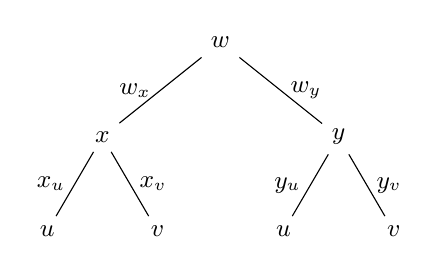
\begin{tikzpicture}[font=\small,level distance=1.2cm,
  level 1/.style={sibling distance=3cm},level 2/.style={sibling distance=1.4cm}]
  \node {$w$}
    child {node {$x$} child {node {$u$} edge from parent node[left] {$x_u$}} child {node {$v$} edge from parent node[right] {$x_v$}} edge from parent node[left] {$w_x$}}
    child {node {$y$} child {node {$u$} edge from parent node[left] {$y_u$}} child {node {$v$} edge from parent node[right] {$y_v$}} edge from parent node[right] {$w_y$}};
\end{tikzpicture}
\caption{Diagrama de árbol de $w=f(x,y)$ con $x=x(u,v)$, $y=y(u,v)$. Los dos caminos de $w$ a $u$ dan $w_u=w_xx_u+w_yy_u$.}
\label{fig:t4-arbol}
\end{figure}

\begin{ejemplo}\label{ej:t4-polares}
Sea $w=x^2+y^2$ con $x=r\cos\theta$, $y=r\sin\theta$. Por~\eqref{eq:t4-cadena2}, $w_r=2x\cos\theta+2y\sin\theta=2r$ y $w_\theta=2x(-r\sin\theta)+2y(r\cos\theta)=0$, como corresponde a $w=r^2$, que no depende de $\theta$.
\end{ejemplo}

\section{Gradiente y derivada direccional}

\begin{definicion}[Derivada direccional]\label{def:direccional}
Sea $\vu$ un vector \emph{unitario}. La \emph{derivada direccional} de $f$ en $\va$ según $\vu$ es
\[
D_{\vu}f(\va)=\lim_{t\to0}\frac{f(\va+t\vu)-f(\va)}{t},
\]
la tasa de cambio de $f$ por unidad de longitud recorrida en la dirección de $\vu$. Para $\vu=\vi$ y $\vu=\vj$ se obtienen $f_x$ y $f_y$.
\end{definicion}

\begin{teorema}[Cálculo de la derivada direccional]\label{teo:direccional}
Si $f$ es diferenciable en $\va$, entonces $D_{\vu}f(\va)=\nabla f(\va)\cdot\vu$ para todo vector unitario $\vu$.
\end{teorema}

\begin{proof}
Es la regla de la cadena (\cref{teo:cadena}) aplicada a la recta $\vr(t)=\va+t\vu$, cuya velocidad es $\vr\,'(0)=\vu$.
\end{proof}

\begin{corolario}[Dirección de máximo crecimiento]\label{cor:maximo-crecimiento}
Sea $\nabla f(\va)\neq\vcero$. Entre todas las direcciones unitarias, $D_{\vu}f(\va)$ alcanza su máximo, $\norm{\nabla f(\va)}$, para $\vu=\nabla f(\va)/\norm{\nabla f(\va)}$, su mínimo, $-\norm{\nabla f(\va)}$, en la dirección opuesta, y se anula en las direcciones perpendiculares al gradiente.
\end{corolario}

\begin{proof}
Por Cauchy--Schwarz (\cref{teo:cs}), $\abs{\nabla f\cdot\vu}\le\norm{\nabla f}\norm{\vu}=\norm{\nabla f}$, con igualdad si y solo si $\vu$ es múltiplo de $\nabla f$; los dos múltiplos unitarios dan $\pm\norm{\nabla f}$. Además $\nabla f\cdot\vu=\norm{\nabla f}\cos\theta$ es nulo exactamente cuando $\theta=\pi/2$.
\end{proof}

\begin{teorema}[El gradiente es normal a los conjuntos de nivel]\label{teo:gradiente-normal}
Sea $f$ diferenciable y $\vr(t)$ una curva derivable contenida en el conjunto de nivel $f=c$, con $\vr(t_0)=\va$. Entonces $\nabla f(\va)\cdot\vr\,'(t_0)=0$.
\end{teorema}

\begin{proof}
Como $f(\vr(t))=c$ para todo $t$, al derivar con la regla de la cadena se obtiene $0=\frac{d}{dt}f(\vr(t))=\nabla f(\vr(t))\cdot\vr\,'(t)$, y basta evaluar en $t_0$.
\end{proof}

En consecuencia, el \emph{plano tangente} a la superficie de nivel $F(x,y,z)=c$ en un punto $P_0$ con $\nabla F(P_0)\neq\vcero$ es el plano de normal $\nabla F(P_0)$: $\nabla F(P_0)\cdot(X-P_0)=0$. El plano tangente a una gráfica $z=f(x,y)$ es el caso particular $F(x,y,z)=f(x,y)-z$.

\begin{ejemplo}\label{ej:t4-direccional}
Para $f(x,y)=x^2y+y^3$ en $(1,2)$, $\nabla f=(4,13)$. En la dirección $\vu=(3,4)/5$, $D_{\vu}f=(12+52)/5=12{,}8$. La tasa máxima es $\norm{\nabla f}=\sqrt{185}\approx13{,}60$, en la dirección $(4,13)/\sqrt{185}$, y $f$ no varía, a primer orden, en las direcciones $\pm(13,-4)/\sqrt{185}$, tangentes a la curva de nivel $f=10$.
\end{ejemplo}

\begin{observacion}[Errores frecuentes]
\begin{enumerate}[label=(\alph*)]
\item La fórmula $D_{\vu}f=\nabla f\cdot\vu$ exige $\norm{\vu}=1$. Si la dirección viene dada por un vector $\vw$ cualquiera, hay que normalizarlo: $\vu=\vw/\norm{\vw}$.
\item El gradiente de $f(x,y)$ es un vector del plano $xy$ (del dominio), no de la superficie gráfica; es perpendicular a las curvas de nivel, no a la gráfica.
\item La existencia de derivadas parciales no garantiza la diferenciabilidad, ni siquiera la continuidad (\cref{eje:4-no-diferenciable}).
\item En la regla de la cadena hay que sumar las contribuciones de todos los caminos del árbol; omitir uno es el error más común.
\end{enumerate}
\end{observacion}

\begin{observacion}[Conexión con el curso]
El \cref{cor:maximo-crecimiento} es el fundamento del \emph{descenso de gradiente} $\mathbf w_{k+1}=\mathbf w_k-\eta\nabla L(\mathbf w_k)$ (módulo~7): cada paso se mueve en la dirección en que la pérdida $L$ decrece más deprisa. La regla de la cadena aplicada sistemáticamente a una composición de muchas funciones es la \emph{retropropagación} (módulo~10), y su forma matricial, con el jacobiano, se estudia en el módulo~4 (temas~1 y~2). El gradiente de la log-suma-exp es la softmax (\cref{eje:4-softmax}), lo que explica la sencillez del gradiente de la entropía cruzada (módulo~8).
\end{observacion}

\begin{lecturas}
\item MIT 18.02SC~\cite{mit1802}, unidad~2, parte~A, sesiones~26--27 (derivadas parciales, aproximación), y parte~B, sesiones~32--38 (diferenciales, regla de la cadena, gradiente, derivada direccional).
\item OpenStax \emph{Calculus}, vol.~3~\cite{openstax3}, §4.3 «Partial Derivatives», §4.4 «Tangent Planes and Linear Approximations», §4.5 «The Chain Rule» y §4.6 «Directional Derivatives and the Gradient».
\item Strang, \emph{Calculus}~\cite{strangcalc}, §13.2--13.5.
\item Apostol~\cite{apostol2}, cap.~8, para las demostraciones del teorema de Schwarz y de la condición suficiente de diferenciabilidad.
\end{lecturas}

\section*{Ejercicios del tema 4}
\addcontentsline{toc}{section}{Ejercicios del tema 4}

\begin{ejercicio}{1}{eje:4-conceptos}
Razone si son verdaderas o falsas: (a) $f_x(a,b)$ es la pendiente del corte de la gráfica con el plano $x=a$; (b) si $\nabla f(\va)=(3,4)$, la derivada de $f$ en la dirección de $\vw=(1,1)$ es $7$; (c) si $f$ tiene derivadas parciales en $\va$, es continua en $\va$; (d) si $\nabla f(\va)\neq\vcero$, la recta tangente en $\va$ a la curva de nivel que pasa por $\va$ es perpendicular a $\nabla f(\va)$.
\end{ejercicio}

\begin{ejercicio}{2}{eje:4-parciales}
Calcule las derivadas parciales primeras de: (a) $x^3y-3xy^2+2y^2$; (b) $x^2/y$; (c) $\sin(3x+2y)$; (d) $e^{xy}$; (e) $x\ln(2x+y)$; (f) $x^2z-2yz^3$.
\fuente{adaptado de MIT 18.02SC~\cite{mit1802}, problemas suplementarios, 2A-2.}
\end{ejercicio}

\begin{ejercicio}{2}{eje:4-schwarz}
Compruebe que $f_{xy}=f_{yx}$ para: (a) $x^my^n$, con $m,n$ enteros positivos; (b) $\cos(x^2+y)$; (c) $f(x)g(y)$, con $f,g$ derivables dos veces. (d) Compruebe también que $w=e^{ax}\sin(ay)$ satisface la ecuación de Laplace $w_{xx}+w_{yy}=0$.
\fuente{adaptado de MIT 18.02SC~\cite{mit1802}, problemas suplementarios, 2A-3 y 2A-5.}
\end{ejercicio}

\begin{ejercicio}{2}{eje:4-tangente}
Halle el plano tangente a la gráfica de: (a) $z=xy^2$ en $(1,1,1)$; (b) $z=e^{x}\cos y$ en $(0,0,1)$. Use (b) para aproximar $e^{0{,}1}\cos(0{,}1)$ y compare con el valor exacto.
\fuente{adaptado de MIT 18.02SC~\cite{mit1802}, problemas suplementarios, 2B-1 y 2B-5.}
\end{ejercicio}

\begin{ejercicio}{2}{eje:4-aproximacion}
(a) Los catetos de un triángulo rectángulo miden $3$ y $4$ y cada uno aumenta $0{,}01$. Estime con la aproximación lineal el cambio de la hipotenusa. (b) Una caja mide $5\times10\times20$~cm y cada medida tiene un error posible de $\pm0{,}1$~cm. Estime con diferenciales el error posible del volumen.
\fuente{adaptado de MIT 18.02SC~\cite{mit1802}, problemas suplementarios, 2B-3 y 2C-2.}
\end{ejercicio}

\begin{ejercicio}{2}{eje:4-gradiente}
Halle el gradiente en $P$ y la derivada direccional en $P$ en la dirección del vector $\va$: (a) $f=x^3+2y^3$, $P=(1,1)$, $\va=\vi-\vj$; (b) $w=xy/z$, $P=(2,-1,1)$, $\va=\vi+2\vj-2\vk$.
\fuente{adaptado de MIT 18.02SC~\cite{mit1802}, problemas suplementarios, 2D-1.}
\end{ejercicio}

\begin{ejercicio}{2}{eje:4-max-direccional}
Para $w=\ln(4x-3y)$ en $(1,1)$, halle: (a) el máximo y el mínimo de la derivada direccional y las direcciones en que se alcanzan; (b) las direcciones en que la derivada direccional es nula.
\fuente{adaptado de MIT 18.02SC~\cite{mit1802}, problemas suplementarios, 2D-2.}
\end{ejercicio}

\begin{ejercicio}{2}{eje:4-tangente-nivel}
Halle el plano tangente a la superficie, vista como superficie de nivel, en el punto indicado: (a) $xy^2z^3=12$ en $(3,2,1)$; (b) el elipsoide $x^2+4y^2+9z^2=14$ en $(1,1,1)$.
\fuente{adaptado de MIT 18.02SC~\cite{mit1802}, problemas suplementarios, 2D-3.}
\end{ejercicio}

\begin{ejercicio}{2}{eje:4-cadena-t}
Calcule $dw/dt$ de dos maneras, con la regla de la cadena y sustituyendo antes de derivar: (a) $w=xyz$ con $x=t$, $y=t^2$, $z=t^3$; (b) $w=x^2-y^2$ con $x=\cos t$, $y=\sin t$.
\fuente{adaptado de MIT 18.02SC~\cite{mit1802}, problemas suplementarios, 2E-1.}
\end{ejercicio}

\begin{ejercicio}{2}{eje:4-cadena-uv}
Sea $w=f(x,y)$ con $\nabla f(0,1)=(2,3)$, y sean $x=u^2-v^2$, $y=uv$. Calcule $\partial w/\partial u$ y $\partial w/\partial v$ en $(u,v)=(1,1)$.
\fuente{adaptado de MIT 18.02SC~\cite{mit1802}, problemas suplementarios, 2E-4.}
\end{ejercicio}

\begin{ejercicio}{2}{eje:4-softmax}
Sea $f(x,y)=\ln(e^x+e^y)$. (a) Demuestre que $\nabla f=(\sigma_1,\sigma_2)$ con $\sigma_1=\dfrac{e^x}{e^x+e^y}$, $\sigma_2=\dfrac{e^y}{e^x+e^y}$, y que $\sigma_1,\sigma_2\in(0,1)$ con $\sigma_1+\sigma_2=1$. (b) Calcule la derivada direccional en la dirección $(1,1)/\sqrt2$ y explique el resultado a partir de $f(x+t,y+t)$. (c) Aproxime linealmente $f(1{,}1;\,-0{,}1)$ desde $(1,0)$ y compare con el valor exacto.
\end{ejercicio}

\begin{ejercicio}{3}{eje:4-polares}
Sea $w=f(x,y)$ diferenciable, con $x=r\cos\theta$, $y=r\sin\theta$ y $r>0$. Demuestre que
\[
w_x^2+w_y^2=w_r^2+\frac{1}{r^2}w_\theta^2 .
\]
\fuente{adaptado de MIT 18.02SC~\cite{mit1802}, problemas suplementarios, 2E-5.}
\end{ejercicio}

\begin{ejercicio}{3}{eje:4-euler}
(a) Sea $f$ derivable en una variable y $w=f(y/x)$ para $x\neq0$. Demuestre que $xw_x+yw_y=0$. (b) Una función $g(x,y)$ es \emph{homogénea de grado $k$} si $g(tx,ty)=t^kg(x,y)$ para todo $t>0$. Demuestre que, si es diferenciable, cumple la \emph{identidad de Euler} $xg_x+yg_y=k\,g$. (c) Compruébela para $g=x^2y+y^3$.
\fuente{adaptado de MIT 18.02SC~\cite{mit1802}, problemas suplementarios, 2E-8.}
\end{ejercicio}

\begin{ejercicio}{3}{eje:4-material}
Sea $f(x,y,z,t)$ diferenciable y $\vr(t)=(x(t),y(t),z(t))$ la trayectoria de una partícula, con velocidad $\vv=\vr\,'(t)$. Sea $\nabla f$ el gradiente respecto de las variables espaciales. Demuestre que la \emph{derivada material} $\frac{Df}{Dt}=\frac{d}{dt}f(\vr(t),t)$ vale
\[
\frac{Df}{Dt}=\pd ft+\vv\cdot\nabla f .
\]
\fuente{adaptado de MIT 18.02SC~\cite{mit1802}, \emph{problem set}~5, parte~II, problema~2.}
\end{ejercicio}

\begin{ejercicio}{3}{eje:4-no-diferenciable}
Sea $f(x,y)=\dfrac{xy}{x^2+y^2}$ si $(x,y)\neq(0,0)$ y $f(0,0)=0$. (a) Demuestre que $f_x(0,0)$ y $f_y(0,0)$ existen y valen~$0$. (b) Demuestre que $f$ no es diferenciable en el origen. (c) Calcule, para $\vu=(1,1)/\sqrt2$, el cociente $\bigl(f(t\vu)-f(\vcero)\bigr)/t$ y explique por qué la derivada direccional $D_{\vu}f(\vcero)$ no existe, aunque $\nabla f(\vcero)\cdot\vu=0$.
\end{ejercicio}

% =====================================================================
\chapter{Extremos libres y condicionados}
\label{tema:5}
% =====================================================================

Entrenar un modelo es minimizar una función de muchas variables, y estimar probabilidades por máxima verosimilitud es maximizar una función con la restricción de que las probabilidades sumen uno. Este tema estudia ambos problemas en dimensión dos y tres: los extremos libres, que se localizan donde se anula el gradiente y se clasifican con la matriz hessiana, y los extremos condicionados, que se resuelven con multiplicadores de Lagrange. La presentación sigue las sesiones~28--31 y~39--40 de 18.02SC~\cite{mit1802}, las §4.7--4.8 de OpenStax~\cite{openstax3}, las §9.9--9.12 y~9.14 de Apostol~\cite{apostol2}, el texto de Marsden y Tromba~\cite{marsden} y las §13.6--13.7 de Strang~\cite{strangcalc}.

\section{Extremos locales y puntos críticos}

\begin{definicion}[Extremos]\label{def:extremos}
Sea $f:D\subseteq\R^n\to\R$ y $\va\in D$. Se dice que $f$ tiene en $\va$ un \emph{máximo local} si existe $\delta>0$ tal que $f(\vx)\le f(\va)$ para todo $\vx\in D$ con $\norm{\vx-\va}<\delta$; un \emph{mínimo local}, con $\ge$. Si la desigualdad vale para todo $\vx\in D$, el extremo es \emph{absoluto} (o global). Un punto $\va$ interior al dominio es \emph{crítico} si $\nabla f(\va)=\vcero$ o si alguna derivada parcial no existe en $\va$.
\end{definicion}

\begin{teorema}[Condición necesaria de Fermat]\label{teo:fermat}
Si $f$ tiene un extremo local en un punto interior $\va$ y sus derivadas parciales existen en $\va$, entonces $\nabla f(\va)=\vcero$.
\end{teorema}

\begin{proof}
Sea $i\in\{1,\dots,n\}$ y $\varphi(t)=f(\va+t\mathbf e_i)$, definida para $t$ pequeño porque $\va$ es interior. La función de una variable $\varphi$ tiene un extremo local en $t=0$ y es derivable allí con $\varphi'(0)=f_{x_i}(\va)$. Por el teorema de Fermat de una variable, $\varphi'(0)=0$.
\end{proof}

El recíproco es falso: $f(x,y)=x^2-y^2$ tiene $\nabla f(0,0)=\vcero$ y no tiene extremo en el origen, pues crece a lo largo del eje $x$ y decrece a lo largo del eje $y$. Un punto crítico que no es extremo local se llama \emph{punto de silla}.

\section{Clasificación: el criterio del hessiano}

\begin{definicion}[Matriz hessiana]\label{def:hessiana}
Si $f(x,y)$ tiene derivadas segundas, su \emph{matriz hessiana} y su \emph{discriminante} en $\va$ son
\[
H_f(\va)=\begin{pmatrix}f_{xx}&f_{xy}\\f_{yx}&f_{yy}\end{pmatrix}(\va),\qquad
\Delta(\va)=\det H_f(\va)=f_{xx}f_{yy}-f_{xy}^2 ,
\]
donde se ha usado el teorema de Schwarz para escribir $f_{xy}=f_{yx}$.
\end{definicion}

La idea del criterio es la fórmula de Taylor de segundo orden: si $f$ tiene derivadas segundas continuas y $\nabla f(\va)=\vcero$, entonces, con $\mathbf h=(h,k)$,
\begin{equation}\label{eq:t5-taylor}
f(\va+\mathbf h)=f(\va)+\tfrac12\,Q(\mathbf h)+\varepsilon(\mathbf h)\norm{\mathbf h}^2,\qquad Q(h,k)=Ah^2+2Bhk+Ck^2,
\end{equation}
con $A=f_{xx}(\va)$, $B=f_{xy}(\va)$, $C=f_{yy}(\va)$ y $\varepsilon(\mathbf h)\to0$. La demostración de~\eqref{eq:t5-taylor} aplica la fórmula de Taylor de una variable a $t\mapsto f(\va+t\mathbf h)$ (Apostol~\cite[§9.9--9.12]{apostol2}; módulo~4, tema~4). Cerca de un punto crítico, por tanto, el signo de $f(\va+\mathbf h)-f(\va)$ lo decide la \emph{forma cuadrática} $Q$.

\begin{lema}[Signo de una forma cuadrática]\label{lem:forma}
Sea $Q(h,k)=Ah^2+2Bhk+Ck^2$ y $\Delta=AC-B^2$.
\begin{enumerate}
  \item Si $\Delta>0$ y $A>0$, entonces $Q(h,k)>0$ para todo $(h,k)\neq(0,0)$.
  \item Si $\Delta>0$ y $A<0$, entonces $Q(h,k)<0$ para todo $(h,k)\neq(0,0)$.
  \item Si $\Delta<0$, $Q$ toma valores positivos y negativos.
\end{enumerate}
\end{lema}

\begin{proof}
Si $A\neq0$, completando el cuadrado,
\[
Q(h,k)=A\Bigl(h+\frac BAk\Bigr)^2+\frac{AC-B^2}{A}k^2=\frac1A\Bigl[(Ah+Bk)^2+\Delta k^2\Bigr].
\]
(i) Si $\Delta>0$ y $A>0$, el corchete es suma de dos términos no negativos que solo se anulan a la vez si $k=0$ y $Ah+Bk=Ah=0$, es decir, si $(h,k)=(0,0)$. (ii) Es (i) aplicado a $-Q$. (iii) Si $\Delta<0$ y $A\neq0$: con $k=0$, $h=1$, $Q=A$; con $k=1$, $h=-B/A$, $Q=\Delta/A$, de signo contrario a $A$. Si $A=0$, entonces $\Delta=-B^2<0$ obliga a $B\neq0$, y $Q(h,1)=2Bh+C$ toma ambos signos al variar $h$.
\end{proof}

\begin{teorema}[Criterio del hessiano]\label{teo:hessiano}
Sea $f$ con derivadas segundas continuas cerca de un punto crítico $\va$ con $\nabla f(\va)=\vcero$, y sea $\Delta=\Delta(\va)$.
\begin{enumerate}
  \item Si $\Delta>0$ y $f_{xx}(\va)>0$, $f$ tiene un mínimo local en $\va$.
  \item Si $\Delta>0$ y $f_{xx}(\va)<0$, $f$ tiene un máximo local en $\va$.
  \item Si $\Delta<0$, $\va$ es un punto de silla.
  \item Si $\Delta=0$, el criterio no decide.
\end{enumerate}
\end{teorema}

\begin{proof}[Idea de la demostración]
(i) Por el \cref{lem:forma}, $Q>0$ en la circunferencia unidad, que es cerrada y acotada; por el teorema de Weierstrass (\cref{teo:weierstrass}) alcanza allí un mínimo $m>0$, y por homogeneidad $Q(\mathbf h)\ge m\norm{\mathbf h}^2$. En~\eqref{eq:t5-taylor}, si $\norm{\mathbf h}$ es tan pequeño que $\abs{\varepsilon(\mathbf h)}<m/4$, se obtiene $f(\va+\mathbf h)-f(\va)\ge\frac m4\norm{\mathbf h}^2>0$. (ii) se reduce a (i) con $-f$. (iii) Si $Q(\mathbf h_1)>0>Q(\mathbf h_2)$, a lo largo de las rectas $t\mathbf h_1$ y $t\mathbf h_2$ la función crece y decrece respectivamente para $t$ pequeño, por el mismo argumento. (iv) Lo muestran los ejemplos del \cref{eje:5-degenerado}.
\end{proof}

\begin{ejemplo}\label{ej:t5-hessiano}
(a) $f(x,y)=x^2+xy+y^2-3x$: $f_x=2x+y-3$ y $f_y=x+2y$ se anulan en $(2,-1)$. La hessiana es constante, $\begin{pmatrix}2&1\\1&2\end{pmatrix}$, con $\Delta=3>0$ y $f_{xx}=2>0$: mínimo local, de valor $f(2,-1)=-3$.

(b) $g(x,y)=x^3-3x+y^2$: $g_x=3x^2-3$ y $g_y=2y$ se anulan en $(\pm1,0)$. Como $H_g=\begin{pmatrix}6x&0\\0&2\end{pmatrix}$, en $(1,0)$ es $\Delta=12>0$ con $g_{xx}=6>0$ (mínimo local, $g=-2$), y en $(-1,0)$ es $\Delta=-12<0$ (punto de silla).
\end{ejemplo}

\section{Extremos absolutos en regiones cerradas y acotadas}

\begin{teorema}[Weierstrass]\label{teo:weierstrass}
Una función continua sobre un conjunto cerrado y acotado de $\R^n$ alcanza en él un máximo y un mínimo absolutos.
\end{teorema}

La demostración usa la completitud de los números reales y se omite; para una variable es el teorema de los valores extremos del cálculo elemental. En la práctica, para hallar los extremos absolutos de $f$ en una región $R$ cerrada y acotada: (1) se hallan los puntos críticos interiores; (2) se estudia $f$ sobre la frontera, que suele reducirse a funciones de una variable o a un problema con multiplicadores de Lagrange; (3) se comparan todos los valores obtenidos.

\begin{ejemplo}\label{ej:t5-absolutos}
Extremos de $f(x,y)=x^2+y^2-2x$ en el disco $x^2+y^2\le4$. Interior: $\nabla f=(2x-2,2y)=\vcero$ en $(1,0)$, con $f(1,0)=-1$. Frontera: si $x^2+y^2=4$, $f=4-2x$ con $x\in[-2,2]$, que varía entre $0$ (en $(2,0)$) y $8$ (en $(-2,0)$). Comparando: el máximo absoluto es $8$, en $(-2,0)$, y el mínimo absoluto es $-1$, en $(1,0)$.
\end{ejemplo}

\section{Multiplicadores de Lagrange}

Se busca el máximo o el mínimo de $f(x,y)$ cuando $(x,y)$ está obligado a moverse sobre la curva $g(x,y)=c$. En un extremo, la curva de nivel de $f$ que pasa por el punto no puede cruzar la restricción, porque entonces se podría seguir avanzando sobre $g=c$ hacia valores mayores y menores de $f$: ambas curvas deben ser \emph{tangentes}, y sus gradientes, paralelos (\cref{fig:t5-lagrange}).

\begin{figure}[ht]
\centering
\begin{tikzpicture}[scale=1.15,>={Stealth[length=2mm]},font=\small]
  \draw[->] (-1.9,0) -- (2.4,0) node[right] {$x$};
  \draw[->] (0,-1.9) -- (0,2.4) node[above] {$y$};
  \draw[thick] (0,0) circle ({sqrt(2)});
  \foreach \c in {0,1,2,3} \draw[gray,dashed] ({\c-2.2},2.2) -- (2.2,{\c-2.2});
  \fill (1,1) circle (1.6pt);
  \draw[->,thick] (1,1) -- (1.55,1.55) node[above right] {$\nabla f\parallel\nabla g$};
  \node at (-1.25,-1.45) {$g=2$};
  \node[gray] at (2.15,-0.45) {$f=c$};
\end{tikzpicture}
\caption{Máximo de $f(x,y)=x+y$ sobre la circunferencia $g(x,y)=x^2+y^2=2$. Las rectas de nivel de $f$ (discontinuas) cortan a la circunferencia salvo la de nivel $2$, que es tangente en $(1,1)$; allí $\nabla f=(1,1)$ y $\nabla g=(2,2)$ son paralelos.}
\label{fig:t5-lagrange}
\end{figure}

\begin{teorema}[Multiplicadores de Lagrange]\label{teo:lagrange}
Sean $f$ y $g$ funciones de $(x,y)$ con derivadas parciales continuas, y sea $\va$ un punto de la curva $g=c$ con $\nabla g(\va)\neq\vcero$. Si $f$, restringida a la curva, tiene un extremo local en $\va$, existe $\lambda\in\R$ (el \emph{multiplicador}) tal que
\[
\nabla f(\va)=\lambda\nabla g(\va).
\]
El mismo enunciado vale para $f$ y $g$ de tres variables y la superficie $g=c$.
\end{teorema}

\begin{proof}
Como $\nabla g(\va)\neq\vcero$, el teorema de la función implícita~\cite[§9.6--9.7]{apostol2} asegura que, cerca de $\va$, la curva $g=c$ es la trayectoria de una curva derivable $\vr(t)$ con $\vr(0)=\va$ y $\vr\,'(0)\neq\vcero$. La función de una variable $t\mapsto f(\vr(t))$ tiene un extremo local en $t=0$, luego, por la regla de la cadena, $0=\nabla f(\va)\cdot\vr\,'(0)$. Además $\nabla g(\va)\cdot\vr\,'(0)=0$ por el \cref{teo:gradiente-normal}. En el plano, los vectores perpendiculares al vector no nulo $\vr\,'(0)$ forman una recta, de modo que $\nabla f(\va)$ y $\nabla g(\va)$ son proporcionales; como $\nabla g(\va)\neq\vcero$, $\nabla f(\va)=\lambda\nabla g(\va)$. En $\R^3$ el argumento se aplica a todas las curvas de la superficie que pasan por $\va$: $\nabla f(\va)$ es perpendicular a su plano tangente y, por tanto, paralelo a la normal $\nabla g(\va)$.
\end{proof}

El método consiste en resolver el sistema formado por $\nabla f=\lambda\nabla g$ y $g=c$ (tres ecuaciones con incógnitas $x,y,\lambda$ en el plano; cuatro en el espacio). Sus soluciones son los \emph{candidatos}; si la restricción es cerrada y acotada, el teorema de Weierstrass garantiza que el mayor valor de $f$ entre ellos es el máximo y el menor, el mínimo.

\begin{ejemplo}\label{ej:t5-lagrange-circulo}
Extremos de $f=x+y$ sobre $x^2+y^2=2$. Las ecuaciones $1=2\lambda x$, $1=2\lambda y$ dan $x=y=1/(2\lambda)$, y la restricción, $2x^2=2$, luego $x=\pm1$. Candidatos: $(1,1)$, con $f=2$, y $(-1,-1)$, con $f=-2$. La circunferencia es cerrada y acotada: el máximo es $2$ y el mínimo $-2$.
\end{ejemplo}

\begin{ejemplo}\label{ej:t5-lagrange-plano}
El punto del plano $x+2y+2z=9$ más cercano al origen minimiza $f=x^2+y^2+z^2$ con $g=x+2y+2z=9$. Las ecuaciones $2x=\lambda$, $2y=2\lambda$, $2z=2\lambda$ dan $(x,y,z)=(\lambda/2,\lambda,\lambda)$; sustituyendo, $\tfrac{9}{2}\lambda=9$, $\lambda=2$ y el punto es $(1,2,2)$, a distancia~$3$ del origen, de acuerdo con la fórmula $\abs d/\norm{\vn}=9/3$ del \cref{eje:2-distancia}. Aquí la restricción no es acotada, pero $f$ crece sin límite al alejarse, de modo que el único candidato es el mínimo.
\end{ejemplo}

\begin{observacion}[Errores frecuentes]
\begin{enumerate}[label=(\alph*)]
\item $\nabla f=\vcero$ no implica extremo (puntos de silla); y con $\Delta=0$ no se puede concluir nada sin un análisis adicional.
\item El criterio del hessiano sirve para puntos críticos interiores; en la frontera de una región los extremos se buscan aparte.
\item Lagrange proporciona \emph{candidatos}, no extremos: hay que comparar sus valores y justificar la existencia del máximo o del mínimo.
\item Al resolver $\nabla f=\lambda\nabla g$ no se debe dividir por una variable que pueda anularse; se pierden soluciones (\cref{eje:5-hiperbola}).
\end{enumerate}
\end{observacion}

\begin{observacion}[Conexión con el curso]
El estimador de máxima verosimilitud de un modelo de bigramas (módulo~1, tema~3) maximiza $\sum_i n_i\ln p_i$ con la restricción $\sum_ip_i=1$; con un multiplicador de Lagrange resulta la frecuencia relativa $p_i=n_i/N$ (\cref{eje:5-mle}). El mismo método demuestra que la distribución de máxima entropía sobre $K$ valores es la uniforme (módulo~6). La hessiana y su relación con la convexidad y con la velocidad del descenso de gradiente se desarrollan en los módulos~4 (tema~4) y~7, y la recta de mínimos cuadrados (\cref{eje:5-minimos-cuadrados}) es el punto de partida de la regresión lineal del módulo~8.
\end{observacion}

\begin{lecturas}
\item MIT 18.02SC~\cite{mit1802}, unidad~2, parte~A, sesiones~28--31 (optimización, mínimos cuadrados, criterio de la derivada segunda), y parte~C, sesiones~39--40 (multiplicadores de Lagrange y su demostración).
\item OpenStax \emph{Calculus}, vol.~3~\cite{openstax3}, §4.7 «Maxima/Minima Problems» y §4.8 «Lagrange Multipliers».
\item Apostol~\cite{apostol2}, §9.9--9.12 (hessiana, criterio de la derivada segunda, fórmula de Taylor) y §9.14 (extremos condicionados y multiplicadores de Lagrange).
\item Strang, \emph{Calculus}~\cite{strangcalc}, §13.6 «Maxima, Minima, and Saddle Points» y §13.7 «Constraints and Lagrange Multipliers».
\end{lecturas}

\section*{Ejercicios del tema 5}
\addcontentsline{toc}{section}{Ejercicios del tema 5}

\begin{ejercicio}{1}{eje:5-conceptos}
Razone si son verdaderas o falsas: (a) si $\nabla f(\va)=\vcero$, entonces $f$ tiene un extremo local en $\va$; (b) si en un punto crítico $\Delta=0$, el punto es de silla; (c) toda solución del sistema de Lagrange es un máximo o un mínimo condicionado; (d) una función continua en el disco abierto $x^2+y^2<1$ alcanza siempre su máximo.
\end{ejercicio}

\begin{ejercicio}{2}{eje:5-clasificar-1}
Halle y clasifique los puntos críticos de: (a) $x^2-xy-2y^2-3x-3y+1$; (b) $3x^2+xy+y^2-x-2y+4$.
\fuente{adaptado de MIT 18.02SC~\cite{mit1802}, problemas suplementarios, 2H-1.}
\end{ejercicio}

\begin{ejercicio}{2}{eje:5-clasificar-2}
Halle y clasifique los puntos críticos de $f(x,y)=x^3-3xy+y^3$.
\fuente{adaptado de MIT 18.02SC~\cite{mit1802}, problemas suplementarios, 2H-1.}
\end{ejercicio}

\begin{ejercicio}{2}{eje:5-clasificar-3}
Halle y clasifique los puntos críticos de $f(x,y)=2x^4+y^2-xy+1$.
\fuente{adaptado de MIT 18.02SC~\cite{mit1802}, problemas suplementarios, 2H-1.}
\end{ejercicio}

\begin{ejercicio}{2}{eje:5-openstax}
Halle y clasifique los puntos críticos de: (a) $f(x,y)=x^3+2xy-2x-4y$; (b) $g(x,y)=4x^2+9y^2+8x-36y+24$. En (b), confirme el resultado completando cuadrados.
\fuente{adaptado de OpenStax \emph{Calculus}, vol.~3~\cite{openstax3}, §4.7, punto de control~4.34 y ejemplo~4.39.}
\end{ejercicio}

\begin{ejercicio}{2}{eje:5-absolutos}
Halle el máximo y el mínimo absolutos de $f(x,y)=xy-x-y+2$ en el cuadrado $0\le x\le2$, $0\le y\le2$. (Indicación: $f=(x-1)(y-1)+1$.)
\fuente{adaptado de MIT 18.02SC~\cite{mit1802}, problemas suplementarios, 2H-4.}
\end{ejercicio}

\begin{ejercicio}{2}{eje:5-disco}
Halle el máximo y el mínimo de $f(x,y)=x+\sqrt3\,y+2$ en el disco $x^2+y^2\le1$.
\fuente{adaptado de MIT 18.02SC~\cite{mit1802}, problemas suplementarios, 2H-5.}
\end{ejercicio}

\begin{ejercicio}{2}{eje:5-caja}
Una caja rectangular del primer octante tiene un vértice en el origen, caras sobre los planos coordenados y el vértice opuesto $P=(x,y,z)$ sobre el plano $x+2y+3z=18$. Halle con multiplicadores de Lagrange el $P$ que maximiza el volumen y justifique que es un máximo.
\fuente{adaptado de MIT 18.02SC~\cite{mit1802}, problemas suplementarios, 2I-1.}
\end{ejercicio}

\begin{ejercicio}{2}{eje:5-hiperbola}
Halle los extremos de $f(x,y)=x^2-y^2$ sobre la circunferencia $x^2+y^2=3$ con multiplicadores de Lagrange. Indique, para cada solución, el valor de $\lambda$ y si $\nabla f$ y $\nabla g$ tienen el mismo sentido o sentidos opuestos.
\fuente{adaptado de MIT 18.02SC~\cite{mit1802}, \emph{problem set}~6, parte~II, problema~1.}
\end{ejercicio}

\begin{ejercicio}{2}{eje:5-resistencias}
Una corriente $I>0$ se reparte entre dos resistencias en paralelo, $R_1$ y $R_2$, en corrientes $I_1+I_2=I$. La potencia disipada es $I_1^2R_1+I_2^2R_2$. Halle el reparto que la minimiza y compruebe que es el de las leyes de Kirchhoff ($I_1R_1=I_2R_2$).
\fuente{adaptado de MIT 18.02SC~\cite{mit1802}, \emph{problem set}~6, parte~II, problema~2.}
\end{ejercicio}

\begin{ejercicio}{2}{eje:5-minimos-cuadrados}
Halle la recta $y=ax+b$ que minimiza $D(a,b)=\sum_{i=1}^{3}\bigl(y_i-(ax_i+b)\bigr)^2$ para los puntos $(1,1)$, $(2,3)$, $(3,2)$, y compruebe con el criterio del hessiano que el punto crítico es un mínimo.
\fuente{adaptado de MIT 18.02SC~\cite{mit1802}, problemas suplementarios, 2G-1.}
\end{ejercicio}

\begin{ejercicio}{3}{eje:5-degenerado}
Demuestre que $f_1=x^4+y^4$, $f_2=-x^4-y^4$ y $f_3=x^4-y^4$ tienen todas un punto crítico en el origen con $\Delta=0$, y que en él $f_1$ tiene un mínimo, $f_2$ un máximo y $f_3$ un punto de silla. ¿Qué concluye sobre el caso~(iv) del \cref{teo:hessiano}?
\end{ejercicio}

\begin{ejercicio}{3}{eje:5-mle}
Sean $n_1,\dots,n_K>0$ los recuentos de $K$ símbolos en un corpus y $N=\sum_in_i$. Se quiere maximizar la log-verosimilitud $\ell(p_1,\dots,p_K)=\sum_{i=1}^{K}n_i\ln p_i$ con $p_i>0$ y $\sum_ip_i=1$. (a) Demuestre con un multiplicador de Lagrange que el único candidato es $\hat p_i=n_i/N$. (b) Demuestre que es el máximo absoluto usando la desigualdad $\ln t\le t-1$ para $t>0$.
\end{ejercicio}

\begin{ejercicio}{3}{eje:5-media-geometrica}
(a) Demuestre que el máximo de $xyz$ sobre $x+y+z=S$, $x,y,z\ge0$ ($S>0$ fijo) existe, se alcanza en el interior y vale $(S/3)^3$. (b) Deduzca la desigualdad entre las medias aritmética y geométrica: $\sqrt[3]{abc}\le\frac{a+b+c}{3}$ para $a,b,c\ge0$.
\end{ejercicio}

\begin{ejercicio}{3}{eje:5-cs-lagrange}
Sea $\va\in\R^3$ no nulo. (a) Halle con multiplicadores de Lagrange el máximo y el mínimo de $f(\vx)=\va\cdot\vx$ sobre la esfera unidad $\norm{\vx}=1$. (b) Deduzca de nuevo la desigualdad de Cauchy--Schwarz. (c) Interprete el resultado a la luz del \cref{cor:maximo-crecimiento}.
\end{ejercicio}

% =====================================================================
\chapter{Integrales dobles y la integral gaussiana}
\label{tema:6}
% =====================================================================

La integral de una variable suma los valores de una función a lo largo de un intervalo; la integral doble los suma sobre una región del plano y mide, por ejemplo, el volumen bajo una superficie. Su cálculo se reduce a dos integrales de una variable sucesivas (teorema de Fubini), y en regiones circulares conviene usar coordenadas polares. La aplicación más importante para el curso es el cálculo de la integral gaussiana $\int_{-\infty}^{\infty}e^{-x^2}dx=\sqrt\pi$, que no puede obtenerse con primitivas elementales y sí con un rodeo por el plano. La presentación sigue las sesiones~47--54 de 18.02SC~\cite{mit1802}, las §5.1--5.3 de OpenStax~\cite{openstax3}, las §11.1--11.14 de Apostol~\cite{apostol2} y las §14.1--14.2 de Strang~\cite{strangcalc}.

\section{Integral doble sobre un rectángulo}

Sea $R=[a,b]\times[c,d]$ y $f$ acotada en $R$. Se divide $[a,b]$ en $m$ subintervalos de longitud $\Delta x$ y $[c,d]$ en $n$ de longitud $\Delta y$, lo que divide $R$ en $mn$ rectángulos $R_{ij}$ de área $\Delta A=\Delta x\,\Delta y$, y se elige un punto $(x_{ij}^*,y_{ij}^*)$ en cada uno.

\begin{definicion}[Integral doble]\label{def:integral-doble}
La \emph{integral doble} de $f$ sobre $R$ es
\[
\iint_R f(x,y)\dA=\lim_{m,n\to\infty}\sum_{i=1}^{m}\sum_{j=1}^{n}f(x_{ij}^*,y_{ij}^*)\,\Delta A ,
\]
si el límite existe y no depende de la elección de los puntos; se dice entonces que $f$ es \emph{integrable} en $R$. Toda función continua en $R$ es integrable.
\end{definicion}

Si $f\ge0$, cada sumando es el volumen de un prisma de base $R_{ij}$ y altura $f(x_{ij}^*,y_{ij}^*)$, y la integral es el \emph{volumen} del sólido comprendido entre $R$ y la gráfica de $f$. Si $f=1$, la integral es el área de $R$.

\begin{proposicion}[Propiedades]\label{prop:propiedades-integral}
Para $f,g$ integrables en $R$ y $\alpha,\beta\in\R$:
\begin{enumerate}
  \item linealidad: $\iint_R(\alpha f+\beta g)\dA=\alpha\iint_Rf\dA+\beta\iint_Rg\dA$;
  \item monotonía: si $f\le g$ en $R$, entonces $\iint_Rf\dA\le\iint_Rg\dA$;
  \item aditividad: si $R$ se divide en dos regiones $R_1$, $R_2$ que solo comparten frontera, $\iint_R f=\iint_{R_1}f+\iint_{R_2}f$.
\end{enumerate}
\end{proposicion}

Las tres propiedades se heredan de las sumas de Riemann al pasar al límite: por ejemplo, si $f\le g$, cada suma de $f$ es menor o igual que la correspondiente de $g$. El cálculo efectivo se apoya en el teorema siguiente, cuya demostración puede verse en Apostol~\cite[§11.10--11.11]{apostol2}.

\begin{teorema}[Fubini, para rectángulos]\label{teo:fubini}
Si $f$ es continua en $R=[a,b]\times[c,d]$, entonces
\[
\iint_R f\dA=\int_a^b\left(\int_c^d f(x,y)\,dy\right)dx=\int_c^d\left(\int_a^b f(x,y)\,dx\right)dy .
\]
\end{teorema}

En la integral interior $\int_c^df(x,y)\,dy$, la variable $x$ se trata como constante. Geométricamente, es el área de la sección del sólido por el plano vertical de abscisa $x$, y el volumen se obtiene sumando secciones.

\begin{corolario}[Integrandos separables]\label{cor:separable}
Si $f(x,y)=g(x)h(y)$ con $g$ y $h$ continuas, entonces $\iint_{[a,b]\times[c,d]}g(x)h(y)\dA=\left(\int_a^bg\right)\left(\int_c^dh\right)$.
\end{corolario}

\begin{proof}
Por Fubini, la integral es $\int_a^b\bigl(\int_c^dg(x)h(y)\,dy\bigr)dx$. En la integral interior $g(x)$ es constante: $\int_c^dg(x)h(y)\,dy=g(x)\int_c^dh$. Sacando la constante $\int_c^dh$ de la integral exterior se obtiene el resultado.
\end{proof}

\begin{ejemplo}\label{ej:t6-rectangulo}
$\iint_{[0,2]\times[0,3]}xy^2\dA=\int_0^2x\,dx\cdot\int_0^3y^2\,dy=2\cdot9=18$. Con Fubini sin separar: $\int_0^2\bigl[\tfrac{xy^3}{3}\bigr]_{y=0}^{y=3}dx=\int_0^29x\,dx=18$.
\end{ejemplo}

\section{Regiones generales y cambio del orden de integración}

\begin{definicion}[Regiones elementales]\label{def:regiones}
Una región es \emph{de tipo~I} si es de la forma $\{a\le x\le b,\ g_1(x)\le y\le g_2(x)\}$, y \emph{de tipo~II} si es $\{c\le y\le d,\ h_1(y)\le x\le h_2(y)\}$, con $g_i$, $h_i$ continuas.
\end{definicion}

Para $f$ continua, el teorema de Fubini se extiende a estas regiones~\cite[§11.12--11.14]{apostol2}:
\begin{align*}
\iint_Df\dA&=\int_a^b\int_{g_1(x)}^{g_2(x)}f(x,y)\,dy\,dx&&\text{(tipo I)},\\
\iint_Df\dA&=\int_c^d\int_{h_1(y)}^{h_2(y)}f(x,y)\,dx\,dy&&\text{(tipo II)}.
\end{align*}
Los límites de la integral interior pueden depender de la variable exterior; los de la exterior han de ser constantes. El método práctico es: dibujar la región, fijar la variable exterior y leer, sobre un segmento vertical (tipo~I) u horizontal (tipo~II), dónde entra y dónde sale de la región.

\begin{ejemplo}\label{ej:t6-region}
Sea $D$ la región entre $y=x^2$ e $y=x$ para $0\le x\le1$ (las curvas se cortan en $x=0$ y $x=1$, y $x^2\le x$ en medio). Entonces
\[
\iint_D(x+y)\dA=\int_0^1\int_{x^2}^{x}(x+y)\,dy\,dx=\int_0^1\Bigl(\tfrac32x^2-x^3-\tfrac12x^4\Bigr)dx=\tfrac12-\tfrac14-\tfrac1{10}=\tfrac{3}{20}.
\]
\end{ejemplo}

Cuando la integral interior no tiene primitiva elemental, puede bastar con cambiar el orden. Hay que describir la \emph{misma} región del otro modo.

\begin{ejemplo}\label{ej:t6-orden}
La integral $\int_0^1\int_x^1\sin(y^2)\,dy\,dx$ no puede calcularse en ese orden. La región es el triángulo $\{0\le x\le1,\ x\le y\le1\}$, que como región de tipo~II es $\{0\le y\le1,\ 0\le x\le y\}$. Por tanto,
\[
\int_0^1\int_0^y\sin(y^2)\,dx\,dy=\int_0^1y\sin(y^2)\,dy=\Bigl[-\tfrac12\cos(y^2)\Bigr]_0^1=\frac{1-\cos1}{2}\approx0{,}2298 .
\]
\end{ejemplo}

\section{Coordenadas polares}

En polares, $x=r\cos\theta$, $y=r\sin\theta$, con $r\ge0$. Las regiones naturales son los \emph{rectángulos polares} $\{r_1\le r\le r_2,\ \theta_1\le\theta\le\theta_2\}$, sectores de corona circular. Su área es la diferencia de dos sectores circulares:
\[
\tfrac12r_2^2\Delta\theta-\tfrac12r_1^2\Delta\theta=\tfrac{r_1+r_2}{2}\,(r_2-r_1)\,\Delta\theta=\bar r\,\Delta r\,\Delta\theta ,
\]
donde $\bar r$ es el radio medio. Así, un rectángulo polar pequeño tiene área aproximada $r\,\Delta r\,\Delta\theta$, no $\Delta r\,\Delta\theta$: los rectángulos más alejados del origen son más grandes. Sumando y pasando al límite se obtiene el resultado siguiente~\cite[§11.26--11.31]{apostol2}.

\begin{teorema}[Cambio a coordenadas polares]\label{teo:polares}
Si $f$ es continua en la región $D=\{\alpha\le\theta\le\beta,\ r_1(\theta)\le r\le r_2(\theta)\}$, con $0\le\beta-\alpha\le2\pi$, entonces
\[
\iint_Df(x,y)\dA=\int_\alpha^\beta\int_{r_1(\theta)}^{r_2(\theta)}f(r\cos\theta,r\sin\theta)\,r\,dr\,d\theta .
\]
\end{teorema}

El factor $r$ es el valor absoluto del determinante de las derivadas parciales de $(x,y)$ respecto de $(r,\theta)$, el \emph{jacobiano} $\bigl|\begin{smallmatrix}\cos\theta&-r\sin\theta\\\sin\theta&r\cos\theta\end{smallmatrix}\bigr|=r$, de acuerdo con la interpretación del determinante como factor de cambio de área (\cref{teo:det-area}).

\begin{ejemplo}\label{ej:t6-polares}
El volumen bajo el paraboloide $z=1-x^2-y^2$ y sobre el disco unidad es
\[
\int_0^{2\pi}\int_0^1(1-r^2)\,r\,dr\,d\theta=2\pi\Bigl[\tfrac{r^2}{2}-\tfrac{r^4}{4}\Bigr]_0^1=2\pi\cdot\tfrac14=\frac\pi2 .
\]
\end{ejemplo}

\section{La integral gaussiana}

\begin{teorema}[Integral gaussiana]\label{teo:gauss}
La integral impropia $\int_{-\infty}^{\infty}e^{-x^2}dx$ converge y vale $\sqrt\pi$.
\end{teorema}

\begin{proof}
\emph{Convergencia.} Para $\abs x\ge1$ se tiene $x^2\ge\abs x$, luego $0<e^{-x^2}\le e^{-\abs x}$, cuya integral sobre $\abs x\ge1$ es finita; por comparación, la integral converge. Sea $I(R)=\int_{-R}^{R}e^{-x^2}dx$, que tiende al valor buscado cuando $R\to\infty$.

\emph{Paso al plano.} Por el \cref{cor:separable}, con $S_R=[-R,R]^2$,
\[
I(R)^2=\int_{-R}^{R}e^{-x^2}dx\int_{-R}^{R}e^{-y^2}dy=\iint_{S_R}e^{-(x^2+y^2)}\dA .
\]
\emph{Comparación con discos.} Sea $D_\rho$ el disco de centro el origen y radio $\rho$. Se tiene $D_R\subseteq S_R\subseteq D_{R\sqrt2}$ (\cref{fig:t6-gauss}), y como el integrando es positivo, la aditividad y la monotonía dan
\[
\iint_{D_R}e^{-(x^2+y^2)}\dA\le I(R)^2\le\iint_{D_{R\sqrt2}}e^{-(x^2+y^2)}\dA .
\]
\emph{Cálculo en polares.} Por el \cref{teo:polares},
\[
\iint_{D_\rho}e^{-(x^2+y^2)}\dA=\int_0^{2\pi}\int_0^{\rho}e^{-r^2}r\,dr\,d\theta=2\pi\Bigl[-\tfrac12e^{-r^2}\Bigr]_0^{\rho}=\pi\bigl(1-e^{-\rho^2}\bigr).
\]
Por tanto, $\pi(1-e^{-R^2})\le I(R)^2\le\pi(1-e^{-2R^2})$. Ambas cotas tienden a $\pi$ cuando $R\to\infty$; por el principio del sándwich, $I(R)^2\to\pi$ y, como $I(R)>0$, $I(R)\to\sqrt\pi$.
\end{proof}

\begin{figure}[ht]
\centering
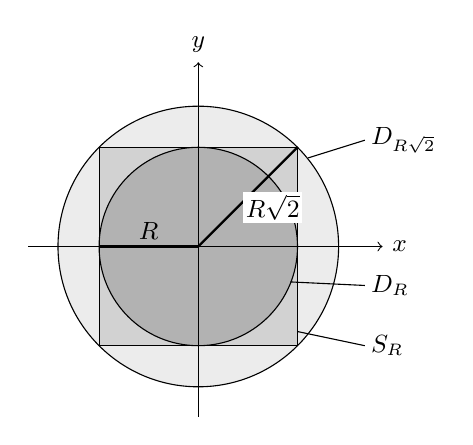
\begin{tikzpicture}[scale=0.9,font=\small]
  \fill[gray!15] (0,0) circle ({1.4*sqrt(2)});
  \fill[gray!35] (-1.4,-1.4) rectangle (1.4,1.4);
  \fill[gray!60] (0,0) circle (1.4);
  \draw (0,0) circle ({1.4*sqrt(2)}); \draw (-1.4,-1.4) rectangle (1.4,1.4); \draw (0,0) circle (1.4);
  \draw[->] (-2.4,0) -- (2.6,0) node[right] {$x$};
  \draw[->] (0,-2.4) -- (0,2.6) node[above] {$y$};
  \draw[thick] (0,0) -- (1.4,1.4);
  \node[fill=white,inner sep=1pt] at (1.05,0.55) {$R\sqrt2$};
  \draw[thick] (0,0) -- (-1.4,0);
  \node[above,fill=gray!60,inner sep=1pt] at (-0.7,0.05) {$R$};
  \node[right] at (2.3,1.5) {$D_{R\sqrt2}$}; \draw (2.35,1.5) -- (1.55,1.25);
  \node[right] at (2.3,-1.4) {$S_R$}; \draw (2.35,-1.4) -- (1.4,-1.2);
  \node[right] at (2.3,-0.55) {$D_R$}; \draw (2.35,-0.55) -- (1.3,-0.5);
\end{tikzpicture}
\caption{El cuadrado $S_R$ contiene al disco $D_R$ y está contenido en $D_{R\sqrt2}$. Las integrales de $e^{-(x^2+y^2)}$ sobre los discos se calculan en polares y encierran a $I(R)^2$.}
\label{fig:t6-gauss}
\end{figure}

\begin{corolario}\label{cor:gauss-normal}
$\displaystyle\int_{-\infty}^{\infty}e^{-x^2/2}\,dx=\sqrt{2\pi}$. En consecuencia, la densidad normal estándar $\varphi(x)=\frac{1}{\sqrt{2\pi}}e^{-x^2/2}$ integra~$1$.
\end{corolario}

\begin{proof}
Con el cambio $x=\sqrt2\,u$, $dx=\sqrt2\,du$: $\int e^{-x^2/2}dx=\sqrt2\int e^{-u^2}du=\sqrt2\sqrt\pi$.
\end{proof}

\begin{observacion}[Errores frecuentes]
\begin{enumerate}[label=(\alph*)]
\item Olvidar el factor $r$ en $dA=r\,dr\,d\theta$. Sin él, el área del disco unidad saldría $2\pi$ en lugar de $\pi$.
\item Poner en la integral exterior límites que dependen de la otra variable: el resultado de una integral doble es un número.
\item Cambiar el orden de integración intercambiando sin más los límites. Hay que redibujar la región y describirla de nuevo (\cref{ej:t6-orden}).
\item Aplicar el \cref{cor:separable} cuando la región no es un rectángulo: sobre un triángulo, $\iint g(x)h(y)\dA$ no es en general el producto de dos integrales.
\end{enumerate}
\end{observacion}

\begin{observacion}[Conexión con el curso]
La distribución normal, omnipresente en el curso (inicialización de los pesos, ruido, teorema central del límite), se define con la densidad del \cref{cor:gauss-normal}; su normalización y el cálculo de su varianza se apoyan en este tema (módulo~5, tema~3, y \cref{eje:6-gaussiana-normal}). Las integrales dobles aparecen también en la entropía diferencial de una normal (módulo~6) y en el cálculo de probabilidades conjuntas de dos variables continuas (módulo~5).
\end{observacion}

\begin{lecturas}
\item MIT 18.02SC~\cite{mit1802}, unidad~3, parte~A, sesiones~47--50 (definición, ejemplos, cambio de orden, polares) y~51 (masa y valor medio).
\item OpenStax \emph{Calculus}, vol.~3~\cite{openstax3}, §5.1 «Double Integrals over Rectangular Regions», §5.2 «Double Integrals over General Regions» y §5.3 «Double Integrals in Polar Coordinates».
\item Apostol~\cite{apostol2}, §11.1--11.14 (integral doble, Fubini, regiones generales) y §11.26--11.31 (cambio de variables).
\item Strang, \emph{Calculus}~\cite{strangcalc}, §14.1 «Double Integrals» y §14.2 «Changing to Better Coordinates».
\end{lecturas}

\section*{Ejercicios del tema 6}
\addcontentsline{toc}{section}{Ejercicios del tema 6}

\begin{ejercicio}{1}{eje:6-simetria}
Sea $D$ el disco unidad centrado en el origen. Sin calcular, decida cuáles de las integrales siguientes son nulas por simetría y, para las demás, escriba una integral equivalente sobre un semidisco o un cuarto de disco: $\iint_Dx\dA$, $\iint_De^x\dA$, $\iint_Dx^2\dA$, $\iint_Dx^2y\dA$, $\iint_D(x^2+y)\dA$, $\iint_Dxy\dA$.
\fuente{adaptado de MIT 18.02SC~\cite{mit1802}, problemas suplementarios, 3A-6.}
\end{ejercicio}

\begin{ejercicio}{2}{eje:6-iteradas}
Calcule: (a) $\displaystyle\int_0^2\int_{-1}^{1}(6x^2+2y)\,dy\,dx$; (b) $\displaystyle\int_0^1\int_0^{u}\sqrt{u^2+4}\,dv\,du$.
\fuente{adaptado de MIT 18.02SC~\cite{mit1802}, problemas suplementarios, 3A-1.}
\end{ejercicio}

\begin{ejercicio}{2}{eje:6-rectangulos}
Calcule sobre los rectángulos indicados: (a) $\iint(x+y)^2\dA$ en $[0,1]\times[0,2]$; (b) $\iint\sin(x+y)\dA$ en $[0,\frac\pi2]\times[0,\frac\pi2]$; (c) $\iint xe^{xy}\dA$ en $[0,1]\times[0,1]$, eligiendo el orden más cómodo.
\fuente{adaptado de OpenStax \emph{Calculus}, vol.~3~\cite{openstax3}, §5.1.}
\end{ejercicio}

\begin{ejercicio}{2}{eje:6-planteo}
Escriba $\iint_Df\dA$ como integral iterada en los dos órdenes, $dy\,dx$ y $dx\,dy$: (a) $D$ es el triángulo de vértices $(0,0)$, $(0,2)$ y $(-2,2)$; (b) $D$ es la región finita comprendida entre la parábola $y=2x-x^2$ y el eje $x$. Calcule el área de la región (b).
\fuente{adaptado de MIT 18.02SC~\cite{mit1802}, problemas suplementarios, 3A-2.}
\end{ejercicio}

\begin{ejercicio}{2}{eje:6-region}
Calcule $\iint_Dx\dA$, donde $D$ es la región limitada por los ejes coordenados y la recta $2y+x=2$.
\fuente{adaptado de MIT 18.02SC~\cite{mit1802}, problemas suplementarios, 3A-3.}
\end{ejercicio}

\begin{ejercicio}{2}{eje:6-volumen-xy}
Halle el volumen del sólido situado bajo la superficie $z=xy$ y sobre la región del primer cuadrante comprendida entre las curvas $y=x$ e $y=x^2$.
\fuente{adaptado de MIT 18.02SC~\cite{mit1802}, problemas suplementarios, 3A-4.}
\end{ejercicio}

\begin{ejercicio}{2}{eje:6-orden-1}
Calcule $\displaystyle\int_0^2\int_x^2e^{-y^2}\,dy\,dx$ cambiando el orden de integración.
\fuente{adaptado de MIT 18.02SC~\cite{mit1802}, problemas suplementarios, 3A-5.}
\end{ejercicio}

\begin{ejercicio}{2}{eje:6-orden-2}
Calcule $\displaystyle\int_0^1\int_{\sqrt[3]{x}}^{1}\frac{1}{1+u^4}\,du\,dx$ cambiando el orden de integración.
\fuente{adaptado de MIT 18.02SC~\cite{mit1802}, problemas suplementarios, 3A-5.}
\end{ejercicio}

\begin{ejercicio}{2}{eje:6-polares}
Calcule, pasando a polares, $\displaystyle\iint_D\frac{dx\,dy}{1+x^2+y^2}$, donde $D$ es la parte del disco $x^2+y^2\le a^2$ situada en el primer cuadrante.
\fuente{adaptado de MIT 18.02SC~\cite{mit1802}, problemas suplementarios, 3B-2.}
\end{ejercicio}

\begin{ejercicio}{2}{eje:6-semiesfera}
Calcule en polares el volumen de una semiesfera maciza de radio $a$, es decir, el volumen bajo $z=\sqrt{a^2-x^2-y^2}$ sobre el disco $x^2+y^2\le a^2$.
\fuente{adaptado de MIT 18.02SC~\cite{mit1802}, problemas suplementarios, 3B-3.}
\end{ejercicio}

\begin{ejercicio}{2}{eje:6-centroide}
El \emph{centroide} de una región $D$ es el punto $(\bar x,\bar y)$ con $\bar x=\frac{1}{\text{área}(D)}\iint_Dx\dA$ e $\bar y$ análogo. Halle el centroide del sector circular de radio $a$ y ángulo central $2\alpha$ ($0<\alpha\le\pi$) colocado simétricamente respecto del eje $x$, con el vértice en el origen. Particularice al semidisco.
\fuente{adaptado de MIT 18.02SC~\cite{mit1802}, problemas suplementarios, 3C-4.}
\end{ejercicio}

\begin{ejercicio}{2}{eje:6-gauss-polar}
(a) Calcule $\iint_{x^2+y^2\le R^2}e^{-(x^2+y^2)}\dA$. (b) ¿Para qué radio $R$ es esa integral el 99\,\% de su valor sobre todo el plano?
\end{ejercicio}

\begin{ejercicio}{3}{eje:6-capas}
Sea $z=f(r)\ge0$ una superficie de revolución alrededor del eje $z$, con $f$ continua en $[0,a]$. (a) Demuestre que la fórmula en polares del volumen bajo la superficie y sobre el disco $r\le a$ coincide con la fórmula de las capas cilíndricas del cálculo de una variable, $V=\int_0^a2\pi r f(r)\,dr$. (b) Aplíquela al cono $f(r)=h(1-r/a)$ y compruebe que se obtiene $\frac13\pi a^2h$.
\fuente{adaptado de MIT 18.02SC~\cite{mit1802}, \emph{problem set}~7, parte~II, problema~2.}
\end{ejercicio}

\begin{ejercicio}{3}{eje:6-cota}
Demuestre, sin calcular la integral, que $\displaystyle\iint_{[0,1]^2}\frac{x}{1+x^2+y^2}\dA<0{,}35$. (Indicación: acote el integrando por una función de $x$ sola y use la monotonía.)
\fuente{adaptado de MIT 18.02SC~\cite{mit1802}, problemas suplementarios, 3A-7.}
\end{ejercicio}

\begin{ejercicio}{3}{eje:6-gaussiana-normal}
(a) Demuestre que $\int_{-\infty}^{\infty}e^{-(x-\mu)^2/(2\sigma^2)}dx=\sigma\sqrt{2\pi}$ para $\mu\in\R$ y $\sigma>0$. (b) Demuestre, integrando por partes, que $\int_{-\infty}^{\infty}x^2e^{-x^2/2}dx=\sqrt{2\pi}$. (c) Deduzca que si $X$ tiene densidad $\varphi(x)=\frac1{\sqrt{2\pi}}e^{-x^2/2}$, entonces $\E[X]=0$ y $\E[X^2]=1$.
\end{ejercicio}


\appendix
% =====================================================================
\chapter{Soluciones de los ejercicios}
\label{ap:soluciones}
% =====================================================================

Cada solución se presenta en cinco partes: datos, planteamiento, desarrollo, resultado y comprobación. En las demostraciones, los datos son las hipótesis, el planteamiento es la estrategia y la comprobación es un caso particular o una verificación independiente. Los valores aproximados se dan con cuatro cifras significativas salvo que se indique otra cosa.

% ---------------------------------------------------------------------
\section{Tema 1}

\begin{solucion}{eje:1-vf}
\datos cinco afirmaciones sobre vectores de $\R^3$.
\planteamiento buscar un contraejemplo o citar el resultado que la demuestra.
\pasos
\begin{enumerate}[label=(\alph*)]
  \item Falsa: $\vu\cdot\vv=\sum u_iv_i$ es un número (\cref{def:escalar}).
  \item Falsa: $\vu=\vi\neq\vcero$ y $\vv=\vj\neq\vcero$ cumplen $\vu\cdot\vv=0$. La condición solo dice que son ortogonales.
  \item Falsa: con $\vu=\vi$ y $\vv=-\vi$, $\norm{\vu+\vv}=0$ y $\norm{\vu}+\norm{\vv}=2$.
  \item Falsa: $\vi\times\vj=\vk$ y $\vj\times\vi=-\vk$ (\cref{prop:vectorial}(i)).
  \item Verdadera: es la \cref{prop:vectorial}(iii).
\end{enumerate}
\resultado \textbf{(a) F; (b) F; (c) F; (d) F; (e) V.}
\comprobacion en (c), la igualdad en la desigualdad triangular exige igualdad en Cauchy--Schwarz con $\vu\cdot\vv\ge0$, es decir, vectores de igual dirección y sentido; $\vi$ y $-\vi$ tienen sentidos opuestos.
\end{solucion}

\begin{solucion}{eje:1-cosenos}
\datos $\va\neq\vcero$ con ángulos $\alpha,\beta,\gamma$ respecto de $\vi,\vj,\vk$; $\va=-\vi+2\vj+2\vk$ en (b).
\planteamiento aplicar la \cref{def:angulo} con los vectores de la base, que son unitarios.
\pasos
\begin{enumerate}[label=\arabic*.]
  \item $\cos\alpha=\dfrac{\va\cdot\vi}{\norm{\va}\norm{\vi}}=\dfrac{a_1}{\norm\va}$, y análogamente $\cos\beta=a_2/\norm\va$, $\cos\gamma=a_3/\norm\va$. Luego $\va/\norm\va=(\cos\alpha,\cos\beta,\cos\gamma)$.
  \item Ese vector es unitario: $\cos^2\alpha+\cos^2\beta+\cos^2\gamma=\norm{\va/\norm\va}^2=1$.
  \item En (b), $\norm\va=\sqrt{1+4+4}=3$, así que $(\cos\alpha,\cos\beta,\cos\gamma)=(-\tfrac13,\tfrac23,\tfrac23)$.
  \item $\alpha=\arccos(-\tfrac13)\approx109{,}47^\circ$ y $\beta=\gamma=\arccos\tfrac23\approx48{,}19^\circ$.
\end{enumerate}
\resultado \textbf{$\va/\norm\va=(\cos\alpha,\cos\beta,\cos\gamma)$; en (b), cosenos $(-\frac13,\frac23,\frac23)$ y ángulos $109{,}47^\circ$, $48{,}19^\circ$, $48{,}19^\circ$.}
\comprobacion $\frac19+\frac49+\frac49=1$. El ángulo con $\vi$ es obtuso porque la primera componente es negativa.
\end{solucion}

\begin{solucion}{eje:1-operaciones}
\datos $\vu=(2,-1,3)$, $\vv=(1,4,-2)$.
\planteamiento operar componente a componente (\cref{def:vector,def:escalar}).
\pasos
\begin{enumerate}[label=\arabic*.]
  \item $\vu+\vv=(3,3,1)$; $3\vu-2\vv=(6-2,\,-3-8,\,9+4)=(4,-11,13)$.
  \item $\vu\cdot\vv=2-4-6=-8$.
  \item $\norm\vu=\sqrt{4+1+9}=\sqrt{14}\approx3{,}742$; $\norm\vv=\sqrt{1+16+4}=\sqrt{21}\approx4{,}583$.
  \item $\vu-\vv=(1,-5,5)$, luego la distancia es $\sqrt{1+25+25}=\sqrt{51}\approx7{,}141$.
  \item Como $\vu\cdot\vv<0$, el ángulo es obtuso.
\end{enumerate}
\resultado \textbf{$(3,3,1)$; $(4,-11,13)$; $-8$; $\sqrt{14}$; $\sqrt{21}$; $\sqrt{51}$; ángulo obtuso.}
\comprobacion por~\eqref{eq:t1-desarrollo}, $\norm{\vu-\vv}^2=14+21-2(-8)=51$.
\end{solucion}

\begin{solucion}{eje:1-unitarios}
\datos tres vectores; en (b), norma 6, dirección $(1,2,-2)/3$ y origen $(-2,0,1)$.
\planteamiento dividir cada vector por su norma; en (b), extremo $=$ origen $+$ vector.
\pasos
\begin{enumerate}[label=\arabic*.]
  \item $\norm{(1,1,1)}=\sqrt3$, unitario $\frac{1}{\sqrt3}(1,1,1)$.
  \item $\norm{(2,-1,2)}=\sqrt{4+1+4}=3$, unitario $\frac13(2,-1,2)$.
  \item $\norm{(3,-6,-2)}=\sqrt{9+36+4}=7$, unitario $\frac17(3,-6,-2)$.
  \item En (b), el vector es $6\cdot\frac13(1,2,-2)=(2,4,-4)$ y el extremo es $(-2,0,1)+(2,4,-4)=(0,4,-3)$.
\end{enumerate}
\resultado \textbf{normas $\sqrt3$, $3$, $7$; unitarios $\frac{(1,1,1)}{\sqrt3}$, $\frac{(2,-1,2)}{3}$, $\frac{(3,-6,-2)}{7}$; extremo $(0,4,-3)$.}
\comprobacion $\norm{(2,4,-4)}=\sqrt{4+16+16}=6$, como se pedía.
\end{solucion}

\begin{solucion}{eje:1-angulos}
\datos (a) $(1,0,-1)$ y $(4,4,-2)$; (b) $(1,1,2)$ y $(2,-1,1)$.
\planteamiento $\cos\theta=\vu\cdot\vv/(\norm\vu\norm\vv)$.
\pasos
\begin{enumerate}[label=\arabic*.]
  \item (a) $\vu\cdot\vv=4+0+2=6$, $\norm\vu=\sqrt2$, $\norm\vv=\sqrt{36}=6$; $\cos\theta=\frac{6}{6\sqrt2}=\frac{1}{\sqrt2}$, $\theta=\pi/4$.
  \item (b) $\vu\cdot\vv=2-1+2=3$, $\norm\vu=\norm\vv=\sqrt6$; $\cos\theta=\frac36=\frac12$, $\theta=\pi/3$.
\end{enumerate}
\resultado \textbf{(a) $45^\circ$; (b) $60^\circ$.}
\comprobacion en (a), $\vu_\perp=\vu-\proj_{\vv}\vu$ tiene norma $\norm\vu\sin45^\circ=1$: $\proj_{\vv}\vu=\frac{6}{36}(4,4,-2)$ y $\vu-\proj_{\vv}\vu=\frac13(1,-2,-2)$, de norma~$1$.
\end{solucion}

\begin{solucion}{eje:1-ortogonal-c}
\datos $\vu=(c,2,-1)$, $\vv=(1,-1,2)$.
\planteamiento el ángulo es recto si $\vu\cdot\vv=0$ y agudo si $\vu\cdot\vv>0$ (\cref{prop:coseno}).
\pasos
\begin{enumerate}[label=\arabic*.]
  \item $\vu\cdot\vv=c-2-2=c-4$.
  \item (a) $c-4=0\iff c=4$. (b) $c-4>0\iff c>4$.
  \item Los vectores nunca son paralelos: $(c,2,-1)=t(1,-1,2)$ exigiría $t=-\frac12$ por la tercera componente y $t=-2$ por la segunda.
\end{enumerate}
\resultado \textbf{(a) $c=4$; (b) $c>4$.}
\comprobacion con $c=4$: $(4,2,-1)\cdot(1,-1,2)=4-2-2=0$.
\end{solucion}

\begin{solucion}{eje:1-proyeccion}
\datos $\mathbf F=(2,-2,1)$, $\va=(3,2,-6)$.
\planteamiento aplicar la \cref{def:proyeccion} y la \cref{prop:descomposicion}.
\pasos
\begin{enumerate}[label=\arabic*.]
  \item $\mathbf F\cdot\va=6-4-6=-4$ y $\norm\va=\sqrt{9+4+36}=7$; la componente escalar es $-\frac47$.
  \item $\proj_{\va}\mathbf F=\frac{-4}{49}(3,2,-6)=\bigl(-\frac{12}{49},-\frac{8}{49},\frac{24}{49}\bigr)$.
  \item $\mathbf F_\perp=\mathbf F-\proj_{\va}\mathbf F=\bigl(\frac{98+12}{49},\frac{-98+8}{49},\frac{49-24}{49}\bigr)=\frac{1}{49}(110,-90,25)$.
\end{enumerate}
\resultado \textbf{componente $-\frac47$; $\mathbf F_\parallel=\frac{1}{49}(-12,-8,24)$; $\mathbf F_\perp=\frac{1}{49}(110,-90,25)$.}
\comprobacion $\mathbf F_\perp\cdot\va=\frac{1}{49}(330-180-150)=0$.
\end{solucion}

\begin{solucion}{eje:1-cubo}
\datos cubo $[0,1]^3$, $P=\vcero$; diagonal principal $(1,1,1)$, diagonal de cara $(1,1,0)$, arista $(1,0,0)$.
\planteamiento \cref{def:angulo}.
\pasos
\begin{enumerate}[label=\arabic*.]
  \item (a) $(1,1,1)\cdot(1,1,0)=2$, normas $\sqrt3$ y $\sqrt2$: $\cos\theta=\frac{2}{\sqrt6}=\sqrt{2/3}$, $\theta\approx35{,}26^\circ$.
  \item (b) $(1,1,1)\cdot(1,0,0)=1$: $\cos\theta=\frac1{\sqrt3}$, $\theta\approx54{,}74^\circ$.
\end{enumerate}
\resultado \textbf{(a) $\arccos\sqrt{2/3}\approx35{,}26^\circ$; (b) $\arccos(1/\sqrt3)\approx54{,}74^\circ$.}
\comprobacion los dos ángulos suman $90^\circ$. La diagonal de cara $(1,1,0)$ es la proyección de $(1,1,1)$ sobre el plano $z=0$, de modo que (a) es el ángulo de la diagonal principal con ese plano, complementario del que forma con $\vk$; y este, por simetría, es igual al de (b). En efecto, $\cos^2$ de uno más $\cos^2$ del otro da $\frac23+\frac13=1$.
\end{solucion}

\begin{solucion}{eje:1-vectorial}
\datos $\va=(1,-2,1)$, $\vb=(2,-1,-1)$; $P=(2,0,1)$, $Q=(3,1,0)$, $R=(-1,1,-1)$.
\planteamiento \cref{def:vectorial}; el área del triángulo es la mitad de $\norm{\overrightarrow{PQ}\times\overrightarrow{PR}}$ (\cref{prop:vectorial}(iv)).
\pasos
\begin{enumerate}[label=\arabic*.]
  \item $\va\times\vb=\bigl((-2)(-1)-1\cdot(-1),\ 1\cdot2-1\cdot(-1),\ 1\cdot(-1)-(-2)\cdot2\bigr)=(3,3,3)$.
  \item $(3,3,3)\cdot\va=3-6+3=0$ y $(3,3,3)\cdot\vb=6-3-3=0$.
  \item $\overrightarrow{PQ}=(1,1,-1)$, $\overrightarrow{PR}=(-3,1,-2)$; su producto vectorial es $\bigl(1\cdot(-2)-(-1)\cdot1,\ (-1)(-3)-1\cdot(-2),\ 1\cdot1-1\cdot(-3)\bigr)=(-1,5,4)$.
  \item $\norm{(-1,5,4)}=\sqrt{1+25+16}=\sqrt{42}$; área $=\frac{\sqrt{42}}{2}\approx3{,}240$.
\end{enumerate}
\resultado \textbf{(a) $(3,3,3)$; (b) $\sqrt{42}/2\approx3{,}240$.}
\comprobacion por la identidad de Lagrange, $\norm{\overrightarrow{PQ}}^2\norm{\overrightarrow{PR}}^2-(\overrightarrow{PQ}\cdot\overrightarrow{PR})^2=3\cdot14-(-3+1+2)^2=42$.
\end{solucion}

\begin{solucion}{eje:1-tetraedro}
\datos $P=(1,0,1)$, $Q=(-1,1,2)$, $R=(0,0,2)$, $S=(3,1,-1)$.
\planteamiento volumen $=\frac16\abs{\overrightarrow{PQ}\cdot(\overrightarrow{PR}\times\overrightarrow{PS})}$ (\cref{prop:volumen}).
\pasos
\begin{enumerate}[label=\arabic*.]
  \item $\overrightarrow{PQ}=(-2,1,1)$, $\overrightarrow{PR}=(-1,0,1)$, $\overrightarrow{PS}=(2,1,-2)$.
  \item $\overrightarrow{PR}\times\overrightarrow{PS}=\bigl(0\cdot(-2)-1\cdot1,\ 1\cdot2-(-1)(-2),\ (-1)\cdot1-0\cdot2\bigr)=(-1,0,-1)$.
  \item $\overrightarrow{PQ}\cdot(-1,0,-1)=2+0-1=1$.
  \item Volumen $=\frac16\cdot1=\frac16$.
\end{enumerate}
\resultado \textbf{$\frac16$.}
\comprobacion desarrollando el determinante de filas $\overrightarrow{PQ},\overrightarrow{PR},\overrightarrow{PS}$ por la primera fila: $-2(0-1)-1(2-2)+1(-1-0)=2-0-1=1$.
\end{solucion}

\begin{solucion}{eje:1-polarizacion}
\datos $\vu,\vv\in\R^n$; en (b), no nulos y no opuestos.
\planteamiento (a) usar~\eqref{eq:t1-desarrollo}; (b) comparar los cosenos de los dos ángulos.
\pasos
\begin{enumerate}[label=\arabic*.]
  \item Por~\eqref{eq:t1-desarrollo}, $\norm{\vu+\vv}^2-\norm{\vu-\vv}^2=(\norm\vu^2+2\vu\cdot\vv+\norm\vv^2)-(\norm\vu^2-2\vu\cdot\vv+\norm\vv^2)=4\,\vu\cdot\vv$. Dividiendo por~4 se obtiene la identidad.
  \item $\vw=\hat\vu+\hat\vv\neq\vcero$, porque $\hat\vu=-\hat\vv$ significaría que $\vu$ y $\vv$ tienen sentidos opuestos.
  \item $\vw\cdot\hat\vu=1+\hat\vu\cdot\hat\vv$ y $\vw\cdot\hat\vv=\hat\vu\cdot\hat\vv+1$, iguales.
  \item El coseno del ángulo entre $\vw$ y $\vu$ es $\vw\cdot\hat\vu/\norm\vw$, y el del ángulo entre $\vw$ y $\vv$ es $\vw\cdot\hat\vv/\norm\vw$; son iguales, y como $\arccos$ es inyectiva en $[-1,1]$, los ángulos coinciden.
\end{enumerate}
\resultado \textbf{$\vu\cdot\vv=\frac14\norm{\vu+\vv}^2-\frac14\norm{\vu-\vv}^2$; el bisector unitario es $(\hat\vu+\hat\vv)/\norm{\hat\vu+\hat\vv}$.}
\comprobacion con $\vu=\vi$, $\vv=3\vj$: $\hat\vu+\hat\vv=(1,1,0)$ forma $45^\circ$ con ambos. Y $\frac14(10)-\frac14(10)=0=\vu\cdot\vv$.
\end{solucion}

\begin{solucion}{eje:1-cs-cuadratica}
\datos $\vu,\vv\in\R^n$, $\vv\neq\vcero$ (si $\vv=\vcero$ la desigualdad es trivial).
\planteamiento un polinomio de grado~2 con coeficiente principal positivo que no toma valores negativos tiene discriminante menor o igual que cero.
\pasos
\begin{enumerate}[label=\arabic*.]
  \item (a) $p(t)=\norm{\vu+t\vv}^2\ge0$ por la positividad del producto escalar.
  \item (b) Por~\eqref{eq:t1-desarrollo} con $t\vv$: $p(t)=\norm\vv^2t^2+2(\vu\cdot\vv)t+\norm\vu^2$, con coeficiente principal $\norm\vv^2>0$.
  \item (c) Si el discriminante fuera positivo, $p$ tendría dos raíces reales distintas y sería negativo entre ellas. Luego $4(\vu\cdot\vv)^2-4\norm\vu^2\norm\vv^2\le0$, es decir, $\abs{\vu\cdot\vv}\le\norm\vu\norm\vv$.
  \item (d) La igualdad equivale a discriminante nulo, es decir, a que $p$ tenga una raíz (doble) $t_0$: $\norm{\vu+t_0\vv}=0$, o sea, $\vu=-t_0\vv$.
\end{enumerate}
\resultado \textbf{$\abs{\vu\cdot\vv}\le\norm\vu\norm\vv$, con igualdad si y solo si $\vu$ es múltiplo de $\vv$.}
\comprobacion con $\vu=(1,2)$, $\vv=(2,4)$: $p(t)=20t^2+20t+5=5(2t+1)^2$, que tiene la raíz doble $t_0=-\frac12$, y $\vu=\frac12\vv$.
\end{solucion}

\begin{solucion}{eje:1-rombo}
\datos paralelogramo de lados (como vectores) $\va$ y $\vb$.
\planteamiento las diagonales son $\va+\vb$ y $\va-\vb$; calcular su producto escalar.
\pasos
\begin{enumerate}[label=\arabic*.]
  \item Con un vértice en el origen, los otros son $\va$, $\vb$ y $\va+\vb$. Las diagonales son $\va+\vb$ (del origen al vértice opuesto) y $\va-\vb$ (de $\vb$ a $\va$).
  \item $(\va+\vb)\cdot(\va-\vb)=\norm\va^2-\va\cdot\vb+\vb\cdot\va-\norm\vb^2=\norm\va^2-\norm\vb^2$.
  \item Por tanto, las diagonales son perpendiculares si y solo si $\norm\va=\norm\vb$.
  \item En un paralelogramo los lados opuestos son iguales; $\norm\va=\norm\vb$ equivale a que los cuatro lados sean iguales.
\end{enumerate}
\resultado \textbf{diagonales perpendiculares $\iff\norm\va=\norm\vb\iff$ rombo.}
\comprobacion para el rombo de lados $\va=(2,0)$, $\vb=(1,\sqrt3)$, las diagonales $(3,\sqrt3)$ y $(1,-\sqrt3)$ cumplen $3-3=0$.
\end{solucion}

\begin{solucion}{eje:1-semicirculo}
\datos circunferencia de centro $O$ y radio $\rho$; $A$, $B$ extremos de un diámetro; $C$ otro punto de la circunferencia.
\planteamiento escribir todo respecto de $O$ y calcular $\overrightarrow{CA}\cdot\overrightarrow{CB}$.
\pasos
\begin{enumerate}[label=\arabic*.]
  \item Sean $\va=\overrightarrow{OA}$ y $\mathbf c=\overrightarrow{OC}$; entonces $\overrightarrow{OB}=-\va$ y $\norm\va=\norm{\mathbf c}=\rho$.
  \item $\overrightarrow{CA}=\va-\mathbf c$ y $\overrightarrow{CB}=-\va-\mathbf c$; ambos son no nulos porque $C\neq A,B$.
  \item $(\va-\mathbf c)\cdot(-\va-\mathbf c)=-\norm\va^2-\va\cdot\mathbf c+\mathbf c\cdot\va+\norm{\mathbf c}^2=\rho^2-\rho^2=0$.
\end{enumerate}
\resultado \textbf{$\overrightarrow{CA}\cdot\overrightarrow{CB}=0$: el ángulo en $C$ es recto.}
\comprobacion con la circunferencia unidad, $A=(1,0)$, $B=(-1,0)$, $C=(0,1)$: $(1,-1)\cdot(-1,-1)=-1+1=0$.
\end{solucion}

\begin{solucion}{eje:1-lagrange-id}
\datos $\vu,\vv\in\R^3$.
\planteamiento desarrollar ambos miembros y agrupar por pares de índices $i<j$.
\pasos
\begin{enumerate}[label=\arabic*.]
  \item Miembro izquierdo: $(u_2v_3-u_3v_2)^2+(u_3v_1-u_1v_3)^2+(u_1v_2-u_2v_1)^2=\sum_{i<j}(u_iv_j-u_jv_i)^2$, una suma sobre los tres pares $(1,2),(1,3),(2,3)$.
  \item Miembro derecho: $\bigl(\sum_iu_i^2\bigr)\bigl(\sum_jv_j^2\bigr)-\bigl(\sum_iu_iv_i\bigr)^2=\sum_{i,j}u_i^2v_j^2-\sum_iu_i^2v_i^2-2\sum_{i<j}u_iv_iu_jv_j$.
  \item Los términos con $i=j$ se cancelan y queda $\sum_{i\neq j}u_i^2v_j^2-2\sum_{i<j}u_iv_iu_jv_j=\sum_{i<j}\bigl(u_i^2v_j^2+u_j^2v_i^2-2u_iv_ju_jv_i\bigr)=\sum_{i<j}(u_iv_j-u_jv_i)^2$.
  \item (b) $\vu\times\vv=\vcero\iff\norm{\vu\times\vv}^2=0\iff(\vu\cdot\vv)^2=\norm\vu^2\norm\vv^2$, que es el caso de igualdad de Cauchy--Schwarz (\cref{teo:cs}): uno es múltiplo del otro.
\end{enumerate}
\resultado \textbf{$\norm{\vu\times\vv}^2=\norm\vu^2\norm\vv^2-(\vu\cdot\vv)^2$; $\vu\times\vv=\vcero$ si y solo si $\vu$ y $\vv$ son paralelos.}
\comprobacion con $\va=(1,-2,1)$, $\vb=(2,-1,-1)$ del \cref{eje:1-vectorial}: $\norm{(3,3,3)}^2=27$ y $6\cdot6-3^2=27$.
\end{solucion}

% ---------------------------------------------------------------------
\section{Tema 2}

\begin{solucion}{eje:2-posicion}
\datos tres pares de planos.
\planteamiento aplicar la \cref{prop:dos-planos}: comparar normales y, si son proporcionales, los términos independientes.
\pasos
\begin{enumerate}[label=(\alph*)]
  \item $(2,4,-2)=2(1,2,-1)$, pero $5\neq2\cdot1$: planos paralelos distintos; sistema incompatible.
  \item $(3,6,-3)=3(1,2,-1)$ y $3=3\cdot1$: el mismo plano; sistema compatible indeterminado (las soluciones forman un plano).
  \item $(1,1,0)$ y $(0,1,1)$ no son proporcionales: se cortan en una recta de dirección $(1,1,0)\times(0,1,1)=(1,-1,1)$; sistema compatible indeterminado.
\end{enumerate}
\resultado \textbf{(a) paralelos, incompatible; (b) coincidentes, indeterminado; (c) se cortan en una recta, indeterminado.}
\comprobacion en (c), el punto $(1,0,1)$ está en ambos planos y $(1,0,1)+t(1,-1,1)$ cumple $x+y=1$ e $y+z=1$ para todo $t$.
\end{solucion}

\begin{solucion}{eje:2-planos}
\datos (a) $P_0=(2,0,-1)$, $\vn=(1,2,-2)$; (b) $P=(1,0,1)$, $Q=(2,-1,2)$, $R=(-1,3,2)$.
\planteamiento \cref{def:plano}; en (b), $\vn=\overrightarrow{PQ}\times\overrightarrow{PR}$.
\pasos
\begin{enumerate}[label=\arabic*.]
  \item (a) $d=\vn\cdot P_0=2+0+2=4$: el plano es $x+2y-2z=4$.
  \item (b) $\overrightarrow{PQ}=(1,-1,1)$, $\overrightarrow{PR}=(-2,3,1)$; $\vn=\bigl((-1)\cdot1-1\cdot3,\ 1\cdot(-2)-1\cdot1,\ 1\cdot3-(-1)(-2)\bigr)=(-4,-3,1)$.
  \item $d=\vn\cdot P=-4+0+1=-3$: $-4x-3y+z=-3$, es decir, $4x+3y-z=3$.
\end{enumerate}
\resultado \textbf{(a) $x+2y-2z=4$; (b) $4x+3y-z=3$.}
\comprobacion en (b): $Q$ da $8-3-2=3$ y $R$ da $-4+9-2=3$.
\end{solucion}

\begin{solucion}{eje:2-diedro}
\datos normales $\vn_1=(2,-1,1)$ y $\vn_2=(1,1,2)$.
\planteamiento el ángulo entre planos es el de sus normales (\cref{prop:dos-planos}).
\pasos
\begin{enumerate}[label=\arabic*.]
  \item $\vn_1\cdot\vn_2=2-1+2=3$; $\norm{\vn_1}=\norm{\vn_2}=\sqrt6$.
  \item $\cos\varphi=\frac36=\frac12$, luego $\varphi=\frac\pi3$.
\end{enumerate}
\resultado \textbf{$60^\circ$.}
\comprobacion la recta de intersección tiene dirección $\vn_1\times\vn_2=(-3,-3,3)$, ortogonal a ambas normales: $-6+3+3=0$ y $-3-3+6=0$.
\end{solucion}

\begin{solucion}{eje:2-interseccion}
\datos (a) punto $(2,-1,-1)$, plano $x-y+2z=3$; (b) recta por $(0,1,2)$ y $(2,0,3)$, plano $x+4y+z=4$.
\planteamiento (a) la normal del plano es el vector director; (b) sustituir la paramétrica en el plano.
\pasos
\begin{enumerate}[label=\arabic*.]
  \item (a) $\vr(t)=(2,-1,-1)+t(1,-1,2)=(2+t,\,-1-t,\,-1+2t)$.
  \item (b) Vector director $(2,0,3)-(0,1,2)=(2,-1,1)$; recta $(2t,\,1-t,\,2+t)$.
  \item Sustituyendo: $2t+4(1-t)+(2+t)=4$, es decir, $6-t=4$, $t=2$.
  \item Punto: $(4,-1,4)$.
\end{enumerate}
\resultado \textbf{(a) $(2+t,-1-t,-1+2t)$; (b) $(4,-1,4)$.}
\comprobacion $4+4(-1)+4=4$; además $(4,-1,4)=(0,1,2)+2(2,-1,1)$ está en la recta.
\end{solucion}

\begin{solucion}{eje:2-gauss}
\datos $x_1-x_2+x_3=2$, $x_2+x_3=0$, $-x_1-x_2+2x_3=3$.
\planteamiento escalonar la matriz ampliada con operaciones (E3) y sustituir hacia atrás; el determinante es el producto de la diagonal final.
\pasos
\begin{enumerate}[label=\arabic*.]
  \item $F_3+F_1$: la tercera fila pasa a $(0,-2,3\mid5)$.
  \item $F_3+2F_2$: $(0,0,5\mid5)$.
  \item $x_3=1$; $x_2=-x_3=-1$; $x_1=2+x_2-x_3=0$.
  \item Solo se han usado operaciones (E3), luego $\det A=1\cdot1\cdot5=5$.
\end{enumerate}
\resultado \textbf{$(x_1,x_2,x_3)=(0,-1,1)$; $\det A=5$.}
\comprobacion $0+1+1=2$, $-1+1=0$, $0+1+2=3$. Desarrollo directo: $1(2+1)+1(0+1)+1(0+1)=5$.
\end{solucion}

\begin{solucion}{eje:2-gauss-casos}
\datos tres sistemas $3\times3$.
\planteamiento eliminación gaussiana (\cref{sec:t2-gauss}).
\pasos
\begin{enumerate}[label=\arabic*.]
  \item (a) $F_2-2F_1\to(0,-3,-1\mid-9)$; $F_3-F_1\to(0,1,-2\mid-4)$; $F_3+\frac13F_2\to(0,0,-\frac73\mid-7)$. Luego $z=3$, $-3y-3=-9\Rightarrow y=2$, $x=6-2-3=1$.
  \item (b) $F_2-F_1\to(0,1,2\mid1)$; $F_3-2F_1\to(0,1,2\mid1)$; $F_3-F_2\to(0,0,0\mid0)$. Con $z$ libre: $y=1-2z$, $x=1-y-z=z$.
  \item (c) Las mismas operaciones llevan la última fila a $(0,0,0\mid1)$: $0=1$, imposible.
\end{enumerate}
\resultado \textbf{(a) compatible determinado, $(1,2,3)$: tres planos con un punto común. (b) compatible indeterminado, $(z,1-2z,z)$: los tres planos comparten una recta. (c) incompatible: los planos se cortan dos a dos en rectas paralelas, sin punto común a los tres.}
\comprobacion (a) $1+2+3=6$, $2-2+3=3$, $1+4-3=2$. (b) con $z=1$, $(1,-1,1)$: $1$, $1-2+3=2$, $2-3+4=3$.
\end{solucion}

\begin{solucion}{eje:2-parametro}
\datos sistema homogéneo con matriz de filas $(1,-1,1)$, $(2,1,1)$, $(-1,c,2)$.
\planteamiento un sistema $3\times3$ homogéneo tiene soluciones no triviales si y solo si $\det A=0$.
\pasos
\begin{enumerate}[label=\arabic*.]
  \item $\det A=1(2-c)-(-1)(4+1)+1(2c+1)=2-c+5+2c+1=c+8$; se anula para $c=-8$.
  \item $\vw=(1,-1,1)\times(2,1,1)=\bigl(-1-1,\ 2-1,\ 1+2\bigr)=(-2,1,3)$ es ortogonal a las dos primeras filas, luego cumple las dos primeras ecuaciones.
  \item Con $c=-8$ las tres filas son coplanarias (\cref{prop:volumen}): la tercera es combinación de las dos primeras, $(-1,-8,2)=5(1,-1,1)-3(2,1,1)$, y por tanto también es ortogonal a $\vw$.
\end{enumerate}
\resultado \textbf{$c=-8$; solución no trivial $(-2,1,3)$ (y sus múltiplos).}
\comprobacion $(-1)(-2)+(-8)(1)+2\cdot3=2-8+6=0$.
\end{solucion}

\begin{solucion}{eje:2-areas}
\datos los triángulos de vértices indicados.
\planteamiento área $=\frac12\abs{\det(\overrightarrow{P_1P_2},\overrightarrow{P_1P_3})}$ (\cref{teo:det-area}).
\pasos
\begin{enumerate}[label=\arabic*.]
  \item (a) Vectores $(1,2)$ y $(1,-1)$: $\det=1\cdot(-1)-2\cdot1=-3$; área $\frac32$.
  \item (b) Desde $(1,2)$: $(0,-3)$ y $(1,1)$; $\det=0\cdot1-(-3)\cdot1=3$; área $\frac32$.
\end{enumerate}
\resultado \textbf{(a) $\frac32$; (b) $\frac32$.}
\comprobacion (a) con base el lado vertical de $(1,2)$ a $(1,-1)$, de longitud $3$, y altura la distancia de $(0,0)$ a la recta $x=1$, que es $1$: $\frac12\cdot3\cdot1=\frac32$.
\end{solucion}

\begin{solucion}{eje:2-inversa}
\datos $A=\begin{pmatrix}4&3\\3&2\end{pmatrix}$, $\vb=(2,3)$.
\planteamiento fórmula~\eqref{eq:t2-inversa} y $\vx=A^{-1}\vb$.
\pasos
\begin{enumerate}[label=\arabic*.]
  \item $\det A=8-9=-1$; $A^{-1}=-1\cdot\begin{pmatrix}2&-3\\-3&4\end{pmatrix}=\begin{pmatrix}-2&3\\3&-4\end{pmatrix}$.
  \item $AA^{-1}=\begin{pmatrix}-8+9&12-12\\-6+6&9-8\end{pmatrix}=I$.
  \item $\vx=A^{-1}\vb=(-4+9,\ 6-12)=(5,-6)$.
\end{enumerate}
\resultado \textbf{$A^{-1}=\begin{pmatrix}-2&3\\3&-4\end{pmatrix}$, $\vx=(5,-6)$.}
\comprobacion $4\cdot5+3(-6)=2$ y $3\cdot5+2(-6)=3$.
\end{solucion}

\begin{solucion}{eje:2-produccion}
\datos columnas de consumo $(1,2,3)$, $(1,3,5)$, $(3,5,8)$; $\vb=(137,279,448)$.
\planteamiento la fila $i$ del sistema cuenta el consumo de $M_i$: $A=\begin{pmatrix}1&1&3\\2&3&5\\3&5&8\end{pmatrix}$, $A\vx=\vb$.
\pasos
\begin{enumerate}[label=\arabic*.]
  \item $\det A=1(24-25)-1(16-15)+3(10-9)=-1-1+3=1\neq0$: solución única.
  \item Eliminación: $F_2-2F_1\to(0,1,-1\mid5)$, $F_3-3F_1\to(0,2,-1\mid37)$, $F_3-2F_2\to(0,0,1\mid27)$.
  \item $x_3=27$, $x_2=5+27=32$, $x_1=137-32-3\cdot27=24$.
  \item (c) Con la columna $(2,5,8)=(1,2,3)+(1,3,5)$, $\det A=1(24-25)-1(16-15)+2(10-9)=0$.
  \item Entonces $A\vx$ siempre está en el plano generado por $(1,2,3)$ y $(1,3,5)$, de normal $(1,2,3)\times(1,3,5)=(1,-2,1)$. Como $(1,-2,1)\cdot\vb=137-558+448=27\neq0$, el sistema es incompatible.
\end{enumerate}
\resultado \textbf{(a) $\det A=1$; (b) $24$, $32$ y $27$ unidades de $P_1$, $P_2$, $P_3$; (c) $\det A=0$ y los consumos dados serían imposibles.}
\comprobacion $24+32+81=137$, $48+96+135=279$, $72+160+216=448$.
\end{solucion}

\begin{solucion}{eje:2-cramer}
\datos $A=\begin{pmatrix}3&-1&1\\-1&2&1\\1&-1&1\end{pmatrix}$, $\vb=(1,2,-3)$.
\planteamiento la incógnita $j$ es $\det A_j/\det A$, donde $A_j$ es $A$ con la columna $j$ sustituida por $\vb$.
\pasos
\begin{enumerate}[label=\arabic*.]
  \item $\det A=3(2+1)-(-1)(-1-1)+1(1-2)=9-2-1=6$.
  \item $\det A_1=\begin{vmatrix}1&-1&1\\2&2&1\\-3&-1&1\end{vmatrix}=1(2+1)+1(2+3)+1(-2+6)=12$, luego $x=2$.
  \item $\det A_2=\begin{vmatrix}3&1&1\\-1&2&1\\1&-3&1\end{vmatrix}=3(2+3)-1(-1-1)+1(3-2)=18$, luego $y=3$.
  \item $\det A_3=\begin{vmatrix}3&-1&1\\-1&2&2\\1&-1&-3\end{vmatrix}=3(-6+2)+1(3-2)+1(1-2)=-12$, luego $z=-2$.
\end{enumerate}
\resultado \textbf{$(x,y,z)=(2,3,-2)$.}
\comprobacion $6-3-2=1$, $-2+6-2=2$, $2-3-2=-3$.
\end{solucion}

\begin{solucion}{eje:2-distancia}
\datos $P_1=(x_1,y_1,z_1)$; plano $\vn\cdot X=d$ con $\vn=(a,b,c)\neq\vcero$.
\planteamiento descomponer $\overrightarrow{P_0P_1}$ en sus partes normal y paralela al plano (\cref{prop:descomposicion}).
\pasos
\begin{enumerate}[label=\arabic*.]
  \item Sea $P_0$ un punto del plano ($\vn\cdot P_0=d$). Para cualquier $X$ del plano, $X-P_0\perp\vn$.
  \item Sea $\mathbf p=\overrightarrow{P_0P_1}=\mathbf p_\parallel+\mathbf p_\perp$ con $\mathbf p_\parallel=\proj_{\vn}\mathbf p$. Entonces $P_1-X=\mathbf p_\parallel+(\mathbf p_\perp-(X-P_0))$, suma de un múltiplo de $\vn$ y de un vector ortogonal a $\vn$.
  \item Por Pitágoras, $\norm{P_1-X}^2=\norm{\mathbf p_\parallel}^2+\norm{\mathbf p_\perp-(X-P_0)}^2\ge\norm{\mathbf p_\parallel}^2$, con igualdad para $X=P_0+\mathbf p_\perp$, que está en el plano.
  \item La distancia es $\norm{\mathbf p_\parallel}=\dfrac{\abs{\vn\cdot(P_1-P_0)}}{\norm\vn}=\dfrac{\abs{ax_1+by_1+cz_1-d}}{\sqrt{a^2+b^2+c^2}}$.
  \item (b) Con $P_1=\vcero$: $\abs d/\norm\vn$. Para $(1,2,3)$ y $2x-y+2z=10$: $\abs{2-2+6-10}/\sqrt{9}=\frac43$.
\end{enumerate}
\resultado \textbf{$d(P_1,\Pi)=\frac{\abs{ax_1+by_1+cz_1-d}}{\sqrt{a^2+b^2+c^2}}$; del origen, $\frac{\abs d}{\norm\vn}$; en el ejemplo, $\frac43$.}
\comprobacion el pie de la perpendicular es $(1,2,3)+\frac49(2,-1,2)=(\frac{17}9,\frac{14}9,\frac{35}9)$, que cumple $\frac{34-14+70}{9}=10$, y está a distancia $\frac49\cdot3=\frac43$.
\end{solucion}

\begin{solucion}{eje:2-vandermonde}
\datos $V=\begin{pmatrix}1&1&1\\x_1&x_2&x_3\\x_1^2&x_2^2&x_3^2\end{pmatrix}$.
\planteamiento restar la primera columna a las otras dos (operación que no cambia el determinante, por la \cref{prop:det-propiedades}(iii) y (iv)) y desarrollar por la primera fila.
\pasos
\begin{enumerate}[label=\arabic*.]
  \item Tras $C_2-C_1$ y $C_3-C_1$, la primera fila es $(1,0,0)$, y $\det V=\begin{vmatrix}x_2-x_1&x_3-x_1\\x_2^2-x_1^2&x_3^2-x_1^2\end{vmatrix}$.
  \item Sacando los factores: $\det V=(x_2-x_1)(x_3-x_1)\begin{vmatrix}1&1\\x_2+x_1&x_3+x_1\end{vmatrix}=(x_2-x_1)(x_3-x_1)(x_3-x_2)$.
  \item Como $(x_1-x_2)(x_2-x_3)=(x_2-x_1)(x_3-x_2)$ (dos cambios de signo), $\det V=(x_1-x_2)(x_2-x_3)(x_3-x_1)$.
  \item La parábola debe cumplir $c_0+c_1x_i+c_2x_i^2=y_i$, $i=1,2,3$: un sistema cuya matriz es $V^{\mathsf T}$, con $\det V^{\mathsf T}=\det V\neq0$ si los $x_i$ son distintos. Por la regla de Cramer en orden~3, la solución existe y es única.
\end{enumerate}
\resultado \textbf{$\det V=(x_1-x_2)(x_2-x_3)(x_3-x_1)$; la parábola por tres puntos de abscisas distintas es única.}
\comprobacion con $(x_1,x_2,x_3)=(0,1,2)$: fórmula, $(-1)(-1)(2)=2$; directamente, $\begin{vmatrix}1&1&1\\0&1&2\\0&1&4\end{vmatrix}=4-2=2$.
\end{solucion}

\begin{solucion}{eje:2-compatibilidad}
\datos $a_1b_2-a_2b_1=0$, $a_1\neq0$.
\planteamiento eliminar $x$ de la segunda ecuación.
\pasos
\begin{enumerate}[label=\arabic*.]
  \item $F_2-\frac{a_2}{a_1}F_1$ da $\bigl(b_2-\frac{a_2b_1}{a_1}\bigr)y=c_2-\frac{a_2}{a_1}c_1$.
  \item El coeficiente de $y$ es $\frac{a_1b_2-a_2b_1}{a_1}=0$, de modo que la ecuación es $0=c_2-\frac{a_2}{a_1}c_1$.
  \item Si $c_2\neq\frac{a_2}{a_1}c_1$, es una contradicción: incompatible. Si $c_2=\frac{a_2}{a_1}c_1$, es $0=0$ y el sistema equivale (\cref{prop:elementales}) a $a_1x+b_1y=c_1$.
  \item Esa ecuación tiene infinitas soluciones: $y=s$ libre y $x=(c_1-b_1s)/a_1$.
\end{enumerate}
\resultado \textbf{compatible $\iff c_2=\frac{a_2}{a_1}c_1$, y entonces con infinitas soluciones (una recta).}
\comprobacion $x+2y=3$, $2x+4y=6$: $c_2=6=2\cdot3$, compatible ($(1,1)$, $(3,0)$, \dots); con $c_2=7$ no hay solución.
\end{solucion}

\begin{solucion}{eje:2-producto-det}
\datos $A=\begin{pmatrix}a&b\\c&d\end{pmatrix}$, $B=\begin{pmatrix}e&f\\g&h\end{pmatrix}$.
\planteamiento (a) cálculo directo; (b) comprobar la definición de inversa; (c) aplicar (a) a $AA^{-1}=I$.
\pasos
\begin{enumerate}[label=\arabic*.]
  \item $AB=\begin{pmatrix}ae+bg&af+bh\\ce+dg&cf+dh\end{pmatrix}$.
  \item $\det(AB)=(ae+bg)(cf+dh)-(af+bh)(ce+dg)$. Los términos $aecf$, $bgdh$ se cancelan con $afce$, $bhdg$, y quedan $aedh+bgcf-afdg-bhce=ad(eh-fg)-bc(eh-fg)=(ad-bc)(eh-fg)$.
  \item (b) $(AB)(B^{-1}A^{-1})=A(BB^{-1})A^{-1}=AIA^{-1}=AA^{-1}=I$, y análogamente $(B^{-1}A^{-1})(AB)=B^{-1}(A^{-1}A)B=I$, usando la asociatividad del producto de matrices.
  \item (c) $\det A\cdot\det(A^{-1})=\det(AA^{-1})=\det I=1$.
\end{enumerate}
\resultado \textbf{$\det(AB)=\det A\det B$; $(AB)^{-1}=B^{-1}A^{-1}$; $\det(A^{-1})=1/\det A$.}
\comprobacion con la matriz del \cref{eje:2-inversa}, $\det A=-1$ y $\det A^{-1}=(-2)(-4)-9=-1=1/(-1)$.
\end{solucion}

% ---------------------------------------------------------------------
\section{Tema 3}

\begin{solucion}{eje:3-conceptos}
\datos tres afirmaciones.
\planteamiento aplicar las definiciones y los ejemplos del tema.
\pasos
\begin{enumerate}[label=(\alph*)]
  \item Falsa: un punto común a los niveles $c_1\neq c_2$ tendría dos valores de $f$.
  \item Falsa: $g(x,y)=\frac{x^2y}{x^4+y^2}$ tiende a~0 por todas las rectas y vale $\frac12$ sobre $y=x^2$ (\cref{ej:t3-no-existe}).
  \item Verdadera: la gráfica son los puntos $(x,y,f(x,y))$ y las curvas de nivel, puntos $(x,y)$ del dominio.
\end{enumerate}
\resultado \textbf{(a) F; (b) F; (c) V.}
\comprobacion el \cref{teo:trayectorias} solo da una condición necesaria, lo que explica (b).
\end{solucion}

\begin{solucion}{eje:3-dominios}
\datos cuatro fórmulas.
\planteamiento raíz: radicando $\ge0$; logaritmo: argumento $>0$; cociente: denominador $\neq0$.
\pasos
\begin{enumerate}[label=(\alph*)]
  \item $x^2+y^2\le1$: disco unidad cerrado. Imagen $[0,1]$ (máximo $1$ en el origen, $0$ en el borde).
  \item $x>y$: semiplano abierto por debajo de la recta $y=x$. Imagen $\R$: sobre $y=0$, $\ln x$ toma todos los valores reales.
  \item $xy\neq0$: el plano sin los dos ejes. Imagen $\R\setminus\{0\}$: con $x=1$, $y=1/k$ se obtiene cualquier $k\neq0$.
  \item $y\ge x^2$: la región sobre la parábola, incluida esta. Imagen $[0,\infty)$: con $x=0$, $\sqrt y$ recorre $[0,\infty)$.
\end{enumerate}
\resultado \textbf{(a) disco cerrado, $[0,1]$; (b) $\{x>y\}$, $\R$; (c) $\{xy\neq0\}$, $\R\setminus\{0\}$; (d) $\{y\ge x^2\}$, $[0,\infty)$.}
\comprobacion (a) $(0{,}6;0{,}8)$ está en el borde y da $\sqrt{1-1}=0$.
\end{solucion}

\begin{solucion}{eje:3-niveles}
\datos cuatro funciones y sus niveles.
\planteamiento resolver $f(x,y)=c$ para cada $c$.
\pasos
\begin{enumerate}[label=(\alph*)]
  \item $1-x-y=c\iff x+y=1-c$: rectas paralelas $x+y=2$, $x+y=1$, $x+y=0$. La gráfica es un plano.
  \item $x^2+y^2=c$: el origen ($c=0$) y circunferencias de radios $1$ y $2$. Paraboloide de vértice el origen, abierto hacia arriba.
  \item $1-x^2-y^2=c\iff x^2+y^2=1-c$: el origen ($c=1$), la circunferencia unidad ($c=0$) y la de radio~$2$ ($c=-3$). Paraboloide abierto hacia abajo con vértice $(0,0,1)$.
  \item $x^2-y^2=1$: hipérbola con vértices $(\pm1,0)$; $c=0$: rectas $y=\pm x$; $c=-1$: hipérbola $y^2-x^2=1$ con vértices $(0,\pm1)$. Silla de montar.
\end{enumerate}
\resultado \textbf{rectas paralelas (plano); circunferencias (paraboloide); circunferencias (paraboloide invertido); hipérbolas y asíntotas (silla).}
\comprobacion (c) $(2,0)$ da $1-4=-3$ y (d) $(1,0)$ da $1$.
\end{solucion}

\begin{solucion}{eje:3-niveles-2}
\datos $f=x^2+4y^2$, $g=y-x^2$, $h=2x+y$, $F=x^2+y^2+z^2$.
\planteamiento identificar la cónica o cuádrica de $f=c$.
\pasos
\begin{enumerate}[label=(\alph*)]
  \item $c>0$: $\frac{x^2}{c}+\frac{y^2}{c/4}=1$, elipses de semiejes $\sqrt c$ y $\sqrt c/2$; $c=0$: el origen; $c<0$: vacío.
  \item $y=x^2+c$: parábolas trasladadas verticalmente.
  \item $2x+y=c$: rectas paralelas de normal $(2,1)$, el vector de coeficientes (\cref{tema:2}). Dos niveles consecutivos $c$ y $c+1$ distan $1/\sqrt5$.
  \item $c>0$: esferas de radio $\sqrt c$ centradas en el origen; $c=0$: el origen.
\end{enumerate}
\resultado \textbf{elipses; parábolas; rectas de normal $(2,1)$; esferas.}
\comprobacion (a) $(\sqrt c,0)$ y $(0,\sqrt c/2)$ dan $c$; (c) la distancia entre $2x+y=c$ y $2x+y=c+1$ es $1/\norm{(2,1)}$ por el \cref{eje:2-distancia}.
\end{solucion}

\begin{solucion}{eje:3-onda}
\datos $F(x,t)=\cos^2(x-ct)$.
\planteamiento $F$ depende solo de $u=x-ct$.
\pasos
\begin{enumerate}[label=\arabic*.]
  \item (a) $F=k$ con $0<k<1$ equivale a $u\in\{\pm\arccos\sqrt k+n\pi:n\in\Z\}$; cada valor $u_0$ da la recta $x-ct=u_0$, es decir, $t=(x-u_0)/c$. Las curvas de nivel son rectas paralelas de pendiente $1/c$ en el plano $(x,t)$.
  \item (b) $F(x,t)=F(x-ct,0)$: la gráfica en el instante $t$ es la del instante~0 trasladada $ct$ hacia la derecha. Con $c=2$ y $t=-1,0,1$, la misma curva $\cos^2x$ aparece desplazada $-2$, $0$ y $2$ unidades.
  \item El perfil se desplaza sin deformarse con velocidad $c$: es una \emph{onda viajera}.
\end{enumerate}
\resultado \textbf{niveles: rectas $x-ct=\text{cte}$; $F$ describe una onda que viaja hacia la derecha con velocidad $c$.}
\comprobacion los máximos ($F=1$) están en $x-2t=n\pi$; en $t=1$, uno de ellos está en $x=2$, dos unidades a la derecha del máximo $x=0$ de $t=0$.
\end{solucion}

\begin{solucion}{eje:3-interseccion-superficies}
\datos $z=x^2-y^2$, $z=2+(x-y)^2$.
\planteamiento igualar las dos expresiones de $z$.
\pasos
\begin{enumerate}[label=\arabic*.]
  \item $x^2-y^2=2+x^2-2xy+y^2\iff2xy-2y^2=2\iff y(x-y)=1$.
  \item Con $y=t\neq0$: $x-t=1/t$, luego $x=t+\frac1t$.
  \item $z=x^2-y^2=t^2+2+\frac1{t^2}-t^2=2+\frac1{t^2}$.
  \item $\vr(t)=\bigl(t+\frac1t,\ t,\ 2+\frac1{t^2}\bigr)$, $t\neq0$; en $t=1$, $\vr(1)=(2,1,3)$.
\end{enumerate}
\resultado \textbf{proyección $y(x-y)=1$; curva $\vr(t)=(t+1/t,\,t,\,2+1/t^2)$, que pasa por $(2,1,3)$ en $t=1$.}
\comprobacion con la segunda superficie, $2+(x-y)^2=2+\frac1{t^2}$, el mismo valor de $z$.
\end{solucion}

\begin{solucion}{eje:3-limites-directos}
\datos cuatro límites.
\planteamiento sustituir cuando la función es continua (\cref{prop:continuas}); si no, simplificar antes.
\pasos
\begin{enumerate}[label=(\alph*)]
  \item Cociente de polinomios con denominador $1+2=3\neq0$: $\frac{2+3}{3}=\frac53$.
  \item Composición de continuas: $e^0\cos0=1$.
  \item $\frac{(x-y)(x+y)}{x-y}=x+y$ para $x\neq y$, con límite $2$.
  \item $x-y=(\sqrt x-\sqrt y)(\sqrt x+\sqrt y)$, luego el cociente es $\sqrt x+\sqrt y\to4$.
\end{enumerate}
\resultado \textbf{(a) $\frac53$; (b) $1$; (c) $2$; (d) $4$.}
\comprobacion (c) en $(1{,}01;\,0{,}99)$: $\frac{1{,}0201-0{,}9801}{0{,}02}=2$.
\end{solucion}

\begin{solucion}{eje:3-no-existe}
\datos (a) $\frac{x^2-y^2}{x^2+y^2}$; (b) $\frac{xy^2}{x^2+y^4}$.
\planteamiento \cref{cor:no-existe}: dos caminos con límites distintos.
\pasos
\begin{enumerate}[label=\arabic*.]
  \item (a) Sobre $y=mx$: $\frac{(1-m^2)x^2}{(1+m^2)x^2}=\frac{1-m^2}{1+m^2}$. Con $m=0$ vale $1$; con $m=1$, $0$.
  \item (b) Sobre $x=my^2$: $\frac{my^4}{m^2y^4+y^4}=\frac{m}{m^2+1}$. Con $m=0$ ($x=0$) vale $0$; con $m=1$, $\frac12$.
\end{enumerate}
\resultado \textbf{ninguno de los dos límites existe.}
\comprobacion en (b), sobre las rectas $y=kx$ el cociente es $\frac{k^2x}{1+k^4x^2}\to0$: las rectas no bastan para detectar la no existencia.
\end{solucion}

\begin{solucion}{eje:3-polares}
\datos cuatro funciones en el origen.
\planteamiento acotar en polares por una función de $r$ que tienda a~0, independiente de $\theta$ (\cref{prop:acotacion}).
\pasos
\begin{enumerate}[label=(\alph*)]
  \item $\frac{r^3\cos^3\theta}{r^2}=r\cos^3\theta$, de valor absoluto $\le r\to0$.
  \item $\frac{r^4\cos^2\theta\sin^2\theta}{r^2}=r^2\cos^2\theta\sin^2\theta\le r^2\to0$.
  \item $\frac{r^2\cos\theta\sin\theta}{r}=r\cos\theta\sin\theta$, de valor absoluto $\le r\to0$.
  \item $r^2\ln r^2=s\ln s$ con $s=r^2\to0^+$; por L'Hôpital, $\frac{\ln s}{1/s}\sim\frac{1/s}{-1/s^2}=-s\to0$. No depende de $\theta$.
\end{enumerate}
\resultado \textbf{los cuatro límites valen $0$.}
\comprobacion (d) en $r=0{,}01$: $10^{-4}\ln10^{-4}\approx-9{,}2\cdot10^{-4}$, próximo a~0.
\end{solucion}

\begin{solucion}{eje:3-continuidad}
\datos (a) $f=\frac{x^3+y^3}{x^2+y^2}$, $f(0,0)=a$; (b) $g=\frac{x^2-y^2}{x^2+y^2}$, $g(0,0)=b$.
\planteamiento $f$ es continua fuera del origen; en el origen hace falta $a=\lim f$.
\pasos
\begin{enumerate}[label=\arabic*.]
  \item (a) En polares, $f=r(\cos^3\theta+\sin^3\theta)$ y $\abs f\le2r\to0$, así que $\lim f=0$.
  \item Por tanto $f$ es continua en el origen si y solo si $a=0$.
  \item (b) Por el \cref{eje:3-no-existe}(a), $g$ no tiene límite en el origen: ningún $b$ la hace continua.
\end{enumerate}
\resultado \textbf{(a) $a=0$; (b) no existe tal $b$.}
\comprobacion en (b), $g(x,0)=1$ y $g(0,y)=-1$, de modo que $b$ tendría que valer a la vez $1$ y $-1$.
\end{solucion}

\begin{solucion}{eje:3-lse}
\datos $f(x,y)=\ln(e^x+e^y)$.
\planteamiento (a) acotar la suma por su mayor sumando; (b) despejar $y$.
\pasos
\begin{enumerate}[label=\arabic*.]
  \item (a) Sin pérdida de generalidad $x\ge y$, de modo que $\max(x,y)=x$ y $e^y\le e^x$. Entonces $e^x\le e^x+e^y\le2e^x$, y como $\ln$ es creciente, $x\le f\le x+\ln2$.
  \item (b) $f=0\iff e^x+e^y=1\iff e^y=1-e^x$, posible solo si $e^x<1$, es decir, $x<0$. Luego $y=\varphi(x)=\ln(1-e^x)$, $x\in(-\infty,0)$.
  \item Cuando $x\to-\infty$, $\varphi(x)\to\ln1=0$: asíntota horizontal $y=0$. Cuando $x\to0^-$, $\varphi(x)\to-\infty$: asíntota vertical $x=0$. La curva es simétrica respecto de $y=x$.
  \item (c) $f(10,0)=\ln(e^{10}+1)\approx10{,}0000454$; $f(1,1)=\ln(2e)=1+\ln2\approx1{,}693$.
\end{enumerate}
\resultado \textbf{$\max(x,y)\le f\le\max(x,y)+\ln2$; nivel~0: $y=\ln(1-e^x)$, $x<0$, con asíntotas $y=0$ y $x=0$; $f(10,0)\approx10{,}00005$ y $f(1,1)\approx1{,}693$.}
\comprobacion la cota $\ln2$ se alcanza cuando $x=y$, como en $f(1,1)-1=\ln2$; cuando un argumento domina, $f$ es casi el máximo: $f(10,0)-10\approx4{,}5\cdot10^{-5}$.
\end{solucion}

\begin{solucion}{eje:3-epsilon-delta}
\datos (a) $f=2x+3y$ en $(1,1)$, $L=5$; (b) $g=\frac{x^2y}{x^2+y^2}$ en $(0,0)$, $L=0$.
\planteamiento acotar $\abs{f-L}$ por un múltiplo de $\norm{\vx-\va}$ con~\eqref{eq:t3-coordenada}.
\pasos
\begin{enumerate}[label=\arabic*.]
  \item (a) $\abs{2x+3y-5}=\abs{2(x-1)+3(y-1)}\le2\abs{x-1}+3\abs{y-1}\le5\norm{(x,y)-(1,1)}$.
  \item Dado $\varepsilon>0$, con $\delta=\varepsilon/5$: si $\norm{(x,y)-(1,1)}<\delta$, entonces $\abs{2x+3y-5}<5\delta=\varepsilon$.
  \item (b) Como $\frac{x^2}{x^2+y^2}\le1$, $\abs g\le\abs y\le\norm{(x,y)}$.
  \item Dado $\varepsilon>0$, con $\delta=\varepsilon$: si $0<\norm{(x,y)}<\delta$, entonces $\abs g<\varepsilon$.
\end{enumerate}
\resultado \textbf{(a) $\delta=\varepsilon/5$; (b) $\delta=\varepsilon$.}
\comprobacion (a) con $\varepsilon=0{,}1$, $\delta=0{,}02$; el punto $(1{,}014;\,1{,}014)$ está a distancia $0{,}0198$ y da $\abs{5{,}07-5}=0{,}07<0{,}1$.
\end{solucion}

\begin{solucion}{eje:3-composicion}
\datos $g$ continua en $\va$; $h$ continua en $b=g(\va)$.
\planteamiento encadenar las dos definiciones $\varepsilon$--$\delta$.
\pasos
\begin{enumerate}[label=\arabic*.]
  \item Sea $\varepsilon>0$. Por la continuidad de $h$ en $b$, existe $\eta>0$ tal que $\abs{s-b}<\eta\Rightarrow\abs{h(s)-h(b)}<\varepsilon$.
  \item Por la continuidad de $g$ en $\va$, aplicada con $\eta$ en el papel de $\varepsilon$, existe $\delta>0$ tal que $\norm{\vx-\va}<\delta\Rightarrow\abs{g(\vx)-b}<\eta$.
  \item Si $\norm{\vx-\va}<\delta$, entonces $s=g(\vx)$ cumple $\abs{s-b}<\eta$, luego $\abs{h(g(\vx))-h(g(\va))}<\varepsilon$.
  \item (b) $g(x,y)=-(x^2+y^2)$ es un polinomio, continuo en $\R^2$, y $h(s)=e^s$ es continua en $\R$.
\end{enumerate}
\resultado \textbf{$h\circ g$ es continua en $\va$; $e^{-(x^2+y^2)}$ es continua en $\R^2$.}
\comprobacion la composición en orden inverso no tiene sentido aquí: $g\circ h$ requeriría que $h$ tomara valores en $\R^2$.
\end{solucion}

\begin{solucion}{eje:3-cuadratica}
\datos $f=x^2+xy+y^2$.
\planteamiento acotar el término cruzado con $\abs{xy}\le\frac12(x^2+y^2)$, que equivale a $(\abs x-\abs y)^2\ge0$.
\pasos
\begin{enumerate}[label=\arabic*.]
  \item $(\abs x-\abs y)^2\ge0\iff x^2+y^2\ge2\abs{xy}$.
  \item Inferior: $f\ge x^2+y^2-\abs{xy}\ge(x^2+y^2)-\frac12(x^2+y^2)=\frac12(x^2+y^2)$.
  \item Superior: $f\le x^2+y^2+\abs{xy}\le\frac32(x^2+y^2)$.
  \item (b) Si $f(x,y)=c$: $\frac12(x^2+y^2)\le c$ da $x^2+y^2\le2c$, y $c\le\frac32(x^2+y^2)$ da $x^2+y^2\ge\frac{2c}{3}$.
  \item Si $(x,y)\neq(0,0)$, $f\ge\frac12(x^2+y^2)>0$.
\end{enumerate}
\resultado \textbf{$\frac12(x^2+y^2)\le f\le\frac32(x^2+y^2)$; los niveles $f=c>0$ están en la corona $\frac{2c}{3}\le x^2+y^2\le2c$.}
\comprobacion las cotas son óptimas: en $(1,1)$, $f=3=\frac32\cdot2$; en $(1,-1)$, $f=1=\frac12\cdot2$.
\end{solucion}

\begin{solucion}{eje:3-trayectorias}
\datos $f=\frac{x^4y^4}{(x^2+y^4)^3}$.
\planteamiento calcular el límite a lo largo de rectas y de la parábola $x=y^2$.
\pasos
\begin{enumerate}[label=\arabic*.]
  \item Sobre los ejes, $f=0$.
  \item Sobre $y=mx$, $m\neq0$: $f=\frac{m^4x^8}{x^6(1+m^4x^2)^3}=\frac{m^4x^2}{(1+m^4x^2)^3}\to0$.
  \item Sobre $x=y^2$: $f=\frac{y^8\cdot y^4}{(2y^4)^3}=\frac{y^{12}}{8y^{12}}=\frac18$.
  \item Los límites $0$ y $\frac18$ son distintos: por el \cref{cor:no-existe}, no existe el límite.
\end{enumerate}
\resultado \textbf{$f\to0$ por toda recta y $f\equiv\frac18$ sobre $x=y^2$; el límite no existe.}
\comprobacion en el punto $(10^{-2},10^{-1})$ de la parábola: $\frac{10^{-8}\cdot10^{-4}}{(2\cdot10^{-4})^3}=\frac{10^{-12}}{8\cdot10^{-12}}=\frac18$.
\end{solucion}

% ---------------------------------------------------------------------
\section{Tema 4}

\begin{solucion}{eje:4-conceptos}
\datos cuatro afirmaciones.
\planteamiento aplicar las \cref{def:parcial,def:direccional} y los teoremas del tema.
\pasos
\begin{enumerate}[label=(\alph*)]
  \item Falsa: $f_x(a,b)$ fija $y=b$ y hace variar $x$; es la pendiente del corte con el plano $y=b$.
  \item Falsa: $\vw$ no es unitario. Con $\vu=\vw/\sqrt2$, $D_{\vu}f=7/\sqrt2\approx4{,}950$.
  \item Falsa: $\frac{xy}{x^2+y^2}$ (con valor~0 en el origen) tiene derivadas parciales nulas en el origen y no es continua allí (\cref{eje:4-no-diferenciable}).
  \item Verdadera: es el \cref{teo:gradiente-normal}.
\end{enumerate}
\resultado \textbf{(a) F; (b) F; (c) F; (d) V.}
\comprobacion en (b), $7/\sqrt2\le\norm{(3,4)}=5$, como exige el \cref{cor:maximo-crecimiento}; el valor $7$ lo violaría.
\end{solucion}

\begin{solucion}{eje:4-parciales}
\datos seis funciones.
\planteamiento derivar respecto de una variable tratando las demás como constantes.
\pasos
\begin{enumerate}[label=(\alph*)]
  \item $f_x=3x^2y-3y^2$; $f_y=x^3-6xy+4y$.
  \item $f_x=2x/y$; $f_y=-x^2/y^2$.
  \item $f_x=3\cos(3x+2y)$; $f_y=2\cos(3x+2y)$.
  \item $f_x=ye^{xy}$; $f_y=xe^{xy}$.
  \item Producto y cadena: $f_x=\ln(2x+y)+\dfrac{2x}{2x+y}$; $f_y=\dfrac{x}{2x+y}$.
  \item $f_x=2xz$; $f_y=-2z^3$; $f_z=x^2-6yz^2$.
\end{enumerate}
\resultado \textbf{las expresiones anteriores.}
\comprobacion (d) $f_{xy}=e^{xy}+xye^{xy}=f_{yx}$, de acuerdo con el teorema de Schwarz.
\end{solucion}

\begin{solucion}{eje:4-schwarz}
\datos (a) $x^my^n$; (b) $\cos(x^2+y)$; (c) $f(x)g(y)$; (d) $w=e^{ax}\sin(ay)$.
\planteamiento calcular las dos derivadas cruzadas por separado.
\pasos
\begin{enumerate}[label=\arabic*.]
  \item (a) $f_x=mx^{m-1}y^n$, $f_{xy}=mnx^{m-1}y^{n-1}$; $f_y=nx^my^{n-1}$, $f_{yx}=mnx^{m-1}y^{n-1}$.
  \item (b) $f_x=-2x\sin(x^2+y)$, $f_{xy}=-2x\cos(x^2+y)$; $f_y=-\sin(x^2+y)$, $f_{yx}=-2x\cos(x^2+y)$.
  \item (c) $(f(x)g(y))_x=f'(x)g(y)$, y su derivada respecto de $y$ es $f'(x)g'(y)$; en el otro orden, $f(x)g'(y)$ y después $f'(x)g'(y)$.
  \item (d) $w_{xx}=a^2e^{ax}\sin(ay)$ y $w_{yy}=-a^2e^{ax}\sin(ay)$; su suma es~0.
\end{enumerate}
\resultado \textbf{en los tres casos $f_{xy}=f_{yx}$; $w$ es armónica.}
\comprobacion (a) con $m=2$, $n=3$: $x^2y^3$ da $f_{xy}=6xy^2$ por ambos caminos.
\end{solucion}

\begin{solucion}{eje:4-tangente}
\datos (a) $z=xy^2$ en $(1,1,1)$; (b) $z=e^x\cos y$ en $(0,0,1)$.
\planteamiento \cref{def:tangente}.
\pasos
\begin{enumerate}[label=\arabic*.]
  \item (a) $z_x=y^2=1$, $z_y=2xy=2$: $z=1+(x-1)+2(y-1)=x+2y-2$.
  \item (b) $z_x=e^x\cos y=1$, $z_y=-e^x\sin y=0$: $z=1+x$.
  \item Aproximación: $e^{0{,}1}\cos0{,}1\approx1+0{,}1=1{,}1$. Valor exacto: $1{,}10517\cdot0{,}99500\approx1{,}09965$.
\end{enumerate}
\resultado \textbf{(a) $z=x+2y-2$; (b) $z=1+x$; aproximación $1{,}1$ frente a $1{,}0996$.}
\comprobacion el error, $3{,}5\cdot10^{-4}$, es mucho menor que los incrementos ($0{,}1$), como corresponde a un error de orden superior al primero.
\end{solucion}

\begin{solucion}{eje:4-aproximacion}
\datos (a) $c=\sqrt{a^2+b^2}$, $a=3$, $b=4$, $\Delta a=\Delta b=0{,}01$; (b) $V=xyz$, $(x,y,z)=(5,10,20)$, $\abs{\Delta}\le0{,}1$.
\planteamiento $\Delta f\approx f_x\Delta x+f_y\Delta y\,(+f_z\Delta z)$.
\pasos
\begin{enumerate}[label=\arabic*.]
  \item (a) $c=5$, $c_a=a/c=0{,}6$, $c_b=b/c=0{,}8$: $\Delta c\approx0{,}6\cdot0{,}01+0{,}8\cdot0{,}01=0{,}014$.
  \item (b) $V_x=yz=200$, $V_y=xz=100$, $V_z=xy=50$.
  \item El error máximo se da con los tres errores del mismo signo: $\abs{dV}\le(200+100+50)\cdot0{,}1=35$~cm$^3$.
\end{enumerate}
\resultado \textbf{(a) $\Delta c\approx0{,}014$; (b) $\pm35$~cm$^3$ (un 3{,}5\,\% de $1000$~cm$^3$).}
\comprobacion (a) $\sqrt{3{,}01^2+4{,}01^2}-5\approx0{,}0140004$; (b) $5{,}1\cdot10{,}1\cdot20{,}1-1000\approx35{,}35$.
\end{solucion}

\begin{solucion}{eje:4-gradiente}
\datos (a) $f=x^3+2y^3$, $P=(1,1)$, $\va=(1,-1)$; (b) $w=xy/z$, $P=(2,-1,1)$, $\va=(1,2,-2)$.
\planteamiento $D_{\vu}f=\nabla f\cdot\vu$ con $\vu=\va/\norm\va$ (\cref{teo:direccional}).
\pasos
\begin{enumerate}[label=\arabic*.]
  \item (a) $\nabla f=(3x^2,6y^2)=(3,6)$; $\vu=(1,-1)/\sqrt2$; $D_{\vu}f=(3-6)/\sqrt2=-3/\sqrt2\approx-2{,}121$.
  \item (b) $\nabla w=(y/z,\ x/z,\ -xy/z^2)=(-1,2,2)$; $\norm\va=3$, $\vu=(1,2,-2)/3$; $D_{\vu}w=(-1+4-4)/3=-\frac13$.
\end{enumerate}
\resultado \textbf{(a) $\nabla f=(3,6)$, $D_{\vu}f=-\frac{3}{\sqrt2}$; (b) $\nabla w=(-1,2,2)$, $D_{\vu}w=-\frac13$.}
\comprobacion (a) $f(1+t/\sqrt2,1-t/\sqrt2)$ con $t=0{,}001$: $\frac{f-3}{t}\approx-2{,}12$.
\end{solucion}

\begin{solucion}{eje:4-max-direccional}
\datos $w=\ln(4x-3y)$, punto $(1,1)$.
\planteamiento \cref{cor:maximo-crecimiento}.
\pasos
\begin{enumerate}[label=\arabic*.]
  \item $\nabla w=\bigl(\frac{4}{4x-3y},\frac{-3}{4x-3y}\bigr)=(4,-3)$ en $(1,1)$; $\norm{\nabla w}=5$.
  \item Máximo $5$ en la dirección $(4,-3)/5$; mínimo $-5$ en $(-4,3)/5$.
  \item Nula en las direcciones perpendiculares: $\pm(3,4)/5$.
\end{enumerate}
\resultado \textbf{máximo $5$ según $(\frac45,-\frac35)$; mínimo $-5$ según $(-\frac45,\frac35)$; nula según $\pm(\frac35,\frac45)$.}
\comprobacion $(4,-3)\cdot(3,4)=0$; además, $w$ es constante sobre las rectas $4x-3y=\text{cte}$, de dirección $(3,4)$.
\end{solucion}

\begin{solucion}{eje:4-tangente-nivel}
\datos (a) $F=xy^2z^3=12$, $P_0=(3,2,1)$; (b) $G=x^2+4y^2+9z^2=14$, $P_0=(1,1,1)$.
\planteamiento plano de normal $\nabla F(P_0)$ (\cref{teo:gradiente-normal}).
\pasos
\begin{enumerate}[label=\arabic*.]
  \item (a) $\nabla F=(y^2z^3,\ 2xyz^3,\ 3xy^2z^2)=(4,12,36)$. Plano: $4(x-3)+12(y-2)+36(z-1)=0$, es decir, $x+3y+9z=18$.
  \item (b) $\nabla G=(2x,8y,18z)=(2,8,18)$. Plano: $2(x-1)+8(y-1)+18(z-1)=0$, es decir, $x+4y+9z=14$.
\end{enumerate}
\resultado \textbf{(a) $x+3y+9z=18$; (b) $x+4y+9z=14$.}
\comprobacion los puntos de tangencia cumplen las ecuaciones: $3+6+9=18$ y $1+4+9=14$.
\end{solucion}

\begin{solucion}{eje:4-cadena-t}
\datos (a) $w=xyz$, $(t,t^2,t^3)$; (b) $w=x^2-y^2$, $(\cos t,\sin t)$.
\planteamiento \cref{teo:cadena} y comparación con la sustitución directa.
\pasos
\begin{enumerate}[label=\arabic*.]
  \item (a) $w_xx'+w_yy'+w_zz'=yz\cdot1+xz\cdot2t+xy\cdot3t^2=t^5+2t^5+3t^5=6t^5$.
  \item Directamente: $w=t^6$, $w'=6t^5$.
  \item (b) $2x(-\sin t)-2y\cos t=-2\cos t\sin t-2\sin t\cos t=-2\sin2t$.
  \item Directamente: $w=\cos^2t-\sin^2t=\cos2t$, $w'=-2\sin2t$.
\end{enumerate}
\resultado \textbf{(a) $6t^5$; (b) $-2\sin2t$.}
\comprobacion los dos métodos coinciden en ambos casos.
\end{solucion}

\begin{solucion}{eje:4-cadena-uv}
\datos $\nabla f(0,1)=(2,3)$; $x=u^2-v^2$, $y=uv$; $(u,v)=(1,1)$.
\planteamiento fórmula~\eqref{eq:t4-cadena2} en el punto $(x,y)=(0,1)$ que corresponde a $(1,1)$.
\pasos
\begin{enumerate}[label=\arabic*.]
  \item En $(u,v)=(1,1)$: $x=0$, $y=1$, así que se usa $\nabla f(0,1)=(2,3)$.
  \item $x_u=2u=2$, $x_v=-2v=-2$, $y_u=v=1$, $y_v=u=1$.
  \item $w_u=2\cdot2+3\cdot1=7$; $w_v=2\cdot(-2)+3\cdot1=-1$.
\end{enumerate}
\resultado \textbf{$w_u=7$, $w_v=-1$.}
\comprobacion con $f(x,y)=2x+3y$ (que tiene ese gradiente): $w=2u^2-2v^2+3uv$, $w_u=4u+3v=7$ y $w_v=-4v+3u=-1$.
\end{solucion}

\begin{solucion}{eje:4-softmax}
\datos $f=\ln(e^x+e^y)$.
\planteamiento derivar con la regla de la cadena; en (b), \cref{teo:direccional}; en (c), \cref{def:tangente}.
\pasos
\begin{enumerate}[label=\arabic*.]
  \item (a) $f_x=\frac{e^x}{e^x+e^y}=\sigma_1$ y $f_y=\sigma_2$. Son cocientes de números positivos con el numerador menor que el denominador, luego están en $(0,1)$, y $\sigma_1+\sigma_2=1$.
  \item (b) $D_{\vu}f=(\sigma_1+\sigma_2)/\sqrt2=1/\sqrt2$ en todo punto.
  \item En efecto, $f(x+t,y+t)=\ln\bigl(e^t(e^x+e^y)\bigr)=t+f(x,y)$: al avanzar $t$ en cada coordenada (una longitud $t\sqrt2$), $f$ crece $t$.
  \item (c) En $(1,0)$: $f=\ln(e+1)\approx1{,}3133$, $\nabla f\approx(0{,}7311;\,0{,}2689)$. Con $(\Delta x,\Delta y)=(0{,}1;\,-0{,}1)$: $f\approx1{,}3133+0{,}07311-0{,}02689=1{,}3595$.
  \item Valor exacto: $\ln(e^{1{,}1}+e^{-0{,}1})\approx1{,}3633$.
\end{enumerate}
\resultado \textbf{$\nabla f=\softmax(x,y)$; $D_{\vu}f=1/\sqrt2$; aproximación $1{,}3595$ frente a $1{,}3633$.}
\comprobacion el error, $0{,}004$, es del orden de $\norm{\Delta}^2=0{,}02$ por la curvatura de $f$, como corresponde a una aproximación lineal.
\end{solucion}

\begin{solucion}{eje:4-polares}
\datos $w=f(x,y)$, $x=r\cos\theta$, $y=r\sin\theta$.
\planteamiento calcular $w_r$ y $w_\theta$ con~\eqref{eq:t4-cadena2} y sumar sus cuadrados.
\pasos
\begin{enumerate}[label=\arabic*.]
  \item $x_r=\cos\theta$, $y_r=\sin\theta$, $x_\theta=-r\sin\theta$, $y_\theta=r\cos\theta$.
  \item $w_r=w_x\cos\theta+w_y\sin\theta$; $\frac1rw_\theta=-w_x\sin\theta+w_y\cos\theta$.
  \item $w_r^2=w_x^2\cos^2\theta+2w_xw_y\sin\theta\cos\theta+w_y^2\sin^2\theta$.
  \item $\frac{1}{r^2}w_\theta^2=w_x^2\sin^2\theta-2w_xw_y\sin\theta\cos\theta+w_y^2\cos^2\theta$.
  \item Sumando, los términos cruzados se cancelan y $\cos^2\theta+\sin^2\theta=1$: $w_r^2+\frac{1}{r^2}w_\theta^2=w_x^2+w_y^2$.
\end{enumerate}
\resultado \textbf{$w_x^2+w_y^2=w_r^2+r^{-2}w_\theta^2$.}
\comprobacion con $w=x^2+y^2=r^2$: izquierda $4x^2+4y^2=4r^2$; derecha $(2r)^2+0=4r^2$ (\cref{ej:t4-polares}).
\end{solucion}

\begin{solucion}{eje:4-euler}
\datos (a) $w=f(y/x)$; (b) $g(tx,ty)=t^kg(x,y)$; (c) $g=x^2y+y^3$.
\planteamiento (a) regla de la cadena de una variable; (b) derivar la identidad respecto de $t$ y tomar $t=1$.
\pasos
\begin{enumerate}[label=\arabic*.]
  \item (a) $w_x=f'(y/x)\cdot(-y/x^2)$ y $w_y=f'(y/x)\cdot(1/x)$; así $xw_x+yw_y=f'(y/x)\bigl(-\frac yx+\frac yx\bigr)=0$.
  \item (b) Sea $\varphi(t)=g(tx,ty)$. Por la regla de la cadena, $\varphi'(t)=xg_x(tx,ty)+yg_y(tx,ty)$.
  \item Por la homogeneidad, $\varphi(t)=t^kg(x,y)$, luego $\varphi'(t)=kt^{k-1}g(x,y)$.
  \item Igualando en $t=1$: $xg_x+yg_y=kg$.
  \item (c) $g$ es homogénea de grado~3; $xg_x+yg_y=x(2xy)+y(x^2+3y^2)=3x^2y+3y^3=3g$.
\end{enumerate}
\resultado \textbf{$xw_x+yw_y=0$; $xg_x+yg_y=kg$; para $g=x^2y+y^3$, $k=3$.}
\comprobacion (a) es el caso $k=0$ de (b): $f(y/x)$ es homogénea de grado~0.
\end{solucion}

\begin{solucion}{eje:4-material}
\datos $f(x,y,z,t)$ diferenciable; $\vr(t)=(x(t),y(t),z(t))$.
\planteamiento regla de la cadena con cuatro variables intermedias, $x(t)$, $y(t)$, $z(t)$ y $s(t)=t$.
\pasos
\begin{enumerate}[label=\arabic*.]
  \item La función compuesta es $F(t)=f(x(t),y(t),z(t),s(t))$ con $s(t)=t$, $s'(t)=1$.
  \item Por el \cref{teo:cadena} (en cuatro variables), $F'(t)=f_xx'+f_yy'+f_zz'+f_t\cdot1$.
  \item Los tres primeros sumandos son $\nabla f\cdot\vr\,'(t)=\vv\cdot\nabla f$.
\end{enumerate}
\resultado \textbf{$\dfrac{Df}{Dt}=\dfrac{\partial f}{\partial t}+\vv\cdot\nabla f$.}
\comprobacion con $f=x+t$ y $x(t)=t^2$: $F=t^2+t$, $F'=2t+1$; la fórmula da $1+2t\cdot1$.
\end{solucion}

\begin{solucion}{eje:4-no-diferenciable}
\datos $f=\frac{xy}{x^2+y^2}$, $f(0,0)=0$.
\planteamiento (a) definición de derivada parcial; (b) \cref{teo:diferenciable}(i); (c) cálculo directo.
\pasos
\begin{enumerate}[label=\arabic*.]
  \item (a) $f(h,0)=0$ para todo $h$, luego $\frac{f(h,0)-f(0,0)}{h}=0\to0$: $f_x(0,0)=0$. Por simetría, $f_y(0,0)=0$.
  \item (b) Sobre $y=x$, $f=\frac12$, de modo que $f$ no tiende a $f(0,0)=0$: no es continua en el origen y, por el \cref{teo:diferenciable}, no es diferenciable.
  \item (c) $f(t\vu)=\frac{t^2/2}{t^2}=\frac12$ para $t\neq0$; el cociente es $\frac{1}{2t}$, que no tiene límite finito cuando $t\to0$.
  \item Si $f$ fuera diferenciable, el \cref{teo:direccional} daría $D_{\vu}f(\vcero)=\nabla f(\vcero)\cdot\vu=0$; la falta de diferenciabilidad explica la discrepancia.
\end{enumerate}
\resultado \textbf{$f_x(0,0)=f_y(0,0)=0$; $f$ no es diferenciable (ni continua) en el origen; $D_{\vu}f(\vcero)$ no existe.}
\comprobacion la existencia de parciales solo usa los ejes, donde $f\equiv0$; la diagonal, donde $f\equiv\frac12$, revela el problema.
\end{solucion}

% ---------------------------------------------------------------------
\section{Tema 5}

\begin{solucion}{eje:5-conceptos}
\datos cuatro afirmaciones.
\planteamiento contraejemplos.
\pasos
\begin{enumerate}[label=(\alph*)]
  \item Falsa: $x^2-y^2$ en el origen es un punto de silla.
  \item Falsa: $x^4+y^4$ tiene $\Delta=0$ en el origen y un mínimo (\cref{eje:5-degenerado}).
  \item Falsa: las soluciones son candidatos. En el \cref{eje:5-caja}, el sistema tiene también soluciones con volumen $0$, que no son el máximo, y en general un candidato puede no ser extremo.
  \item Falsa: $f(x,y)=x$ en el disco abierto no alcanza su supremo~$1$, porque el punto $(1,0)$ no pertenece al disco. Weierstrass exige un conjunto cerrado.
\end{enumerate}
\resultado \textbf{las cuatro son falsas.}
\comprobacion en (d), $f$ sí alcanza el máximo $1$ en el disco cerrado, en $(1,0)$.
\end{solucion}

\begin{solucion}{eje:5-clasificar-1}
\datos (a) $f=x^2-xy-2y^2-3x-3y+1$; (b) $g=3x^2+xy+y^2-x-2y+4$.
\planteamiento resolver $\nabla f=\vcero$ y aplicar el \cref{teo:hessiano}.
\pasos
\begin{enumerate}[label=\arabic*.]
  \item (a) $f_x=2x-y-3=0$, $f_y=-x-4y-3=0$. De la primera, $y=2x-3$; sustituyendo, $-x-8x+12-3=0$, $x=1$, $y=-1$.
  \item $H_f=\begin{pmatrix}2&-1\\-1&-4\end{pmatrix}$, $\Delta=-8-1=-9<0$: punto de silla.
  \item (b) $g_x=6x+y-1=0$, $g_y=x+2y-2=0$. De la primera, $y=1-6x$; sustituyendo, $x+2-12x-2=0$, $x=0$, $y=1$.
  \item $H_g=\begin{pmatrix}6&1\\1&2\end{pmatrix}$, $\Delta=12-1=11>0$, $g_{xx}=6>0$: mínimo local, $g(0,1)=1-2+4=3$.
\end{enumerate}
\resultado \textbf{(a) silla en $(1,-1)$; (b) mínimo en $(0,1)$ con valor~$3$.}
\comprobacion (b) $g(0{,}1;\,1)=0{,}03+0{,}1+1-0{,}1-2+4=3{,}03>3$ y $g(0;\,1{,}1)=1{,}21-2{,}2+4=3{,}01>3$.
\end{solucion}

\begin{solucion}{eje:5-clasificar-2}
\datos $f=x^3-3xy+y^3$.
\planteamiento resolver $\nabla f=\vcero$ y aplicar el \cref{teo:hessiano}.
\pasos
\begin{enumerate}[label=\arabic*.]
  \item $f_x=3x^2-3y=0\Rightarrow y=x^2$; $f_y=-3x+3y^2=0\Rightarrow x=y^2$.
  \item Sustituyendo, $x=x^4$, es decir, $x(x^3-1)=0$: $x=0$ o $x=1$. Puntos críticos $(0,0)$ y $(1,1)$.
  \item $H_f=\begin{pmatrix}6x&-3\\-3&6y\end{pmatrix}$. En $(0,0)$, $\Delta=-9<0$: silla. En $(1,1)$, $\Delta=36-9=27>0$ y $f_{xx}=6>0$: mínimo local, $f(1,1)=-1$.
\end{enumerate}
\resultado \textbf{silla en $(0,0)$; mínimo local en $(1,1)$, de valor $-1$.}
\comprobacion el mínimo no es absoluto: $f(x,0)=x^3\to-\infty$ cuando $x\to-\infty$.
\end{solucion}

\begin{solucion}{eje:5-clasificar-3}
\datos $f=2x^4+y^2-xy+1$.
\planteamiento resolver $\nabla f=\vcero$ y aplicar el \cref{teo:hessiano}.
\pasos
\begin{enumerate}[label=\arabic*.]
  \item $f_y=2y-x=0\Rightarrow y=x/2$; $f_x=8x^3-y=0\Rightarrow8x^3-x/2=0\Rightarrow x(16x^2-1)=0$.
  \item Puntos críticos: $(0,0)$, $(\frac14,\frac18)$ y $(-\frac14,-\frac18)$.
  \item $H_f=\begin{pmatrix}24x^2&-1\\-1&2\end{pmatrix}$. En $(0,0)$: $\Delta=-1<0$, silla.
  \item En $(\pm\frac14,\pm\frac18)$: $24x^2=\frac32$, $\Delta=3-1=2>0$, $f_{xx}>0$: mínimos locales.
  \item $f(\frac14,\frac18)=2\cdot\frac{1}{256}+\frac1{64}-\frac1{32}+1=\frac{2+4-8}{256}+1=\frac{127}{128}$, y lo mismo en el simétrico.
\end{enumerate}
\resultado \textbf{silla en $(0,0)$; mínimos en $\pm(\frac14,\frac18)$ con valor $\frac{127}{128}$.}
\comprobacion $f(-x,-y)=f(x,y)$, lo que explica la simetría de los mínimos; y $\frac{127}{128}<1=f(0,0)$.
\end{solucion}

\begin{solucion}{eje:5-openstax}
\datos (a) $f=x^3+2xy-2x-4y$; (b) $g=4x^2+9y^2+8x-36y+24$.
\planteamiento \cref{teo:hessiano}; en (b), completar cuadrados.
\pasos
\begin{enumerate}[label=\arabic*.]
  \item (a) $f_y=2x-4=0\Rightarrow x=2$; $f_x=3x^2+2y-2=0\Rightarrow y=(2-12)/2=-5$. Punto $(2,-5)$.
  \item $H_f=\begin{pmatrix}6x&2\\2&0\end{pmatrix}$, $\Delta=-4<0$: silla, con $f(2,-5)=8-20-4+20=4$.
  \item (b) $g_x=8x+8=0$, $g_y=18y-36=0$: punto $(-1,2)$. $H_g=\operatorname{diag}(8,18)$, $\Delta=144>0$, $g_{xx}>0$: mínimo.
  \item $g=4(x+1)^2-4+9(y-2)^2-36+24=4(x+1)^2+9(y-2)^2-16$: mínimo absoluto $-16$ en $(-1,2)$.
\end{enumerate}
\resultado \textbf{(a) silla en $(2,-5)$; (b) mínimo absoluto $-16$ en $(-1,2)$.}
\comprobacion (b) $g(-1,2)=4+36-8-72+24=-16$.
\end{solucion}

\begin{solucion}{eje:5-absolutos}
\datos $f=xy-x-y+2=(x-1)(y-1)+1$ en $[0,2]^2$.
\planteamiento puntos críticos interiores, frontera y comparación (\cref{teo:weierstrass}).
\pasos
\begin{enumerate}[label=\arabic*.]
  \item Interior: $f_x=y-1$, $f_y=x-1$; punto crítico $(1,1)$, $f=1$ (silla: $\Delta=-1$).
  \item Lado $x=0$: $f=2-y\in[0,2]$. Lado $x=2$: $f=y\in[0,2]$. Lado $y=0$: $f=2-x$. Lado $y=2$: $f=x$.
  \item Valores candidatos: $1$ y, en los vértices, $f(0,0)=2$, $f(2,2)=2$, $f(0,2)=0$, $f(2,0)=0$.
\end{enumerate}
\resultado \textbf{máximo $2$ en $(0,0)$ y $(2,2)$; mínimo $0$ en $(0,2)$ y $(2,0)$.}
\comprobacion $(x-1)(y-1)\in[-1,1]$ en el cuadrado, luego $f\in[0,2]$.
\end{solucion}

\begin{solucion}{eje:5-disco}
\datos $f=x+\sqrt3\,y+2$ en $x^2+y^2\le1$.
\planteamiento no hay puntos críticos interiores ($\nabla f=(1,\sqrt3)\neq\vcero$); estudiar la frontera.
\pasos
\begin{enumerate}[label=\arabic*.]
  \item Frontera: $x=\cos t$, $y=\sin t$: $f=\cos t+\sqrt3\sin t+2=2\cos(t-\frac\pi3)+2$.
  \item Máximo $4$ para $t=\frac\pi3$, en $(\frac12,\frac{\sqrt3}2)$; mínimo $0$ para $t=\frac{4\pi}3$, en $(-\frac12,-\frac{\sqrt3}2)$.
\end{enumerate}
\resultado \textbf{máximo $4$ en $(\frac12,\frac{\sqrt3}2)$; mínimo $0$ en $(-\frac12,-\frac{\sqrt3}2)$.}
\comprobacion por Cauchy--Schwarz, $\abs{(1,\sqrt3)\cdot(x,y)}\le2\cdot1$, luego $0\le f\le4$, con igualdad en los múltiplos unitarios de $(1,\sqrt3)$.
\end{solucion}

\begin{solucion}{eje:5-caja}
\datos $V=xyz$, $g=x+2y+3z=18$, $x,y,z\ge0$.
\planteamiento Lagrange en el interior del triángulo $T$ que el plano determina en el primer octante.
\pasos
\begin{enumerate}[label=\arabic*.]
  \item $T$ es cerrado y acotado y $V$ es continua: el máximo existe. En el borde de $T$ alguna coordenada es nula y $V=0$; en el interior, $V>0$. Luego el máximo está en el interior.
  \item Ecuaciones: $yz=\lambda$, $xz=2\lambda$, $xy=3\lambda$.
  \item Multiplicando por $x$, $y$, $z$ respectivamente: $xyz=\lambda x=2\lambda y=3\lambda z$. Como $V>0$, $\lambda\neq0$, y $x=2y=3z$.
  \item Sustituyendo en la restricción: $x+x+x=18$, $x=6$, $y=3$, $z=2$, $V=36$.
\end{enumerate}
\resultado \textbf{$P=(6,3,2)$, volumen máximo $36$.}
\comprobacion otro punto del plano, $(3,3,3)$, da $V=27<36$; y $6+6+6=18$.
\end{solucion}

\begin{solucion}{eje:5-hiperbola}
\datos $f=x^2-y^2$, $g=x^2+y^2=3$.
\planteamiento resolver $\nabla f=\lambda\nabla g$ sin dividir por variables que puedan anularse.
\pasos
\begin{enumerate}[label=\arabic*.]
  \item Ecuaciones: $2x=2\lambda x$ y $-2y=2\lambda y$, es decir, $x(1-\lambda)=0$ e $y(1+\lambda)=0$.
  \item Si $\lambda=1$: $y=0$ y $x=\pm\sqrt3$; $f=3$.
  \item Si $\lambda=-1$: $x=0$ e $y=\pm\sqrt3$; $f=-3$.
  \item Si $\lambda\neq\pm1$: $x=y=0$, que no está en la circunferencia.
  \item La circunferencia es compacta: máximo $3$ y mínimo $-3$.
  \item Con $\lambda=1$, $\nabla f=(2x,0)=\nabla g$: mismo sentido. Con $\lambda=-1$, $\nabla f=(0,-2y)=-\nabla g$: sentidos opuestos.
\end{enumerate}
\resultado \textbf{máximo $3$ en $(\pm\sqrt3,0)$ con $\lambda=1$; mínimo $-3$ en $(0,\pm\sqrt3)$ con $\lambda=-1$.}
\comprobacion en polares, $f=3\cos2\theta\in[-3,3]$.
\end{solucion}

\begin{solucion}{eje:5-resistencias}
\datos $P=I_1^2R_1+I_2^2R_2$, $I_1+I_2=I$.
\planteamiento Lagrange (o sustitución).
\pasos
\begin{enumerate}[label=\arabic*.]
  \item $2I_1R_1=\lambda$ y $2I_2R_2=\lambda$, luego $I_1R_1=I_2R_2$.
  \item Con $I_2=I-I_1$: $I_1R_1=(I-I_1)R_2$, $I_1=\dfrac{IR_2}{R_1+R_2}$ e $I_2=\dfrac{IR_1}{R_1+R_2}$.
  \item Es un mínimo: sustituyendo, $P(I_1)=I_1^2R_1+(I-I_1)^2R_2$ es una parábola con $P''=2(R_1+R_2)>0$.
\end{enumerate}
\resultado \textbf{$I_1=\frac{R_2}{R_1+R_2}I$, $I_2=\frac{R_1}{R_1+R_2}I$, que cumplen $I_1R_1=I_2R_2$ (igual tensión).}
\comprobacion con $R_1=R_2$, la corriente se reparte a partes iguales.
\end{solucion}

\begin{solucion}{eje:5-minimos-cuadrados}
\datos puntos $(1,1)$, $(2,3)$, $(3,2)$.
\planteamiento resolver $D_a=D_b=0$ y comprobar con el \cref{teo:hessiano}.
\pasos
\begin{enumerate}[label=\arabic*.]
  \item $D_a=-2\sum x_i(y_i-ax_i-b)=0\iff a\sum x_i^2+b\sum x_i=\sum x_iy_i\iff14a+6b=13$.
  \item $D_b=-2\sum(y_i-ax_i-b)=0\iff a\sum x_i+3b=\sum y_i\iff6a+3b=6$.
  \item De la segunda, $b=2-2a$; sustituyendo, $14a+12-12a=13$, $a=\frac12$, $b=1$.
  \item $D_{aa}=2\sum x_i^2=28$, $D_{ab}=2\sum x_i=12$, $D_{bb}=6$; $\Delta=168-144=24>0$ y $D_{aa}>0$: mínimo.
\end{enumerate}
\resultado \textbf{$y=\frac12x+1$.}
\comprobacion los residuos son $1-1{,}5=-0{,}5$, $3-2=1$ y $2-2{,}5=-0{,}5$; suman~0, como exige $D_b=0$, y $D=1{,}5$.
\end{solucion}

\begin{solucion}{eje:5-degenerado}
\datos $f_1=x^4+y^4$, $f_2=-f_1$, $f_3=x^4-y^4$.
\planteamiento calcular gradiente y hessiana en el origen y estudiar el signo de $f_i$ directamente.
\pasos
\begin{enumerate}[label=\arabic*.]
  \item Las tres tienen gradiente $(\pm4x^3,\pm4y^3)$, nulo en el origen, y hessiana $\operatorname{diag}(\pm12x^2,\pm12y^2)$, nula en el origen: $\Delta=0$.
  \item $f_1\ge0=f_1(0,0)$: mínimo. $f_2\le0=f_2(0,0)$: máximo.
  \item $f_3(x,0)=x^4>0$ y $f_3(0,y)=-y^4<0$ para $x,y\neq0$: silla.
\end{enumerate}
\resultado \textbf{mínimo, máximo y silla, respectivamente, todos con $\Delta=0$: si $\Delta=0$ el criterio no permite concluir.}
\comprobacion en los tres casos la forma cuadrática $Q$ de~\eqref{eq:t5-taylor} es idénticamente nula, y el comportamiento lo deciden los términos de cuarto orden.
\end{solucion}

\begin{solucion}{eje:5-mle}
\datos $n_i>0$, $N=\sum n_i$; $\ell(\mathbf p)=\sum n_i\ln p_i$ con $\sum p_i=1$, $p_i>0$.
\planteamiento (a) Lagrange en el abierto $\{p_i>0\}$; (b) acotar $\ell(\mathbf p)-\ell(\hat{\mathbf p})$ con $\ln t\le t-1$.
\pasos
\begin{enumerate}[label=\arabic*.]
  \item (a) $\partial\ell/\partial p_i=n_i/p_i$ y $\nabla g=(1,\dots,1)$: $n_i/p_i=\lambda$, luego $p_i=n_i/\lambda$.
  \item $\sum p_i=1$ da $N/\lambda=1$, $\lambda=N$, y el único candidato es $\hat p_i=n_i/N$.
  \item (b) Para cualquier $\mathbf p$ admisible, $\ell(\mathbf p)-\ell(\hat{\mathbf p})=\sum n_i\ln\frac{p_i}{\hat p_i}\le\sum n_i\Bigl(\frac{p_i}{\hat p_i}-1\Bigr)$.
  \item Como $n_i/\hat p_i=N$, la cota es $\sum Np_i-\sum n_i=N-N=0$.
  \item La igualdad en $\ln t\le t-1$ solo se da para $t=1$, luego $\ell(\mathbf p)=\ell(\hat{\mathbf p})$ exige $\mathbf p=\hat{\mathbf p}$.
\end{enumerate}
\resultado \textbf{el máximo absoluto, único, es $\hat p_i=n_i/N$: la frecuencia relativa.}
\comprobacion con $\mathbf n=(2,1,1)$: $\hat{\mathbf p}=(\frac12,\frac14,\frac14)$ da $\ell=2\ln\frac12+2\ln\frac14\approx-4{,}159$, mientras que la uniforme da $4\ln\frac13\approx-4{,}394$, menor.
\end{solucion}

\begin{solucion}{eje:5-media-geometrica}
\datos $f=xyz$ en $T=\{x,y,z\ge0,\ x+y+z=S\}$, $S>0$.
\planteamiento Weierstrass para la existencia, Lagrange en el interior y especialización a $S=a+b+c$.
\pasos
\begin{enumerate}[label=\arabic*.]
  \item $T$ es cerrado y acotado y $f$ continua: existe el máximo. En el borde de $T$, $f=0$; en $(\frac S3,\frac S3,\frac S3)$, $f>0$. Luego el máximo está en el interior ($x,y,z>0$).
  \item Lagrange con $g=x+y+z$, $\nabla g=(1,1,1)\neq\vcero$: $yz=xz=xy=\lambda$.
  \item Con $z>0$, $yz=xz$ da $x=y$; con $x>0$, $xz=xy$ da $y=z$. Así $x=y=z=\frac S3$ y $f=(\frac S3)^3$.
  \item (b) Si $a+b+c=0$, los tres son nulos y la desigualdad es $0\le0$. Si no, $(a,b,c)\in T$ con $S=a+b+c$, luego $abc\le\bigl(\frac{a+b+c}{3}\bigr)^3$, y se toma la raíz cúbica (creciente).
\end{enumerate}
\resultado \textbf{$\max xyz=(S/3)^3$ en $x=y=z=S/3$; $\sqrt[3]{abc}\le\frac{a+b+c}{3}$.}
\comprobacion $(a,b,c)=(1,2,3)$: $\sqrt[3]6\approx1{,}817\le2$.
\end{solucion}

\begin{solucion}{eje:5-cs-lagrange}
\datos $f(\vx)=\va\cdot\vx$, $g(\vx)=\norm\vx^2=1$, $\va\neq\vcero$.
\planteamiento Lagrange sobre la esfera, que es cerrada y acotada.
\pasos
\begin{enumerate}[label=\arabic*.]
  \item $\nabla f=\va$, $\nabla g=2\vx$ (no nulo en la esfera): $\va=2\lambda\vx$. Como $\va\neq\vcero$, $\lambda\neq0$ y $\vx=\va/(2\lambda)$.
  \item $\norm\vx=1$ da $\abs{2\lambda}=\norm\va$: $\vx=\pm\va/\norm\va$, con $f=\pm\norm\va$.
  \item Por Weierstrass, el máximo es $\norm\va$ y el mínimo $-\norm\va$.
  \item (b) Para $\mathbf y\neq\vcero$, $\vx=\mathbf y/\norm{\mathbf y}$ está en la esfera: $\abs{\va\cdot\mathbf y}=\norm{\mathbf y}\abs{\va\cdot\vx}\le\norm{\mathbf y}\norm\va$. Si $\mathbf y=\vcero$ es trivial.
  \item (c) $f$ es lineal con gradiente constante $\va$, y $f(\vu)=D_{\vu}f$: es el \cref{cor:maximo-crecimiento}, cuyo máximo $\norm{\nabla f}$ se alcanza en la dirección del gradiente.
\end{enumerate}
\resultado \textbf{$\max=\norm\va$ en $\va/\norm\va$; $\min=-\norm\va$ en $-\va/\norm\va$; de ahí Cauchy--Schwarz.}
\comprobacion $\va=(1,2,2)$: en $\vx=\frac13(1,2,2)$, $f=\frac{9}{3}=3=\norm\va$.
\end{solucion}

% ---------------------------------------------------------------------
\section{Tema 6}

\begin{solucion}{eje:6-simetria}
\datos el disco unidad $D$, simétrico respecto de ambos ejes.
\planteamiento si el integrando es impar en $x$ (o en $y$), la integral es nula; si es par, se reduce a la mitad del disco.
\pasos
\begin{enumerate}[label=\arabic*.]
  \item $x$ es impar en $x$: $\iint_Dx\dA=0$. $x^2y$ y $xy$ son impares en $y$: integrales nulas.
  \item $e^x>0$: integral positiva, no nula. Es par en $y$: $\iint_De^x\dA=2\iint_{D,\,y\ge0}e^x\dA$.
  \item $x^2$ es par en $x$ y en $y$: $\iint_Dx^2\dA=4\iint_{D,\,x,y\ge0}x^2\dA$.
  \item $\iint_D(x^2+y)\dA=\iint_Dx^2\dA+0=4\iint_{D,\,x,y\ge0}x^2\dA$.
\end{enumerate}
\resultado \textbf{nulas: $x$, $x^2y$, $xy$. No nulas: $e^x$ (dos veces el semidisco superior), $x^2$ y $x^2+y$ (cuatro veces el cuarto de disco con integrando $x^2$).}
\comprobacion en polares, $\iint_Dx^2\dA=\int_0^{2\pi}\cos^2\theta\,d\theta\int_0^1r^3dr=\frac\pi4$, y el cuarto de disco da $\frac\pi{16}$, la cuarta parte.
\end{solucion}

\begin{solucion}{eje:6-iteradas}
\datos dos integrales iteradas.
\planteamiento integrar primero la variable interior.
\pasos
\begin{enumerate}[label=\arabic*.]
  \item (a) $\int_{-1}^1(6x^2+2y)\,dy=\bigl[6x^2y+y^2\bigr]_{-1}^{1}=12x^2$; $\int_0^212x^2dx=32$.
  \item (b) $\int_0^u\sqrt{u^2+4}\,dv=u\sqrt{u^2+4}$; $\int_0^1u\sqrt{u^2+4}\,du=\bigl[\frac13(u^2+4)^{3/2}\bigr]_0^1=\frac{5\sqrt5-8}{3}$.
\end{enumerate}
\resultado \textbf{(a) $32$; (b) $\frac{5\sqrt5-8}{3}\approx1{,}060$.}
\comprobacion (a) en el otro orden: $\int_{-1}^1\int_0^2(6x^2+2y)\,dx\,dy=\int_{-1}^1(16+4y)\,dy=32$.
\end{solucion}

\begin{solucion}{eje:6-rectangulos}
\datos tres integrandos sobre rectángulos.
\planteamiento \cref{teo:fubini}, eligiendo el orden.
\pasos
\begin{enumerate}[label=\arabic*.]
  \item (a) $\int_0^1(x+y)^2dx=\frac{(1+y)^3-y^3}{3}=\frac{1+3y+3y^2}{3}$; $\int_0^2\frac{1+3y+3y^2}3dy=\frac{2+6+8}{3}=\frac{16}3$.
  \item (b) $\int_0^{\pi/2}\sin(x+y)\,dx=\cos y-\cos(y+\frac\pi2)=\cos y+\sin y$; $\int_0^{\pi/2}(\cos y+\sin y)\,dy=1+1=2$.
  \item (c) Integrando primero en $y$: $\int_0^1xe^{xy}dy=\bigl[e^{xy}\bigr]_{y=0}^{1}=e^x-1$; $\int_0^1(e^x-1)\,dx=e-2$. (En el otro orden habría que integrar por partes.)
\end{enumerate}
\resultado \textbf{(a) $\frac{16}3$; (b) $2$; (c) $e-2\approx0{,}7183$.}
\comprobacion (a) desarrollando, $\iint(x^2+2xy+y^2)=\frac23+2+\frac83=\frac{16}{3}$, con $\iint x^2=\frac13\cdot2$, $\iint2xy=2\cdot\frac12\cdot2$ e $\iint y^2=1\cdot\frac83$.
\end{solucion}

\begin{solucion}{eje:6-planteo}
\datos (a) triángulo $(0,0)$, $(0,2)$, $(-2,2)$; (b) región bajo $y=2x-x^2$ sobre el eje $x$.
\planteamiento dibujar la región y leer los límites (\cref{def:regiones}).
\pasos
\begin{enumerate}[label=\arabic*.]
  \item (a) Los lados son $x=0$, $y=2$ y la recta $y=-x$ que une $(0,0)$ y $(-2,2)$. La región es $\{0\le y\le2,\ -y\le x\le0\}$.
  \item $dx\,dy$: $\int_0^2\int_{-y}^{0}f\,dx\,dy$. $dy\,dx$: $\int_{-2}^{0}\int_{-x}^{2}f\,dy\,dx$.
  \item (b) $2x-x^2\ge0$ en $[0,2]$, con máximo $1$ en $x=1$. $dy\,dx$: $\int_0^2\int_0^{2x-x^2}f\,dy\,dx$.
  \item Despejando $x$ de $y=2x-x^2$: $x=1\pm\sqrt{1-y}$. $dx\,dy$: $\int_0^1\int_{1-\sqrt{1-y}}^{1+\sqrt{1-y}}f\,dx\,dy$.
  \item Área (b): $\int_0^2(2x-x^2)\,dx=4-\frac83=\frac43$.
\end{enumerate}
\resultado \textbf{los límites anteriores; área de (b) $=\frac43$.}
\comprobacion en el otro orden, $\int_0^12\sqrt{1-y}\,dy=2\cdot\frac23=\frac43$; y el área de (a) sale $2$ en ambos órdenes.
\end{solucion}

\begin{solucion}{eje:6-region}
\datos $D$: triángulo de vértices $(0,0)$, $(2,0)$, $(0,1)$.
\planteamiento región de tipo~I: $0\le x\le2$, $0\le y\le(2-x)/2$.
\pasos
\begin{enumerate}[label=\arabic*.]
  \item $\int_0^{(2-x)/2}x\,dy=\frac{x(2-x)}{2}$.
  \item $\int_0^2\frac{2x-x^2}{2}dx=\frac12\bigl(4-\frac83\bigr)=\frac23$.
\end{enumerate}
\resultado \textbf{$\frac23$.}
\comprobacion área $=1$ y la abscisa del centroide de un triángulo es la media de las de los vértices, $\frac{0+2+0}{3}=\frac23$; $\iint x\dA=\bar x\cdot\text{área}=\frac23$.
\end{solucion}

\begin{solucion}{eje:6-volumen-xy}
\datos $z=xy$ sobre $\{0\le x\le1,\ x^2\le y\le x\}$.
\planteamiento volumen $=\iint xy\dA$ (el integrando es no negativo).
\pasos
\begin{enumerate}[label=\arabic*.]
  \item $\int_{x^2}^{x}xy\,dy=x\frac{x^2-x^4}{2}$.
  \item $\frac12\int_0^1(x^3-x^5)\,dx=\frac12\bigl(\frac14-\frac16\bigr)=\frac1{24}$.
\end{enumerate}
\resultado \textbf{$\frac1{24}$.}
\comprobacion en el orden $dx\,dy$, con $y\le x\le\sqrt y$: $\int_0^1y\frac{y-y^2}{2}dy=\frac12(\frac13-\frac14)=\frac1{24}$.
\end{solucion}

\begin{solucion}{eje:6-orden-1}
\datos $\int_0^2\int_x^2e^{-y^2}dy\,dx$.
\planteamiento la región $\{0\le x\le y\le2\}$ es de tipo~II: $0\le y\le2$, $0\le x\le y$.
\pasos
\begin{enumerate}[label=\arabic*.]
  \item $\int_0^2\int_0^ye^{-y^2}dx\,dy=\int_0^2ye^{-y^2}dy$.
  \item $=\bigl[-\frac12e^{-y^2}\bigr]_0^2=\frac{1-e^{-4}}{2}$.
\end{enumerate}
\resultado \textbf{$\frac{1-e^{-4}}{2}\approx0{,}4908$.}
\comprobacion el integrando es menor que $1$ y el triángulo tiene área $2$, luego la integral debe ser menor que $2$; y es positiva.
\end{solucion}

\begin{solucion}{eje:6-orden-2}
\datos $\int_0^1\int_{\sqrt[3]x}^{1}\frac{du\,dx}{1+u^4}$.
\planteamiento $\{0\le x\le1,\ x^{1/3}\le u\le1\}=\{0\le u\le1,\ 0\le x\le u^3\}$.
\pasos
\begin{enumerate}[label=\arabic*.]
  \item $\int_0^1\int_0^{u^3}\frac{dx}{1+u^4}\,du=\int_0^1\frac{u^3}{1+u^4}du$.
  \item $=\bigl[\frac14\ln(1+u^4)\bigr]_0^1=\frac{\ln2}4$.
\end{enumerate}
\resultado \textbf{$\frac{\ln2}{4}\approx0{,}1733$.}
\comprobacion la región tiene área $\int_0^1u^3du=\frac14$ y el integrando está entre $\frac12$ y $1$: $0{,}125\le0{,}1733\le0{,}25$.
\end{solucion}

\begin{solucion}{eje:6-polares}
\datos cuarto de disco de radio $a$; integrando $1/(1+r^2)$.
\planteamiento \cref{teo:polares} con $0\le\theta\le\frac\pi2$, $0\le r\le a$.
\pasos
\begin{enumerate}[label=\arabic*.]
  \item $\int_0^{\pi/2}\int_0^a\frac{r}{1+r^2}dr\,d\theta=\frac\pi2\cdot\bigl[\frac12\ln(1+r^2)\bigr]_0^a$.
  \item $=\frac\pi4\ln(1+a^2)$.
\end{enumerate}
\resultado \textbf{$\frac\pi4\ln(1+a^2)$.}
\comprobacion para $a$ pequeño, $\ln(1+a^2)\approx a^2$ y el resultado es $\approx\frac{\pi a^2}{4}$, el área del cuarto de disco, como corresponde a un integrando próximo a~1.
\end{solucion}

\begin{solucion}{eje:6-semiesfera}
\datos $z=\sqrt{a^2-r^2}$ sobre $r\le a$.
\planteamiento \cref{teo:polares}.
\pasos
\begin{enumerate}[label=\arabic*.]
  \item $V=\int_0^{2\pi}\int_0^a\sqrt{a^2-r^2}\,r\,dr\,d\theta$.
  \item Con $s=a^2-r^2$: $\int_0^a\sqrt{a^2-r^2}\,r\,dr=\bigl[-\frac13(a^2-r^2)^{3/2}\bigr]_0^a=\frac{a^3}{3}$.
  \item $V=2\pi\cdot\frac{a^3}3=\frac23\pi a^3$.
\end{enumerate}
\resultado \textbf{$\frac23\pi a^3$.}
\comprobacion es la mitad del volumen de la esfera, $\frac43\pi a^3$.
\end{solucion}

\begin{solucion}{eje:6-centroide}
\datos sector $\{0\le r\le a,\ -\alpha\le\theta\le\alpha\}$.
\planteamiento por simetría $\bar y=0$; calcular área y $\iint x\dA$ en polares.
\pasos
\begin{enumerate}[label=\arabic*.]
  \item Área $=\int_{-\alpha}^{\alpha}\int_0^ar\,dr\,d\theta=\alpha a^2$.
  \item $\iint x\dA=\int_{-\alpha}^{\alpha}\cos\theta\,d\theta\int_0^ar^2dr=2\sin\alpha\cdot\frac{a^3}3$.
  \item $\bar x=\frac{2a^3\sin\alpha/3}{\alpha a^2}=\frac{2a\sin\alpha}{3\alpha}$.
  \item Semidisco, $\alpha=\frac\pi2$: $\bar x=\frac{4a}{3\pi}\approx0{,}4244\,a$.
\end{enumerate}
\resultado \textbf{$(\bar x,\bar y)=\bigl(\frac{2a\sin\alpha}{3\alpha},0\bigr)$; semidisco: $\frac{4a}{3\pi}$.}
\comprobacion cuando $\alpha\to0$, $\bar x\to\frac{2a}{3}$: un sector muy estrecho es casi un triángulo, cuyo centroide está a $\frac23$ de la altura desde el vértice. Con $\alpha=\pi$ (disco completo), $\bar x=0$.
\end{solucion}

\begin{solucion}{eje:6-gauss-polar}
\datos $e^{-(x^2+y^2)}$ sobre el disco de radio $R$.
\planteamiento \cref{teo:polares}; el valor sobre todo el plano es $\pi$ (\cref{teo:gauss}).
\pasos
\begin{enumerate}[label=\arabic*.]
  \item $\int_0^{2\pi}\int_0^Re^{-r^2}r\,dr\,d\theta=2\pi\bigl[-\frac12e^{-r^2}\bigr]_0^R=\pi(1-e^{-R^2})$.
  \item $\pi(1-e^{-R^2})=0{,}99\pi\iff e^{-R^2}=0{,}01\iff R^2=\ln100$.
  \item $R=\sqrt{\ln100}\approx2{,}146$.
\end{enumerate}
\resultado \textbf{(a) $\pi(1-e^{-R^2})$; (b) $R=\sqrt{\ln100}\approx2{,}146$.}
\comprobacion $e^{-2{,}146^2}=e^{-4{,}605}\approx0{,}0100$.
\end{solucion}

\begin{solucion}{eje:6-capas}
\datos $z=f(r)\ge0$ continua en $[0,a]$; en (b), $f(r)=h(1-r/a)$.
\planteamiento la integral en $\theta$ es inmediata porque el integrando no depende de $\theta$.
\pasos
\begin{enumerate}[label=\arabic*.]
  \item (a) $V=\int_0^{2\pi}\int_0^af(r)\,r\,dr\,d\theta=\int_0^{2\pi}d\theta\cdot\int_0^arf(r)\,dr=2\pi\int_0^arf(r)\,dr$, que es la fórmula de las capas.
  \item La interpretación coincide: $2\pi r\,f(r)\,dr$ es el volumen de una capa cilíndrica de radio $r$, altura $f(r)$ y grosor $dr$, y el anillo polar de radio $r$ tiene área $2\pi r\,dr$.
  \item (b) $V=2\pi h\int_0^a\bigl(r-\frac{r^2}{a}\bigr)dr=2\pi h\bigl(\frac{a^2}2-\frac{a^2}3\bigr)=\frac13\pi a^2h$.
\end{enumerate}
\resultado \textbf{ambas fórmulas coinciden; el cono tiene volumen $\frac13\pi a^2h$.}
\comprobacion para el cilindro, $f\equiv h$: $2\pi h\frac{a^2}{2}=\pi a^2h$.
\end{solucion}

\begin{solucion}{eje:6-cota}
\datos $f(x,y)=\frac{x}{1+x^2+y^2}$ en $[0,1]^2$.
\planteamiento acotar por una función que solo dependa de $x$ y usar la monotonía (\cref{prop:propiedades-integral}(ii)) y el \cref{cor:separable}.
\pasos
\begin{enumerate}[label=\arabic*.]
  \item Para $x,y\in[0,1]$: $1+x^2+y^2\ge1+x^2>0$ y $x\ge0$, luego $f(x,y)\le\frac{x}{1+x^2}$.
  \item Por monotonía, $\iint f\dA\le\iint\frac{x}{1+x^2}\dA=\int_0^1\frac{x}{1+x^2}dx\cdot\int_0^1dy$.
  \item $\int_0^1\frac{x}{1+x^2}dx=\bigl[\frac12\ln(1+x^2)\bigr]_0^1=\frac{\ln2}{2}\approx0{,}34657$.
  \item Como $0{,}34657<0{,}35$, la integral es menor que $0{,}35$.
\end{enumerate}
\resultado \textbf{$\iint f\dA\le\frac{\ln2}2\approx0{,}3466<0{,}35$.}
\comprobacion el valor numérico de la integral es $\approx0{,}2878$, efectivamente por debajo de la cota.
\end{solucion}

\begin{solucion}{eje:6-gaussiana-normal}
\datos $\mu\in\R$, $\sigma>0$; \cref{teo:gauss,cor:gauss-normal}.
\planteamiento (a) cambio de variable; (b) partes en $[-R,R]$ y paso al límite; (c) imparidad y (b).
\pasos
\begin{enumerate}[label=\arabic*.]
  \item (a) Con $u=\frac{x-\mu}{\sigma\sqrt2}$, $dx=\sigma\sqrt2\,du$, y los límites $\pm\infty$ se conservan: $\int e^{-(x-\mu)^2/(2\sigma^2)}dx=\sigma\sqrt2\int e^{-u^2}du=\sigma\sqrt{2\pi}$.
  \item (b) En $[-R,R]$, con $u=x$ y $dv=xe^{-x^2/2}dx$ ($v=-e^{-x^2/2}$): $\int_{-R}^{R}x^2e^{-x^2/2}dx=\bigl[-xe^{-x^2/2}\bigr]_{-R}^{R}+\int_{-R}^{R}e^{-x^2/2}dx=-2Re^{-R^2/2}+\int_{-R}^{R}e^{-x^2/2}dx$.
  \item Cuando $R\to\infty$, $Re^{-R^2/2}\to0$ y la última integral tiende a $\sqrt{2\pi}$.
  \item (c) $\E[X]=\int x\varphi(x)\,dx$ converge (una primitiva de $\abs x e^{-x^2/2}$ en $x>0$ es $-e^{-x^2/2}$) y es nula porque el integrando es impar. $\E[X^2]=\frac{1}{\sqrt{2\pi}}\sqrt{2\pi}=1$.
\end{enumerate}
\resultado \textbf{(a) $\sigma\sqrt{2\pi}$; (b) $\sqrt{2\pi}$; (c) $\E[X]=0$, $\E[X^2]=1$, de modo que $\operatorname{Var}(X)=1$.}
\comprobacion con $\sigma=1$, $\mu=0$, (a) se reduce al \cref{cor:gauss-normal}. Numéricamente, $\int_{-5}^{5}x^2e^{-x^2/2}dx\approx2{,}5066\approx\sqrt{2\pi}$.
\end{solucion}


\backmatter
% =====================================================================
\begin{thebibliography}{99}
\addcontentsline{toc}{chapter}{Bibliografía}
\markboth{Bibliografía}{}
\small

\bibitem{apostol2}
T.~M. Apostol.
\newblock \emph{Calculus}, vol.~2: \emph{Multi-Variable Calculus and Linear Algebra, with Applications to Differential Equations and Probability}, 2.ª ed.
\newblock Wiley, 1969.
\newblock Caps.~8 «Differential Calculus of Scalar and Vector Fields», 9 «Applications of Differential Calculus» y 11 «Multiple Integrals». Texto del curso 18.024 del MIT.

\bibitem{mit1802}
D.~Auroux \emph{et al.}
\newblock 18.02SC: Multivariable Calculus.
\newblock Massachusetts Institute of Technology, MIT OpenCourseWare, otoño de 2010.
\newblock Unidades~1 «Vectors and Matrices», 2 «Partial Derivatives» y 3 «Double Integrals and Line Integrals in the Plane»; \emph{problem sets} 1--7 y problemas suplementarios (secciones 1A--1H, 2A--2J y 3A--3D).
\newblock \url{https://ocw.mit.edu/courses/18-02sc-multivariable-calculus-fall-2010/}

\bibitem{openstax3}
G.~Strang y E.~J. Herman (autores principales).
\newblock \emph{Calculus}, vol.~3.
\newblock OpenStax, Rice University, 2016.
\newblock Caps.~2 «Vectors in Space», 4 «Differentiation of Functions of Several Variables» y 5 «Multiple Integration».
\newblock \url{https://openstax.org/details/books/calculus-volume-3}

\bibitem{marsden}
J.~E. Marsden y A.~Tromba.
\newblock \emph{Vector Calculus}, 6.ª ed.
\newblock W.~H. Freeman, 2012.

\bibitem{strangla}
G.~Strang.
\newblock \emph{Introduction to Linear Algebra}, 6.ª ed.
\newblock Wellesley-Cambridge Press, 2023.
\newblock §2.2 «Elimination Matrices and Inverse Matrices». Texto del curso 18.06 del MIT.
\newblock \url{https://math.mit.edu/~gs/linearalgebra/ila6/indexila6.html}

\bibitem{strangcalc}
G.~Strang.
\newblock \emph{Calculus}, 3.ª ed. actualizada.
\newblock Wellesley-Cambridge Press. Edición libre en MIT OpenCourseWare (RES.18-001, otoño de 2023).
\newblock Caps.~11 «Vectors and Matrices», 13 «Partial Derivatives» y 14 «Multiple Integrals».
\newblock \url{https://ocw.mit.edu/courses/res-18-001-calculus-fall-2023/}

\end{thebibliography}


\end{document}
